% !TEX program = xelatex
\documentclass[12pt,a4paper]{report}

%% ─── Packages ─────────────────────────────────────────────────────────────────
\usepackage{fontspec}
\setmainfont{Times New Roman}
\usepackage{xcolor}            % must come BEFORE hyperref — enables blue!60!black mixing
\usepackage{polyglossia}
\setmainlanguage{english}
\setotherlanguage{arabic}
\newfontfamily\arabicfont[Script=Arabic, Scale=1.1]{Times New Roman}
\newcommand{\lr}[1]{\textenglish{#1}}
\usepackage{geometry}
\usepackage{graphicx}
\usepackage{array}
\usepackage{booktabs}
\usepackage{amssymb}           % provides \checkmark
\usepackage{subcaption}        % subfigure captions for screenshot grids
\usepackage{placeins}          % \FloatBarrier — flush floats before section conclusions
\usepackage{longtable}
\usepackage{tabularx}
\usepackage{enumitem}
\usepackage{hyperref}
\usepackage{setspace}
\usepackage{xurl}
\usepackage{microtype}
\usepackage{pdfpages}
\usepackage{pdflscape}
\usepackage{csquotes}          % required by biblatex (proper multilingual quoting)
\usepackage[
  backend    = biber,          % use biber (not bibtex) for full Unicode + DOI support
  style      = numeric,        % [1], [2], … citation labels
  citestyle  = numeric-comp,   % compressed: [1–3] instead of [1,2,3]
  sorting    = none,           % references appear in citation order
  maxbibnames= 6,              % truncate author lists longer than 6
  minbibnames= 3,              % keep at least 3 before "et al."
  url        = true,
  doi        = true,
  isbn       = false,
  date       = year,           % show only the year in the bibliography
]{biblatex}
\addbibresource{pfebiblio.bib}

%% ─── Page geometry ─────────────────────────────────────────────────────────────
\geometry{top=2.5cm, bottom=2.5cm, left=2.5cm, right=2.5cm}
\onehalfspacing
\setlist[itemize]{label=--, leftmargin=1.2cm, topsep=3pt, partopsep=0pt, itemsep=2pt, parsep=0pt}
\setlength{\emergencystretch}{3em}

%% ─── Hyperref setup ────────────────────────────────────────────────────────────
\hypersetup{
  colorlinks  = true,
  linkcolor   = blue!60!black,
  urlcolor    = blue!70!black,
  citecolor   = blue!60!black,
  pdftitle    = {EV Charge Manager -- MFE Fodhil \& Chibani},
  pdfauthor   = {Yacine FODHIL, Abderrahmane CHIBANI},
}

\renewcommand{\contentsname}{Table of Contents}

%%%=============================================================================
\begin{document}

%% ─── TITLE PAGE ───────────────────────────────────────────────────────────────

\includepdf[pages=1,fitpaper=true]{page_garde.pdf}

%%%=============================================================================
%%  FRONT MATTER
%%%=============================================================================
\hypersetup{pageanchor=false}
\pagenumbering{roman}

\chapter*{Dedication}
\addcontentsline{toc}{chapter}{Dedication}

To our parents, who sacrificed so much and, at times, everything, so that we could reach this
level. Your unwavering love, endless patience, and constant support were the foundation upon
which we built our journey. You were our light in moments of doubt and our strength when the
path felt difficult.

To our brothers and sisters, whose daily presence, encouragement, and belief in us made every
challenge feel lighter. Your words, smiles, and support were a quiet but powerful source of
motivation.

To ourselves, for our sincere collaboration, our discipline, and our commitment throughout this
project. Through moments of pressure, late nights, and shared efforts, we proved that
perseverance and teamwork lead to achievement.

To all our friends and classmates, with whom we shared not only knowledge but also unforgettable
moments, laughter, and challenges. This academic journey would not have been the same without
you, and these memories will remain with us far beyond this project.

% ──────────────────────────────────────────────────────────────────────────────
\chapter*{Acknowledgments}
\addcontentsline{toc}{chapter}{Acknowledgments}

First and foremost, we thank Allah, the Almighty, for granting us the strength, patience, and
perseverance to complete this work. Without His will, none of this would have been possible.

We would also like to express our deepest gratitude to our parents and family for their
sacrifices, unconditional support, constant encouragement, and unwavering belief in us
throughout our journey. Their presence has been a true source of motivation and comfort.

We extend our heartfelt appreciation to our teachers, whose guidance has been invaluable:

To Mr.\ Balla, who was more than a teacher to us he was like a father. His wisdom, constant
support, and sincere care guided us not only academically but also personally. He believed in
us, encouraged us in difficult moments, and inspired us to always strive for better.

To Mrs.\ BENAHMED-EL ALIA, who embodied the role of a caring and guiding mother. Her kindness,
patience, and dedication created a supportive environment where we felt encouraged to grow,
learn, and express ourselves with confidence.

To Mr.\ Mokeddem, who provided us with a strong foundation in understanding development. His
clarity, guidance, and generosity in sharing knowledge helped us build solid academic skills
and a deeper way of thinking.

We would also like to express our sincere thanks to Mr.\ Chagroune for his warm welcome at
SAIEG, his honest guidance, and the valuable information he generously shared with us.

We are truly grateful for their dedication, support, and the lasting impact they have had on
our journey.

% ──────────────────────────────────────────────────────────────────────────────
\chapter*{Abstract}
\addcontentsline{toc}{chapter}{Abstract}

\section*{Résumé (Français)}

EV Charge Manager est une plateforme web multi-tenant intégrée dédiée à la gestion des
infrastructures de recharge pour véhicules électriques en Algérie. Face à l'expansion
progressive de la mobilité électrique et à l'absence de solutions logicielles adaptées au
contexte algérien, ce projet vise à fournir un système complet couvrant l'ensemble du cycle
opérationnel d'un réseau de bornes de recharge.

La plateforme offre une interface unifiée de supervision du réseau, de gestion des sessions
de recharge, de traitement de la facturation et de suivi des tickets de maintenance. Elle
communique avec les équipements physiques via le protocole OCPP~1.6 et s'appuie sur une
architecture trois tiers : une application web React~18/TypeScript, une API REST
Node.js/Express.js et une base de données MySQL~8. Le modèle multi-tenant garantit une
isolation complète des données entre opérateurs indépendants, avec un contrôle d'accès
granulaire fondé sur les rôles (RBAC).

La plateforme est complétée par des applications mobiles dédiées, offrant la localisation
des stations, la navigation GPS, la gestion des sessions et le suivi des interventions de
maintenance sur le terrain, avec des notifications en temps réel via Firebase Cloud Messaging.

Les résultats obtenus valident la conception d'une solution de gestion de bornes
opérationnelle et adaptée au marché algérien, constituant une base technique solide pour un
déploiement à grande échelle.

\medskip
\noindent\textbf{Mots-clés~:} Véhicule électrique, Borne de recharge, OCPP~1.6 , ISO~15118.

\clearpage
\section*{Abstract (English)}

EV Charge Manager is an integrated multi-tenant web platform dedicated to the management of
electric vehicle charging infrastructure in Algeria. In response to the progressive expansion
of electric mobility and the absence of software solutions adapted to the Algerian context,
this project aims to provide a complete system covering the entire operational cycle of a
charging network.

The platform offers a unified interface for network supervision, charging session management,
billing processing, and maintenance ticket tracking. It communicates with physical hardware
using the OCPP~1.6 protocol and is built on a three-tier architecture: a React~18/TypeScript
web application, a Node.js/Express.js REST API, and a MySQL~8 database. The multi-tenant
model guarantees complete data isolation between independent operators, with granular
role-based access control~(RBAC).

The platform is complemented by dedicated mobile applications, providing station localisation,
GPS navigation, session management, and field maintenance tracking, with real-time
notifications via Firebase Cloud Messaging.

The results obtained validate the design of an operational charging management solution
adapted to the Algerian market, establishing a solid technical foundation for large-scale
deployment.

\medskip
\noindent\textbf{Keywords:} Electric vehicle , Charging station , OCPP~1.6 , ISO~15118.

\clearpage
\begin{Arabic}
\section*{ملخص (بالعربية)}

\lr{EV Charge Manager} هي منصة ويب متكاملة متعددة المستأجرين مخصصة لإدارة البنية التحتية
لشحن المركبات الكهربائية في الجزائر. في ظل التوسع التدريجي للتنقل الكهربائي وغياب الحلول
البرمجية الملائمة للسياق الجزائري، يهدف هذا المشروع إلى توفير نظام شامل يغطي الدورة
التشغيلية الكاملة لشبكة محطات الشحن.

تُقدّم المنصة واجهة موحّدة للإشراف على الشبكة، وإدارة جلسات الشحن، ومعالجة الفواتير،
وتتبع تذاكر الصيانة. وهي تتواصل مع الأجهزة الفيزيائية عبر بروتوكول \lr{OCPP 1.6} وتعتمد
معمارية ثلاثية الطبقات: تطبيق ويب \lr{React 18/TypeScript}، وواجهة برمجية
\lr{REST API} مبنية بـ\lr{Node.js/Express.js}، وقاعدة بيانات \lr{MySQL 8}. يضمن النموذج
متعدد المستأجرين عزلاً كاملاً للبيانات بين المشغّلين المستقلين، مع تحكم دقيق في الوصول
مبني على الأدوار (\lr{RBAC}).

تُكمَّل المنصة بتطبيقات مخصصة للهاتف المحمول، توفر تحديد موقع المحطات، والملاحة عبر نظام
\lr{GPS}، وإدارة الجلسات، ومتابعة تدخلات الصيانة الميدانية، مع إشعارات فورية عبر
\lr{Firebase Cloud Messaging}.

تُثبت النتائج المحققة صحة تصميم حل إدارة محطات الشحن العملي والمتكيّف مع السوق الجزائرية،
مما يُشكّل أساساً تقنياً متيناً لنشره على نطاق واسع.

\medskip
\noindent\textbf{الكلمات المفتاحية:} المركبة الكهربائية, محطة الشحن , \lr{OCPP 1.6} , \lr{ISO 15118}.
\end{Arabic}

% ──────────────────────────────────────────────────────────────────────────────
\tableofcontents
\listoffigures
\listoftables

% ──────────────────────────────────────────────────────────────────────────────
\chapter*{List of Abbreviations}
\addcontentsline{toc}{chapter}{List of Abbreviations}

\begin{longtable}{|>{\bfseries}p{3.2cm}|p{10.5cm}|}
  \hline
  API    & Application Programming Interface \\ \hline
  CC     & Constant Current \\ \hline
  CIB    & Carte Interbancaire (Algerian bank card) \\ \hline
  CPO    & Charge Point Operator \\ \hline
  CSMS   & Charging Station Management System \\ \hline
  CV     & Constant Voltage \\ \hline
  DZD    & Algerian Dinar \\ \hline
  EIM    & External Identification Means \\ \hline
  EV     & Electric Vehicle \\ \hline
  EVCC   & Electric Vehicle Communication Controller \\ \hline
  EVSE   & Electric Vehicle Supply Equipment \\ \hline
  HMI    & Human-Machine Interface \\ \hline
  HTTP   & Hypertext Transfer Protocol \\ \hline
  IEC    & International Electrotechnical Commission \\ \hline
  IoT    & Internet of Things \\ \hline
  ISO    & International Organization for Standardization \\ \hline
  JSON   & JavaScript Object Notation \\ \hline
  JWT    & JSON Web Token \\ \hline
  KPI    & Key Performance Indicator \\ \hline
  OCPP   & Open Charge Point Protocol \\ \hline
  OTP    & One-Time Password \\ \hline
  PnC    & Plug \& Charge \\ \hline
  PV     & Photovoltaic \\ \hline
  RBAC   & Role-Based Access Control \\ \hline
  REST   & Representational State Transfer \\ \hline
  RFID   & Radio-Frequency Identification \\ \hline
  RISE V2G & Robust Implementation and Standardized Extensions for V2G \\ \hline
  SaaS   & Software as a Service \\ \hline
  SECC   & Supply Equipment Communication Controller \\ \hline
  SLA    & Service Level Agreement \\ \hline
  SoC    & State of Charge \\ \hline
  SPA    & Single-Page Application \\ \hline
  TLS    & Transport Layer Security \\ \hline
  V2G    & Vehicle-to-Grid \\ \hline
\end{longtable}

\clearpage
\hypersetup{pageanchor=true}
\pagenumbering{arabic}

%%%=============================================================================
%%  GENERAL INTRODUCTION
%%%=============================================================================

\chapter*{General Introduction}
\addcontentsline{toc}{chapter}{General Introduction}

\section*{1. Context}

The global automotive sector is undergoing a profound transformation driven by the rapid
expansion of electric vehicles~(EV). According to the International Energy Agency~(IEA),
the global EV fleet surpassed 40~million units in 2023, with sustained growth projected
throughout the decade. This transformation demands not only
physical charging hardware but also sophisticated software platforms capable of managing
stations, monitoring sessions, processing payments, and coordinating maintenance operations
at scale.

In Algeria, this transition is gaining momentum. The country recorded 8{,}951 electric
vehicles sold in 2025, with a national target of 1.2~million electrified
vehicles by 2030, representing 10\,\% of the total vehicle fleet.
National operators, foremost among them Sonelgaz, the national electricity provider, and
private partners such as SAIEG, are beginning to deploy charging networks, with a national
programme targeting 30{,}000 charging stations by 2030. SAIEG's export of 433~charging
stations to Italy and Libya in 2024 further attests to the industrial maturity supporting
this transition.

The management of charging infrastructure relies on internationally recognised technical
standards. The ISO~15118 standard defines the vehicle-to-grid communication interface and constitutes
the foundation of advanced features such as Plug\,\&\,Charge and demand response. The Open
Charge Point Protocol~(OCPP), of which version~1.6 is widely adopted by equipment
manufacturers, ensures
communication between charging points and management systems. Mastery of both standards is
indispensable to the design of a modern, interoperable charging management solution.

\section*{2. Problem Statement}

Despite this dynamic, the deployment of EV charging infrastructure in Algeria faces concrete
operational obstacles that hinder its development and compromise long-term viability:

\begin{itemize}
  \item The absence of a mechanism for locating available charging stations and navigating
        to them constitutes a major barrier to EV adoption. The inability to consult the
        real-time availability of a charging point exposes users to unnecessary journeys
        toward occupied or out-of-service equipment.

  \item Network management suffers from the absence of centralised supervision. Without a
        unified dashboard, it is impossible to obtain a fleet-wide view of stations, monitor
        ongoing sessions, analyse usage indicators, or generate reliable financial reports.
        This gap is compounded by the inability to control equipment remotely: every start,
        stop, configuration, or reset operation requires physical on-site intervention,
        incurring significant operational cost and delay.

  \item The absence of an integrated billing and payment system makes it difficult to collect
        revenue and track the financial activity of charging operations, compromising the
        economic viability of the network.

  \item Equipment maintenance is hampered by the lack of a structured incident management
        system. Fault reporting is informal and untraceable, intervention tracking is
        non-existent, and field maintenance agents have no digital tool to consult
        intervention details, update status, or document outcomes.

  \item The local market lacks a software solution built on internationally recognised open
        standards. This absence compromises interoperability with existing equipment and
        prevents exploitation of the advanced features defined by the ISO~15118
        standard. Furthermore, the choice between different versions of the OCPP protocol
        requires rigorous comparative analysis to determine the version best suited to the
        Algerian context.
\end{itemize}

Taken together --- the absence of station localisation, centralised supervision, remote
management, integrated billing, structured maintenance tracking, and alignment with
international standards --- these gaps constitute the central problematic that this work
seeks to address.

\section*{3. Objectives}

The primary objective of this thesis is to design and develop \textbf{EV Charge Manager},
an integrated multi-tenant web platform accompanied by a complementary mobile application,
adapted to the operational, technical, and regulatory constraints of the Algerian context.
The solution aims to deliver a complete, coherent system covering the full range of
identified needs, from station localisation to maintenance intervention tracking, through
network supervision, session management, and billing.

In response to the identified problems, the following secondary objectives are defined:

\begin{itemize}
  \item Implement a station localisation mechanism with real-time availability consultation,
        and integrate a GPS navigation system to guide the user to the chosen station.

  \item Develop a charging session management module enabling sessions to be initiated,
        monitored in real time, and reviewed through consumption history with push
        notification support.

  \item Design a centralised dashboard providing a complete overview of the charging
        network: station status, active sessions, usage indicators, and analytical and
        financial reports.

  \item Implement remote station management via the OCPP~1.6 protocol, enabling start,
        stop, configuration, and reset operations without physical on-site intervention.

  \item Integrate an automated billing module ensuring invoice generation, per-session
        revenue tracking, and financial report production.

  \item Develop a maintenance ticket management system allowing incidents to be declared,
        categorised, assigned to technicians, and tracked through to resolution, with a
        mobile interface dedicated to field interventions.

  \item Conduct a comparative study of OCPP~1.6 and OCPP~2.0 and an analysis of the
        ISO~15118 standard, in order to justify the technical choices retained and position
        the platform within the international charging standards landscape.
\end{itemize}

\section*{4. Thesis Organisation}

The work is organised as follows:

\begin{itemize}
  \item \textbf{Chapter~1} constitutes the first part of the state of the art. It examines
        the ISO~15118 standard, which defines the vehicle-to-grid communication interface
        and underpins advanced charging features such as Plug\,\&\,Charge and demand response.

  \item \textbf{Chapter~2} completes the state of the art with a comparative analysis of
        OCPP~1.6 and OCPP~2.0, justifies the protocol choice for this project in the
        Algerian context, and surveys existing EV charging management platforms.

  \item \textbf{Chapter~3} presents the requirements analysis for EV Charge Manager,
        identifying the system actors, specifying functional and non-functional requirements,
        and establishing the use cases and technical constraints that frame the design.

  \item \textbf{Chapter~4} details the architectural and design decisions of the platform,
        covering the three-tier architecture, multi-tenant isolation model, data model,
        access control structure, and authentication flow.

  \item \textbf{Chapter~5} presents the concrete implementation of all functional modules
        and demonstrates the operational behaviour of the deployed platform.

  \item \textbf{Chapter~6} presents the EVCharge Android mobile application, the
        driver-facing companion to the operator dashboard. It covers the technology stack,
        application architecture, shared backend integration, interactive station map,
        OpenRouteService navigation, real-time WebSocket updates, Firebase Cloud Messaging
        notifications, and session management from the driver perspective.
\end{itemize}

\medskip
\noindent\textbf{Declaration on the use of AI tools.} During the realization of this work,
AI-assisted tools  specifically Claude~AI (Anthropic)  were used to support
documentation drafting and code debugging. All content has been reviewed, corrected, and
contextualised by the authors, who take full responsibility for the accuracy, originality,
and integrity of this report.

\clearpage

%%%=============================================================================
%%  PARTIE I — ÉTAT DE L'ART
%%%=============================================================================

\part*{State of the Art}
\addcontentsline{toc}{part}{State of the Art}

%%%=============================================================================
%%  CHAPTER 1 — ISO 15118
%%%=============================================================================

\chapter{ISO~15118 Standard : Definition and Relevance to Smart EV Charging}

This chapter examines the ISO~15118 international standard, which governs the communication
interface between electric vehicles and charging infrastructure. We analyse its definition,
its technical architecture, and its relevance to the design of advanced charging management
systems, covering charging modes, dynamic parameter exchange, demand response, and security
mechanisms. A reference proof-of-concept implementation is presented to illustrate the
standard's practical feasibility~\autocite{santos2024}.

\section{What is ISO~15118?}

ISO~15118 is an international standard that defines the communication interface between an
Electric Vehicle (EV) and Electric Vehicle Supply Equipment (EVSE)---commonly known as a
charging station~\autocite{iso15118_2022}. It is officially titled \textit{``Road Vehicles---Vehicle
to Grid Communication Interface''} and is developed by the International Organization for
Standardization (ISO).

The standard goes far beyond simple plug-and-charge detection. It establishes a full bidirectional
digital communication protocol referred to as Vehicle-to-Grid (V2G) communication enabling EVs
and charging infrastructure to exchange rich data in real time. This includes authentication,
charge parameter negotiation, energy management, and support for grid services. The potential of
V2G for grid stabilisation has been extensively studied: Yilmaz and Krein~\autocite{yilmaz2013}
demonstrated significant benefits in grid stability and utility revenue from managed EV charging.

ISO~15118 is structured across multiple parts (Parts~1--20), covering physical layer requirements,
network and transport layers, application layer messaging, and security. The version most relevant
to practical implementations is \textbf{ISO~15118-2}, which defines the application-layer message
set used during a charging session~\autocite{iso15118_2022}.

% ──────────────────────────────────────────────────────────────────────────────
\section{Why ISO~15118 Matters for Smart EV Charging}

Before ISO~15118, EV charging relied on the IEC~61851-1 standard~\autocite{iec61851_2017}, which uses
simple low-level control pilot signaling. This approach only communicates two pieces of information:
whether a vehicle is connected, and what maximum current the charger can supply. This severely
limits smart charging capabilities.

ISO~15118 addresses these limitations by enabling:

\begin{itemize}
  \item \textbf{Plug \& Charge (PnC):} The EV is automatically identified and authorized using
        digital certificates, eliminating the need for RFID cards or apps.

  \item \textbf{Bidirectional Communication:} Both the EV and EVSE can send and receive detailed
        parameters such as State of Charge (SoC), target current/voltage, and power limits.

  \item \textbf{Demand Response:} The charging station can dynamically adjust power delivery based
        on grid conditions or renewable energy availability.

  \item \textbf{Vehicle-to-Grid (V2G):} In supported configurations, energy stored in the EV
        battery can be fed back to the grid, turning EVs into distributed storage
        assets~\autocite{kempton2005}.

  \item \textbf{Security:} Transport Layer Security (TLS)-based encrypted communication and
        mutual certificate authentication protect the session end-to-end.
\end{itemize}

% ──────────────────────────────────────────────────────────────────────────────
\section{Reference Implementation}

A proof-of-concept study by Santos et al.~\autocite{santos2024} demonstrated the feasibility of
building a fully ISO~15118-compliant charging system using the open-source RISE~V2G Java
library~\autocite{rise_v2g}. Rather than relying on simple current-signalling through
IEC~61851-1~\autocite{iec61851_2017}, their system implements full V2G digital communication,
enabling intelligent charge management and demand response capabilities. The following sections
describe the architecture and experimental results of this reference implementation, which
serves as a key element of the state of the art for this project.

% ──────────────────────────────────────────────────────────────────────────────
\section{System Architecture of the Reference Implementation}

Santos et al.'s system is built around two microcomputer modules: one representing the EVSE
side (\textbf{EVSEpi}) and one representing the EV side (\textbf{EVpi}), each running on a
Raspberry Pi~3 Model~B. Communication between the SECC and EVCC is established over a Wi-Fi
wireless network, leveraging the open-source \textbf{RISE~V2G} Java library~\autocite{rise_v2g}
 an ISO~15118-2 implementation as the communication engine.

Each module contains four sub-components:

\begin{itemize}
  \item \textbf{Communication Controller (SECC\,/\,EVCC):} Handles the ISO~15118 V2G message
        exchange, extended to support dynamic parameter updates every 5~seconds overcoming
        the static-parameter limitation of the base RISE~V2G library.

  \item \textbf{Parameter File:} Acts as a shared interface between the communication
        controller and the management code. It stores all charging parameters (current,
        voltage, SoC, flags) in a format compatible with the RISE~V2G library.

  \item \textbf{Management Code:} A Java-based finite state machine that controls the charging
        process, updates parameters, and communicates with the HMI and IoT platform.

  \item \textbf{Human-Machine Interface (HMI):} Allows the EV user and Charge Point Operator
        (CPO) to configure parameters and monitor the charging session in real time.
\end{itemize}

% ──────────────────────────────────────────────────────────────────────────────
\section{DC Charging Mode and CC-CV Strategy}

The reference implementation operates in DC power transfer mode, chosen because DC messaging
carries a richer parameter set than AC, allowing finer charge management. The EV module
emulates a virtual Li-ion battery using the industry-standard
\textbf{Constant-Current\,/\,Constant-Voltage (CC-CV)} charging strategy~\autocite{santos2024}:

\begin{itemize}
  \item \textbf{CC Phase (SoC 0--79\,\%):} The EVCC requests maximum current while voltage rises
        linearly.

  \item \textbf{CV Phase (SoC 80--100\,\%):} Voltage is held at its maximum while current steps
        down in decreasing increments until the battery is full.
\end{itemize}

% ──────────────────────────────────────────────────────────────────────────────
\section{Dynamic Parameter Exchange}

A key enhancement reported by Santos et al.~\autocite{santos2024} is the ability to exchange
dynamic parameters during an active charging session. Their system updates SoC, target current,
target voltage, and remaining charge time \textbf{every 5~seconds} via the
\texttt{CurrentDemand} V2G message loop. This enables the EVSE to respond in real time to
changes in available power  critical for renewable energy integration.

% ──────────────────────────────────────────────────────────────────────────────
\section{Demand Response with Photovoltaic Integration}

One of the primary applications demonstrated in the Santos et al.\ implementation is demand
response driven by photovoltaic~(PV) generation. When PV output fluctuates, the EVSEpi
management code adjusts the EVSE current and voltage limits accordingly. These updated limits
are communicated to the EV via the \texttt{CurrentDemandRes} message, causing the vehicle to
adapt its charge rate in near real time.

Experimental validation using a high-resolution PV dataset confirmed that a 5-second
communication interval between SECC and EVCC produces a mismatch of only \textbf{0.38\,\%}
between generation power and charging power an excellent balance between responsiveness
and network efficiency (0.2\,packets/second)~\autocite{santos2024}.

% ──────────────────────────────────────────────────────────────────────────────
\section{IoT Integration and Monitoring}

In the Santos et al.\ reference system, charging data is forwarded to an Emoncms IoT
platform~\autocite{emoncms} every minute by the EVSEpi module. This allows the Charge Point
Operator to monitor current, voltage, SoC, energy consumed~(kWh), and charging cost over time
via live dashboards  demonstrating full operational visibility of ISO~15118 session data.

% ──────────────────────────────────────────────────────────────────────────────
\section{Security}

ISO~15118 defines certificate-based authentication as the preferred payment and identity method
through its Plug\,\&\,Charge~(PnC) flow~\autocite{iso15118_2022}. Compared to External
Identification Means~(EIM) such as RFID cards, certificate-based PnC offers stronger security
guarantees: the vehicle is automatically identified and authorised without physical interaction,
relying on Transport Layer Security~(TLS) and mutual certificate validation. The RISE~V2G
library provides a ready implementation of this mechanism~\autocite{rise_v2g}, as demonstrated
in the Santos et al.\ reference system.

% ──────────────────────────────────────────────────────────────────────────────
\section{Summary}

\begin{table}[h!]
  \centering
  \caption{ISO~15118 Reference Implementation , Key Technical Parameters (Santos et al., 2024~\autocite{santos2024})}
  \label{tab:iso15118-summary}
  \renewcommand{\arraystretch}{1.3}
  \begin{tabular}{|>{\bfseries}p{4cm}|p{9cm}|}
    \hline
    Aspect           & Detail \\ \hline
    Standard         & ISO~15118-2 (Application Layer --- DC Conductive Charging)~\autocite{iso15118_2022} \\ \hline
    Library          & RISE~V2G (open-source Java implementation)~\autocite{rise_v2g} \\ \hline
    Hardware         & Raspberry Pi~3 Model~B (EVSEpi + EVpi) \\ \hline
    Communication    & Wi-Fi (replacing standard powerline; same ISO~15118 messages) \\ \hline
    Transfer Mode    & DC (richer parameter set for smart charging) \\ \hline
    Auth Method      & Certificate-based (Plug \& Charge) \\ \hline
    Update Rate      & 5-second charging loops (CC-CV dynamic updates) \\ \hline
    Demand Response  & PV-integrated; 0.38\,\% power mismatch at 5\,s interval \\ \hline
    Monitoring       & Emoncms IoT platform (1-minute telemetry)~\autocite{emoncms} \\ \hline
  \end{tabular}
\end{table}

% ──────────────────────────────────────────────────────────────────────────────
\section{Conclusion}

This chapter has examined the ISO~15118 standard and its practical application as demonstrated
by Santos et al.~\autocite{santos2024}. The standard's bidirectional V2G communication model,
CC-CV charging strategy, 5-second dynamic parameter exchange, and certificate-based
Plug\,\&\,Charge authentication collectively establish a technically rigorous foundation for
smart charging management. The experimental validation a power-tracking mismatch of
only~0.38\,\% under real photovoltaic conditions confirms the standard's suitability for
demand-response scenarios and the feasibility of open-source ISO~15118 implementations.

Chapter~2 completes the state of the art by comparing the OCPP~1.6 and OCPP~2.0 protocol
versions, justifying the protocol selection adopted for EV Charge Manager in the Algerian
context, and surveying existing EV charging management platforms.

%%%=============================================================================
%%  CHAPTER 2 — OCPP 1.6 vs 2.0
%%%=============================================================================

\chapter{OCPP~1.6 vs.\ OCPP~2.0 : A Comprehensive Comparison}

The Open Charge Point Protocol (OCPP) is the backbone of interoperability in the electric vehicle
(EV) charging industry, enabling seamless communication between charging stations and central
management systems (CSMS)~\autocite{ocpp16_ed2, ocpp201}. While OCPP~1.6 laid the foundation for
modern EV charging networks, OCPP~2.0 represents a significant leap forward, introducing advanced
features to address the growing complexity of EV infrastructure.

In this chapter we explore the key differences between OCPP~1.6 and OCPP~2.0, highlighting how
the latter supports scalability, advanced energy management, and enhanced security.

% ──────────────────────────────────────────────────────────────────────────────
\section{Device Management and Structure}

\textbf{OCPP~1.6:}
\begin{itemize}
  \item OCPP~1.6 defines connectors as independent charging outlets, each treated as a standalone
        unit.
  \item There is no explicit concept of Electric Vehicle Supply Equipment (EVSE), limiting its
        ability to represent complex configurations like multi-connector stations.
\end{itemize}
\noindent
\textbf{OCPP~2.0:}
\begin{itemize}
  \item OCPP~2.0 introduces a hierarchical device model, defining EVSE as a logical unit capable
        of managing one charging session at a time, even if multiple connectors are available.
  \item This formalized structure improves scalability and enables operators to manage advanced
        setups like multi-connector EVSEs and satellite systems efficiently~\autocite{ocpp201}.
\end{itemize}

% ──────────────────────────────────────────────────────────────────────────────
\section{Smart Charging Capabilities}

\textbf{OCPP~1.6:}
\begin{itemize}
  \item Smart charging is limited to predefined charging profiles~\autocite{ocpp16_ed2}:
        \begin{itemize}
          \item \textit{TxProfile}: Specific to a single charging session.
          \item \textit{TxDefaultProfile}: Applies to all transactions on a connector.
          \item \textit{ChargingStationMaxProfile}: Sets an upper limit on the station's total
                power consumption.
        \end{itemize}
  \item Charging profiles in OCPP~1.6 are static and cannot adapt dynamically to real-time
        conditions, making it less flexible for complex energy management scenarios.
\end{itemize}
\noindent
\textbf{OCPP~2.0:}
\begin{itemize}
  \item Smart charging in OCPP~2.0 is more dynamic, allowing real-time updates to charging
        profiles based on factors such as grid conditions, energy prices, or vehicle
        schedules~\autocite{ocpp201}.
  \item \textit{Recurring Profiles}: Enables daily or weekly schedules for predictable charging
        patterns.
  \item Supports integration with ISO~15118 for Plug\,\&\,Charge and Vehicle-to-Grid (V2G)
        functionalities, providing bidirectional energy flow and automatic session initiation.
\end{itemize}

% ──────────────────────────────────────────────────────────────────────────────
\section{Message Handling and Communication}

\textbf{OCPP~1.6:}
\begin{sloppypar}
\begin{itemize}
  \item Uses separate messages for related actions, such as \texttt{StartTransaction},
        \texttt{StopTransaction}, and \texttt{MeterValues}~\autocite{ocpp16_ed2}.
  \item Message structures are simpler but less efficient for large-scale operations.
\end{itemize}
\end{sloppypar}
\noindent
\textbf{OCPP~2.0:}
\begin{sloppypar}
\begin{itemize}
  \item Consolidates transaction-related messages into the unified \texttt{TransactionEvent}
        message, reducing redundancy and simplifying communication~\autocite{ocpp201}.
  \item Introduces new messages like \texttt{GetCompositeSchedule} for aggregating and
        visualising energy needs across a charging station.
  \item Supports WebSocket compression for more efficient communication, particularly useful
        for high-traffic networks.
\end{itemize}
\end{sloppypar}

% ──────────────────────────────────────────────────────────────────────────────
\section{Enhanced Security}

\textbf{OCPP~1.6:}
\begin{itemize}
  \item Basic security measures include Transport Layer Security (TLS) for encrypted
        communication~\autocite{ocpp16_ed2}.
  \item Authentication is limited to username-password combinations, which can be vulnerable
        if not properly configured.
\end{itemize}
\noindent
\textbf{OCPP~2.0:}
\begin{itemize}
  \item Implements robust security profiles~\autocite{ocpp201}:
        \begin{itemize}
          \item \textit{Security Profile~1}: Basic unencrypted communication (not recommended).
          \item \textit{Security Profile~2}: Encrypted communication using TLS.
          \item \textit{Security Profile~3}: End-to-end encryption and mutual authentication
                using X.509 certificates.
        \end{itemize}
  \item Introduces certificate management features for secure firmware updates and
        authentication, ensuring compliance with modern cybersecurity standards.
\end{itemize}

% ──────────────────────────────────────────────────────────────────────────────
\section{Firmware Management}

\textbf{OCPP~1.6:}
\begin{itemize}
  \item Supports remote firmware updates but lacks advanced monitoring and validation
        tools~\autocite{ocpp16_ed2}.
\end{itemize}
\noindent
\textbf{OCPP~2.0:}
\begin{sloppypar}
\begin{itemize}
  \item Enhances firmware management with features like secure delivery via HTTPS and signature
        verification to prevent unauthorized installations~\autocite{ocpp201}.
  \item Includes detailed status updates through \texttt{FirmwareStatusNotification}, providing
        operators with real-time insights into the update process.
\end{itemize}
\end{sloppypar}

% ──────────────────────────────────────────────────────────────────────────────
\section{Backward Compatibility}

\textbf{OCPP~1.6:}
\begin{itemize}
  \item Compatible with earlier versions like OCPP~1.5, ensuring ease of transition for
        existing systems~\autocite{ocpp16_ed2}.
\end{itemize}
\noindent
\textbf{OCPP~2.0:}
\begin{itemize}
  \item Not backward compatible with OCPP~1.6 due to significant structural and functional
        changes~\autocite{ocpp201}. Migration requires updating both CSMS and charger firmware.
\end{itemize}

% ──────────────────────────────────────────────────────────────────────────────
\section{Use Cases and Scalability}

\textbf{OCPP~1.6:}
\begin{itemize}
  \item Suitable for smaller, less complex charging networks with basic operational needs.
  \item Limited support for advanced use cases like V2G or complex energy
        optimization~\autocite{luxman2024}.
\end{itemize}
\noindent
\textbf{OCPP~2.0:}
\begin{itemize}
  \item Designed for large-scale, modern EV networks with advanced requirements like fleet
        management, renewable energy integration, and demand response programs~\autocite{ampcontrol2024}.
  \item Scalable for multi-connector EVSEs and capable of managing sophisticated energy use
        cases.
\end{itemize}

% ──────────────────────────────────────────────────────────────────────────────
\section{Technical Comparison}

\begin{table}[h!]
  \centering
  \caption{OCPP~1.6 vs.\ OCPP~2.0 --- Technical Feature Comparison}
  \label{tab:ocpp-comparison}
  \renewcommand{\arraystretch}{1.35}
  \begin{tabular}{|>{\bfseries}p{5cm}|p{4.5cm}|p{4.5cm}|}
    \hline
    Feature                   & OCPP~1.6~\autocite{ocpp16_ed2}  & OCPP~2.0~\autocite{ocpp201} \\ \hline
    Release                   & 2015 (Ed.~2: 2019)          & 2020 (v2.0.1: 2022) \\ \hline
    Adoption                  & Very high (worldwide)       & Still growing \\ \hline
    Smart charging            & Static profiles             & Dynamic real-time control \\ \hline
    Security                  & Basic TLS                   & Advanced certificate-based \\ \hline
    ISO~15118 integration     & Limited                     & Native support \\ \hline
    Device model              & Simple (connector-centric)  & Hierarchical (EVSE model) \\ \hline
    Complexity                & Low                         & High \\ \hline
    Backward compatibility    & OCPP~1.5                    & Not compatible with 1.6 \\ \hline
  \end{tabular}
\end{table}

Key takeaways from the comparison:
\begin{itemize}
  \item OCPP~2.0 introduces advanced smart charging, stronger security, and better device
        management, but requires new hardware and a major migration effort.
  \item OCPP~1.6 remains the dominant protocol in deployed networks worldwide.
  \item Most charging stations and backend systems support OCPP~1.6 by default.
  \item OCPP~2.0 is still in early adoption stages~\autocite{iea_ev_outlook_2024}.
\end{itemize}

% ──────────────────────────────────────────────────────────────────────────────
\section{Why OCPP~1.6 Was Chosen for This Project}

\subsection{Limited EV Infrastructure in Algeria}

Algeria is currently in an early phase of electric vehicle deployment, characterized by limited
charging infrastructure and the absence of an established smart grid or V2G ecosystem. The
advanced functionalities introduced by OCPP~2.0 including dynamic smart charging, bidirectional
energy management, and native ISO~15118 integration are therefore not operationally required
in the present Algerian context.

\subsection{Hardware Availability}

In developing markets such as Algeria, the majority of commercially available low-cost charging
hardware supports only OCPP~1.6. OCPP~2.0-certified equipment remains scarce and significantly
more expensive, making OCPP~1.6 the economically viable and practically accessible choice for
deployment~\autocite{luxman2024}.

\subsection{Simplicity for Academic Prototype}

OCPP~1.6 offers considerably greater simplicity and benefits from an extensive ecosystem of
documentation, tutorials, and open-source tooling. Numerous reference implementations and
protocol simulators are available for OCPP~1.6, facilitating rapid prototyping and academic
experimentation within the scope of this project.

\subsection{Network Constraints}

OCPP~1.6 imposes significantly lower communication overhead than OCPP~2.0, making it more
resilient in environments characterized by limited or intermittent network connectivity. Given
Algeria's uneven internet infrastructure particularly outside major urban centers OCPP~1.6
provides a more reliable communication layer for deployed charging stations~\autocite{ampcontrol2024}.

\subsection{Industry Compatibility}

OCPP~1.6 remains the dominant protocol in deployed charging networks worldwide. Its widespread
adoption ensures interoperability across a broad range of vendor hardware and backend systems
a critical factor when integrating with existing infrastructure in developing markets.

% ──────────────────────────────────────────────────────────────────────────────
\section{Overview of Existing EV Charging Management Platforms}

Before designing our platform, we examined several established EV charging ecosystems
to understand industry practices and identify gaps relevant to the Algerian context.
The market generally structures solutions around two layers: a \textit{driver-facing
application} for station discovery and payment, and an \textit{operator-facing backend}
for fleet management, billing, and analytics. The following platforms are representative
of this separation.

\subsection{PlugShare and Driivz}

PlugShare is a widely-used driver application that offers real-time station availability,
trip planning, and community-sourced reviews across public and private charging networks.
On the operator side, Driivz provides a Charging Station Management System (CSMS) built
on OCPP, delivering energy optimization, dynamic load balancing, and white-label driver
applications. The combination targets large-scale network operators seeking enterprise-grade
monitoring and revenue management.

\subsection{ChargePoint and ChargeLab}

ChargePoint operates one of the largest charging networks globally, offering drivers a
mobile application with access to over 140{,}000 stations, session reservations, and
real-time status updates. ChargeLab complements this ecosystem with an open OCPP-based
CSMS designed for hardware-agnostic deployments. It provides operators with station
monitoring, configurable billing, and scalable backend infrastructure suitable for both
small fleets and large public networks.

\subsection{EV Connect and Tap Electric}

EV Connect targets site hosts and fleet operators with a driver application providing
access to a broad charging network alongside advanced reservation features. Tap Electric
offers a lightweight, cost-free administration tool aimed at smaller operators, enabling
tariff configuration, payment processing, and access control management without the
overhead of enterprise platforms.

\subsection{Positioning of EV Charge DZ}

These platforms share a common limitation in the Algerian context: they are designed for
established markets with mature payment infrastructure, reliable connectivity, and
widespread EV adoption. None of them natively supports Algerian payment methods such as
CIB or BaridiMob, multi-tenant operator isolation aligned with the Algerian regulatory
environment, or the Arabic-French bilingual operational context.

\begin{table}[h!]
  \centering
  \caption{Comparison of Existing Platforms vs.\ EV Charge DZ}
  \label{tab:platform-comparison}
  \renewcommand{\arraystretch}{1.3}
  \begin{tabularx}{\textwidth}{|>{\bfseries}p{3.2cm}|X|X|X|}
    \hline
    Feature
      & PlugShare / Driivz
      & ChargePoint / ChargeLab
      & EV Connect / Tap Electric \\ \hline
    Protocol         & OCPP 1.6 / 2.0  & OCPP 1.6 / 2.0  & OCPP 1.6 \\ \hline
    Multi-tenant     & Partial          & Yes             & Limited  \\ \hline
    Local payments   & No               & No              & No       \\ \hline
    2FA (OTP)        & No               & No              & No       \\ \hline
    Role granularity & Basic            & Moderate        & Basic    \\ \hline
    Offline fallback & No               & No              & No       \\ \hline
    Target market    & Global           & Global          & Global   \\ \hline
  \end{tabularx}
\end{table}

EV Charge DZ addresses these gaps by combining OCPP~1.6 communication with a
purpose-built multi-tenant administration platform that integrates local payment methods,
fine-grained role-based access control, and a resilient offline fallback mechanism
all tailored to the operational realities of the Algerian EV charging market.

% ──────────────────────────────────────────────────────────────────────────────
\section{Conclusion}

In this project, OCPP~1.6 was selected instead of OCPP~2.0 due to its widespread adoption, lower
implementation complexity, and better compatibility with existing charging infrastructure. While
OCPP~2.0 introduces advanced features such as enhanced security and dynamic smart charging, these
functionalities are not required in the current Algerian context where EV deployment is still
limited. OCPP~1.6 is supported by most available charging stations and offers sufficient
capabilities for remote monitoring, transaction management, and basic smart charging. Therefore,
OCPP~1.6 represents a practical and cost-effective choice for the proposed system~\autocite{ocpp16_ed2}.

Chapter~3 translates the insights from this state of the art into a concrete requirements
analysis for EV Charge Manager, identifying system actors, functional and non-functional
requirements, and the technical constraints that guided the design.

\clearpage

%%%=============================================================================
%%  PARTIE II — CONCEPTION ET RÉALISATION
%%%=============================================================================

\part*{Design and Implementation}
\addcontentsline{toc}{part}{Design and Implementation}

%%%=============================================================================
%%  CHAPTER 3 — ANALYSE ET SPÉCIFICATION DES BESOINS
%%%=============================================================================

\chapter{Requirements Analysis and Specification}

This chapter presents the requirements analysis for the EV Charge Manager platform. We identify
the system actors, specify the functional and non-functional requirements, present the use case
diagram, and outline the technical constraints that shaped the architectural decisions described
in the following chapter.

% ──────────────────────────────────────────────────────────────────────────────
\section{Identification of System Actors}

Three principal actors interact with the EV Charge Manager platform:

\begin{itemize}
  \item \textbf{Super Administrator}: Manages the entire platform across all tenants. This actor
        has unrestricted access to all modules: stations, sessions, billing, maintenance tickets,
        user management, and push notifications.
  \item \textbf{Tenant Administrator}: Manages one operator's charging network. Access is
        restricted to the data belonging to their tenant. This actor can supervise stations,
        sessions, billing, tickets, and push notifications within their scope.
  \item \textbf{Technician}: A field maintenance agent who accesses only the maintenance tickets
        assigned to them. This actor has no visibility into other modules or unrelated tickets.
\end{itemize}

An implicit external actor is the OCPP-compatible charging station hardware, which communicates
with the backend system via the WebSocket-based OCPP~1.6 protocol~\autocite{ocpp16_ed2}.

% ──────────────────────────────────────────────────────────────────────────────
\section{Functional Requirements}

The following functional requirements were identified through analysis of the operational needs
of EV charging network operators in Algeria:

\begin{itemize}
  \item \textbf{RF01~---~Authentication}: The system shall allow users to authenticate via
        email and password, with mandatory OTP two-factor verification sent to the registered
        email address.
  \item \textbf{RF02~---~Multi-Tenant Isolation}: The system shall enforce complete data
        isolation between tenants; each operator shall access only their own stations, sessions,
        tickets, billing records, alerts, notifications, and users.
  \item \textbf{RF03~---~User Management}: Super administrators shall create, modify, suspend,
        and reactivate platform users, assigning them a role and privilege template.
  \item \textbf{RF04~---~Operational Dashboard}: The system shall provide a real-time dashboard
        displaying seven KPIs (active stations, offline stations, under-maintenance stations,
        active sessions, energy delivered, revenue, and network uptime) with period filtering
        and drilldown panels.
  \item \textbf{RF05~---~Station Management}: Operators shall manage the full lifecycle of
        charging stations, including creation with GPS coordinates, connector configuration,
        tariff setting, status control, and CSV export.
  \item \textbf{RF06~---~Session Monitoring}: The system shall log all charging sessions with
        complete metadata (station, connector, user, duration, energy, cost, status) and allow
        filtering and CSV export.
  \item \textbf{RF07~---~Billing}: The system shall support billing in Algerian Dinars~(DZD)
        for three payment methods: RFID card, CIB bank card, and e-payment, with per-method
        performance analytics.
  \item \textbf{RF08~---~Maintenance Tickets}: Operators shall create maintenance tickets with
        category, priority, SLA deadline, and technician assignment. The system shall escalate
        tickets automatically when their SLA deadline is breached.
  \item \textbf{RF09~---~Technician Task Queue}: Technicians shall view and update only the
        tickets assigned to them, with full access to the activity log.
  \item \textbf{RF10~---~Offline Degradation}: The frontend shall remain operational in
        read-only mode when the backend is unreachable, serving data cached in
        \texttt{localStorage}.
\end{itemize}

% ──────────────────────────────────────────────────────────────────────────────
\section{Non-Functional Requirements}

\begin{itemize}
  \item \textbf{RNF01~---~Performance}: Dashboard KPIs must refresh within two seconds; REST
        API response time must not exceed 500\,ms under normal operating load.
  \item \textbf{RNF02~---~Security}: All API endpoints must be protected by JWT bearer token
        authentication~\autocite{rfc7519}; passwords must be hashed using bcrypt; every login must
        complete OTP verification before a token is issued.
  \item \textbf{RNF03~---~Availability}: The platform must degrade gracefully when the backend
        is unreachable, displaying a visible offline-mode banner and serving cached data without
        crashing.
  \item \textbf{RNF04~---~Scalability}: The multi-tenant architecture must support additional
        operators without code changes, relying on \texttt{tenant\_id} scoping at the database
        level.
  \item \textbf{RNF05~---~Maintainability}: The codebase must use TypeScript strict typing
        throughout; the API must expose a consistent RESTful interface with clear endpoint naming.
  \item \textbf{RNF06~---~Portability}: The platform must run on any modern browser (Chrome,
        Firefox, Edge) without requiring native application installation.
\end{itemize}

% ──────────────────────────────────────────────────────────────────────────────
\section{Use Case Diagram}

The use case diagrams below illustrate the interactions between the three system actors and
the platform's functional modules, presented separately per actor to clearly delineate access
scope. The super administrator has unrestricted access across all modules
(Figure~\ref{fig:usecase-sa}). The tenant administrator's scope is restricted to their
operator's data (Figure~\ref{fig:usecase-ta}). The technician's access is limited exclusively
to their assigned maintenance tasks (Figure~\ref{fig:usecase-tech}).

\medskip
\noindent\textit{Note: A combined use case diagram grouping all three actors was initially
produced but proved too large to be displayed clearly in the body of the report. The full
version is provided in Appendix~\ref{app:usecase-full} for reference.}

\begin{figure}[p]
  \centering
  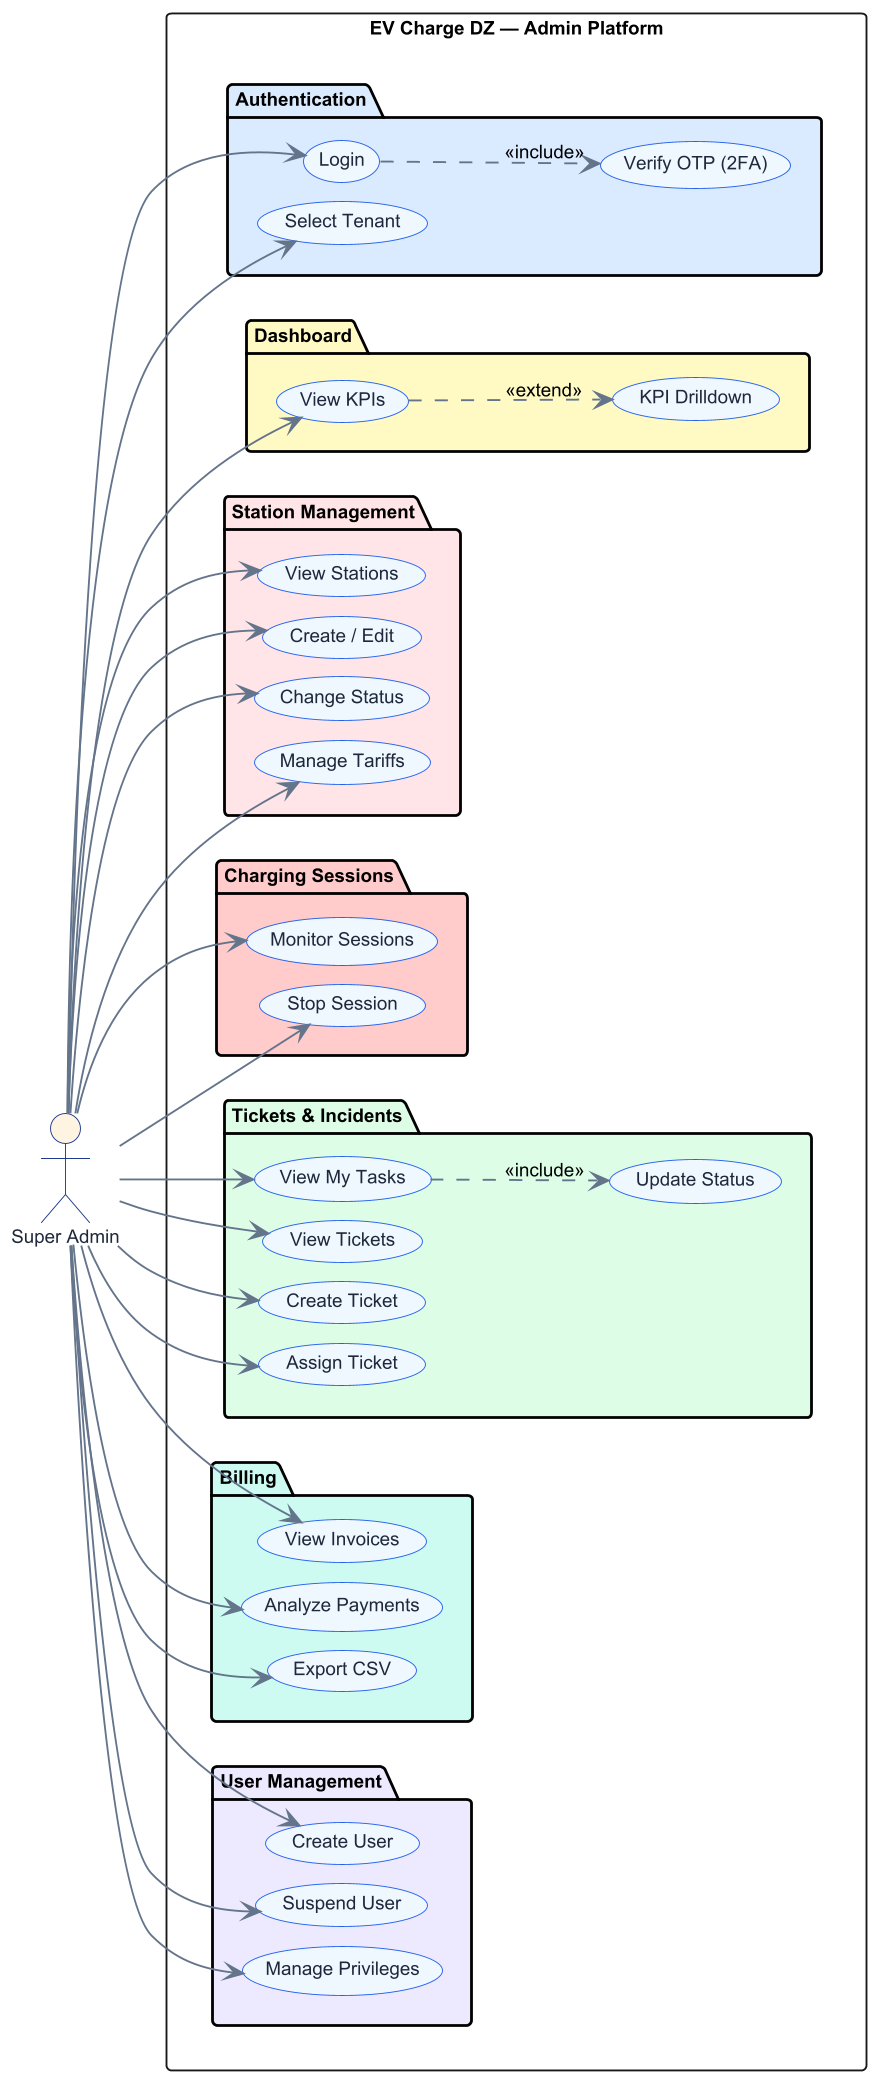
\includegraphics[width=0.72\textwidth, height=0.92\textheight, keepaspectratio]{../diagramme/filz/super_admin.png}
  \caption{Use Case Diagram --- Super Admin}
  \label{fig:usecase-sa}
\end{figure}

\begin{figure}[p]
  \centering
  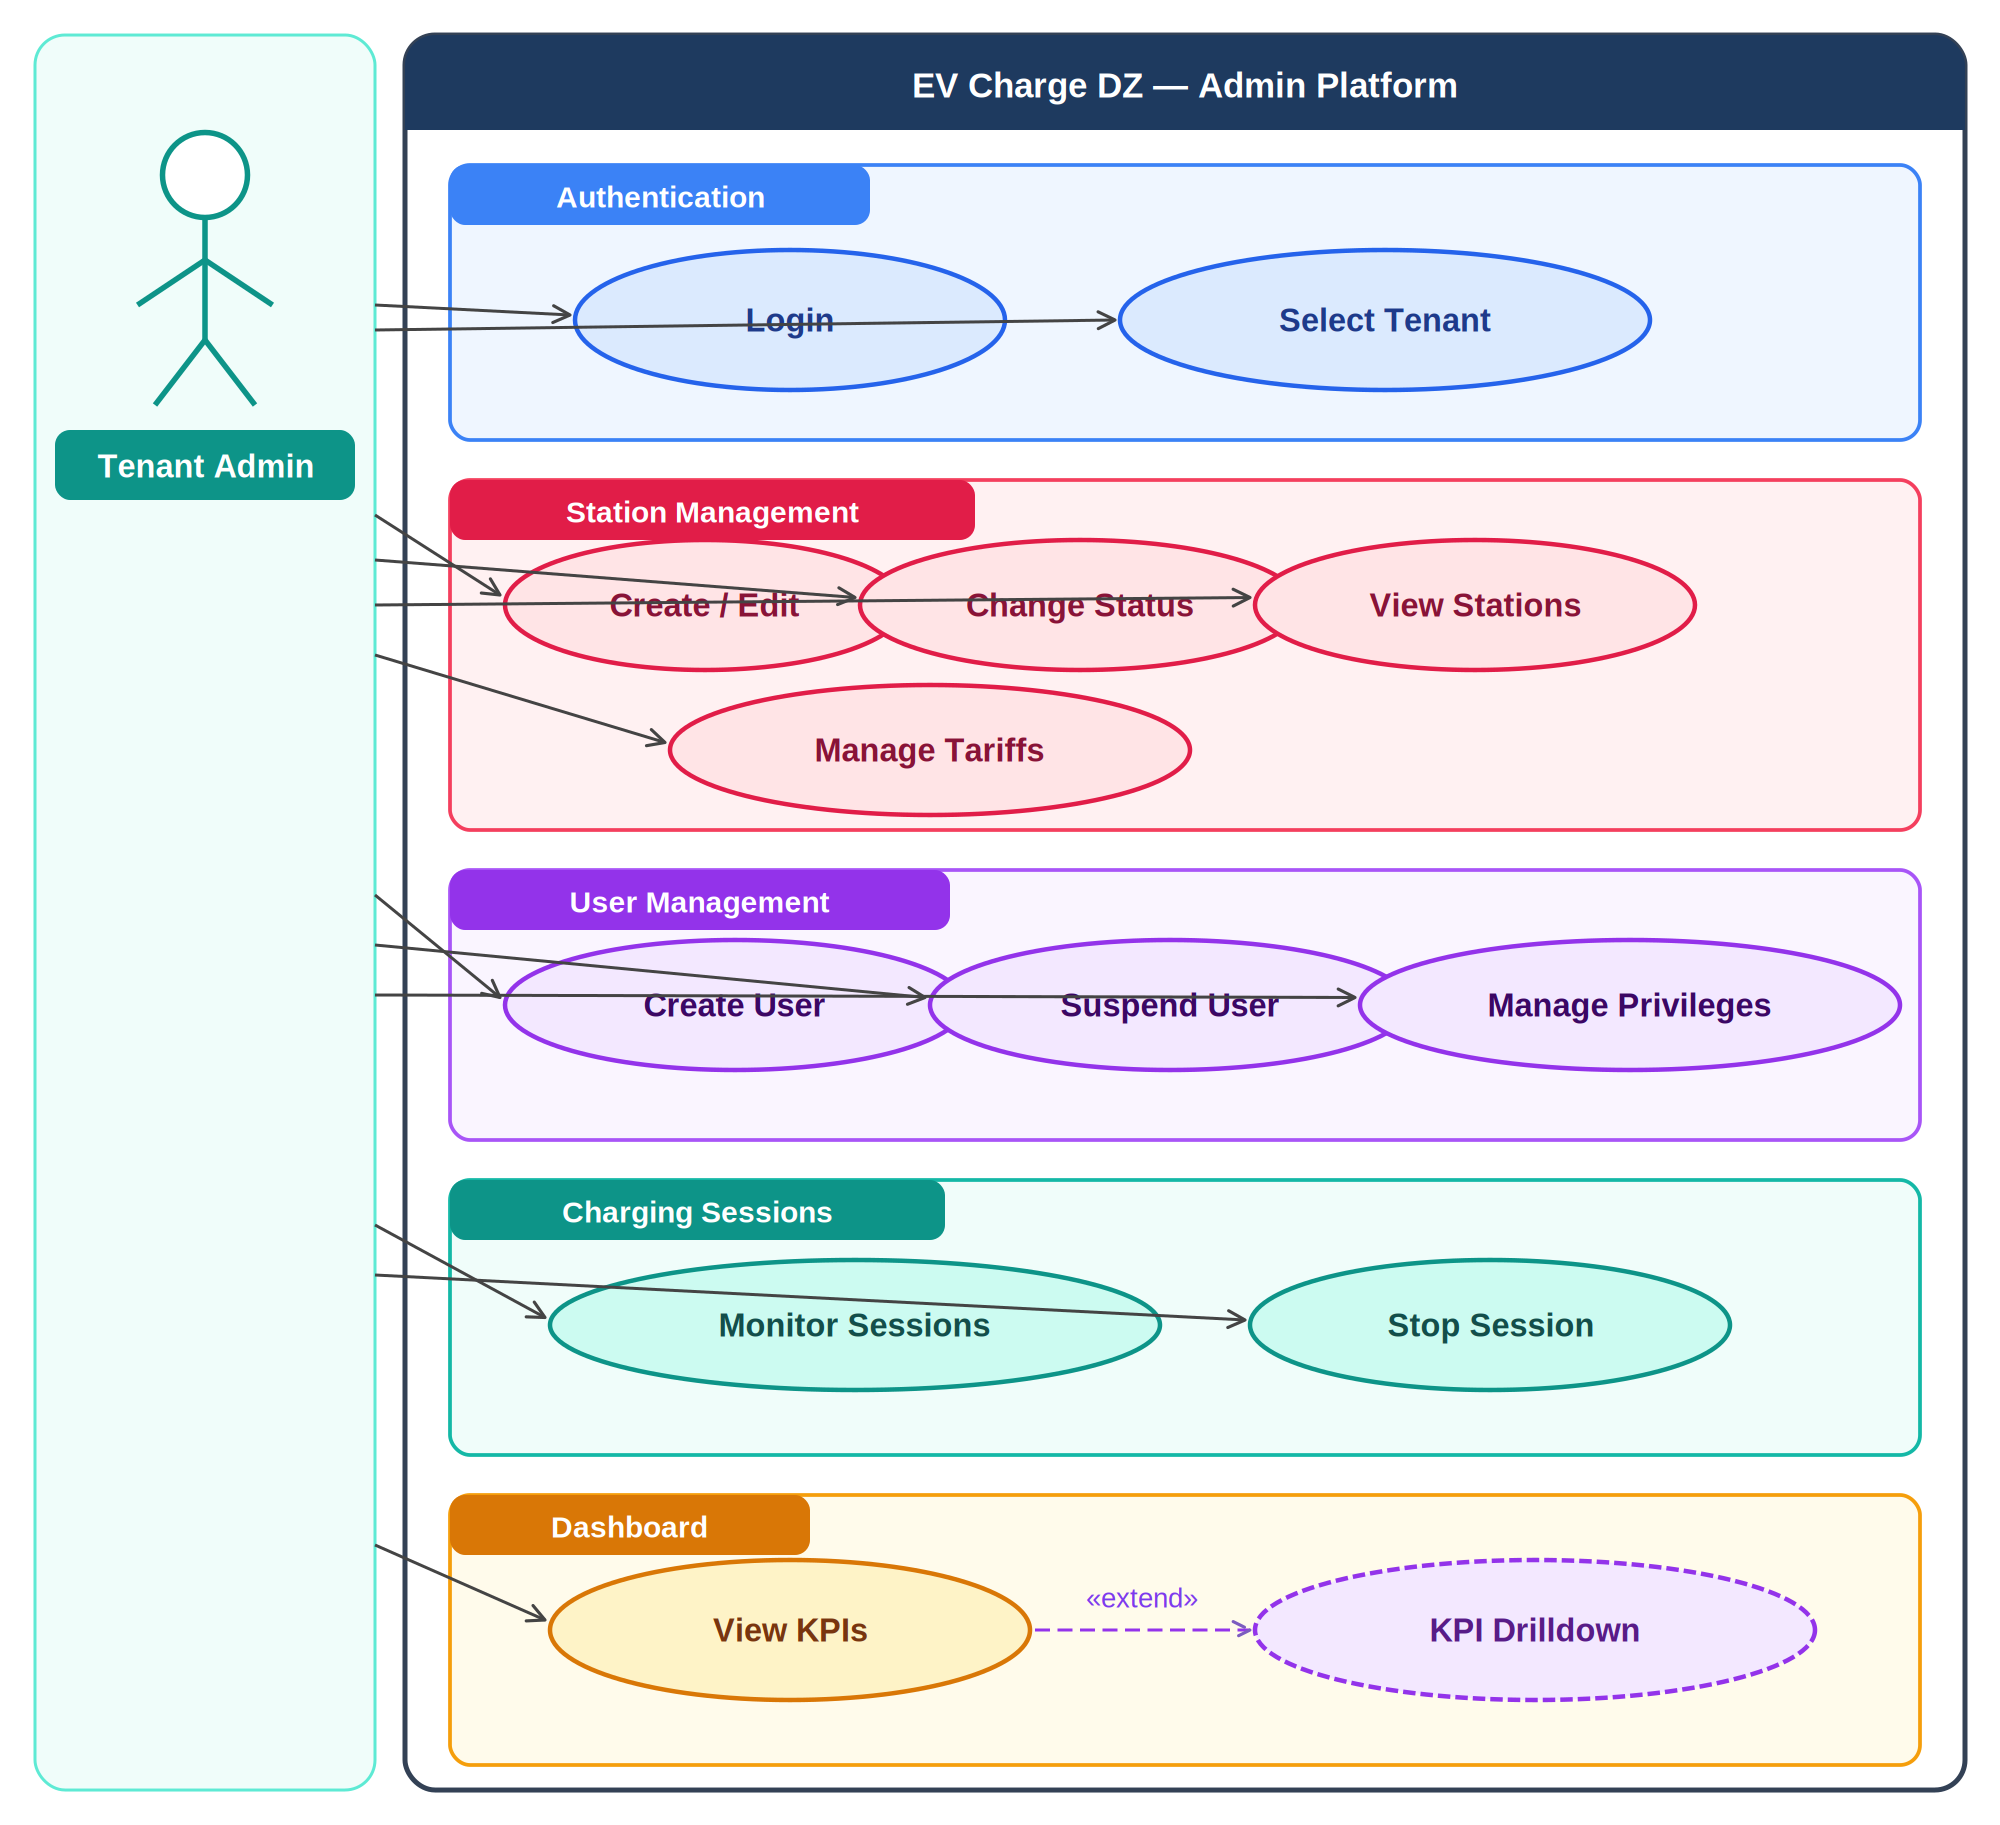
\includegraphics[width=0.72\textwidth, height=0.92\textheight, keepaspectratio]{../diagramme/filz/tenant_admin.png}
  \caption{Use Case Diagram --- Tenant Admin}
  \label{fig:usecase-ta}
\end{figure}

\begin{figure}[p]
  \centering
  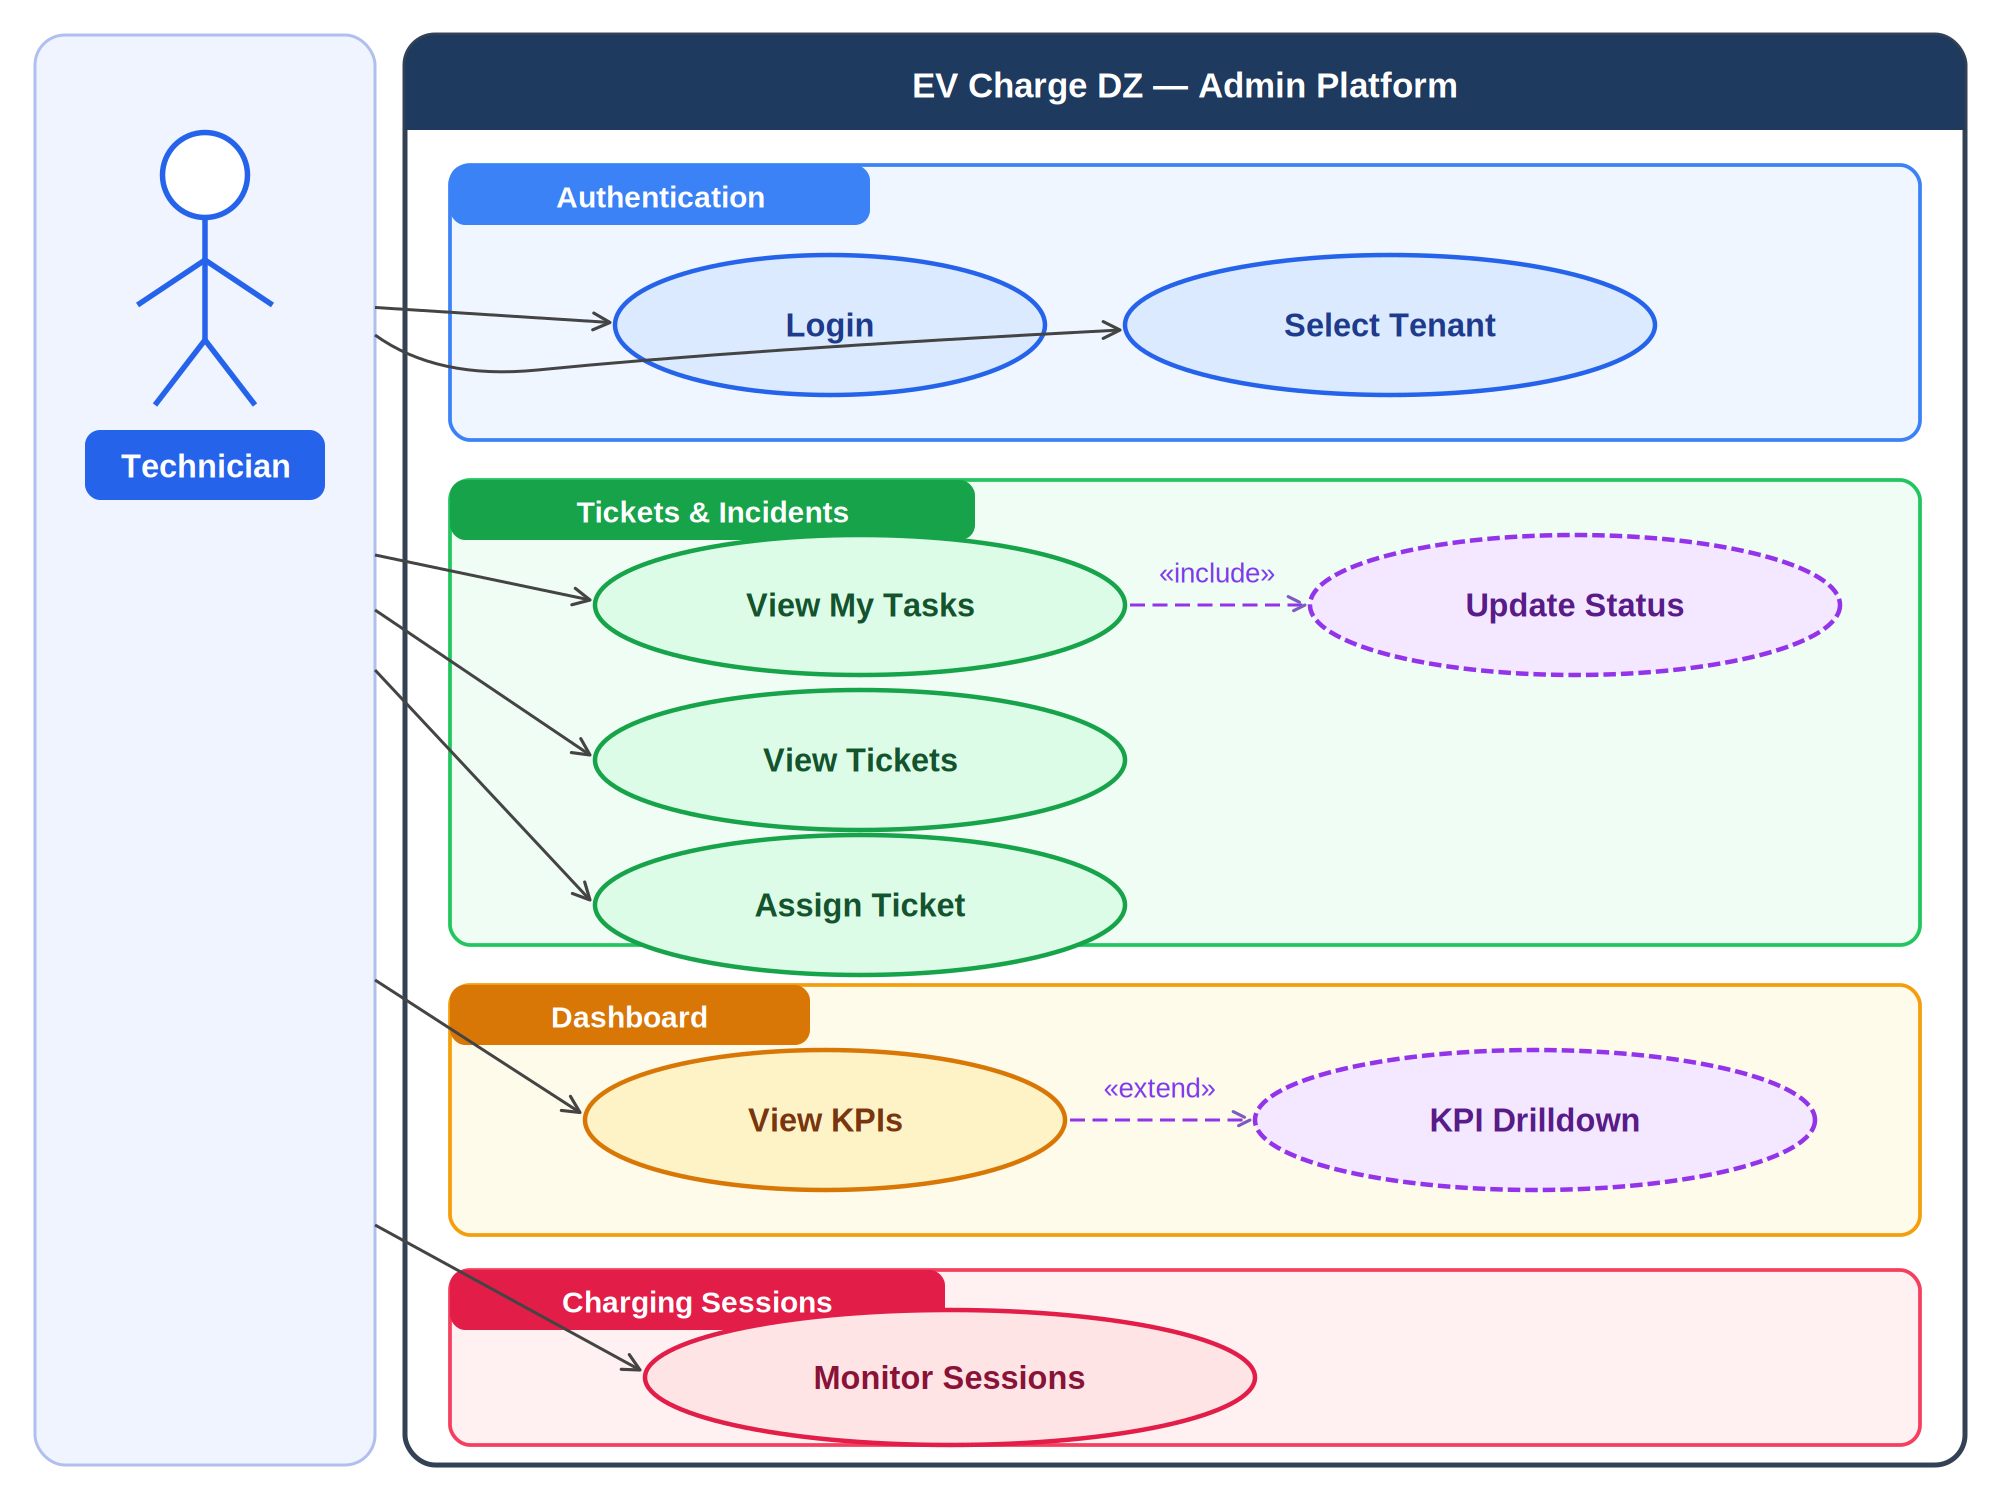
\includegraphics[width=0.72\textwidth, height=0.92\textheight, keepaspectratio]{../diagramme/filz/technician.png}
  \caption{Use Case Diagram --- Technician}
  \label{fig:usecase-tech}
\end{figure}

% ──────────────────────────────────────────────────────────────────────────────
\section{Technical Constraints}

\subsection{Protocol Constraint --- OCPP~1.6}

The platform must implement OCPP~1.6 for station communication~\autocite{ocpp16_ed2}. As
established in Chapter~2, OCPP~2.0.1 was evaluated but excluded due to limited hardware
availability and network infrastructure maturity in Algeria.

\subsection{Regulatory and Market Constraints}

All billing must be expressed in Algerian Dinars~(DZD). Payment integration must support the
CIB interbank card network and local e-payment services, reflecting the payment landscape
available to Algerian EV operators and end users.

\subsection{Network Infrastructure Constraints}

Given variable connectivity conditions in certain Algerian deployment areas, the frontend must
retain functionality in partial offline scenarios. Operators must not lose access to operational
data during temporary backend outages.

% ──────────────────────────────────────────────────────────────────────────────
\section{Conclusion}

This chapter has established the complete requirements baseline for the EV Charge Manager
platform. Ten functional requirements and six non-functional requirements, combined with three
categories of technical and regulatory constraints, define the scope and boundaries of the
system. These requirements directly inform the architectural choices presented in Chapter~4 and
are validated by the implementation demonstrated in Chapter~5.

%%%=============================================================================
%%  CHAPTER 4 — CONCEPTION
%%%=============================================================================

\chapter{EV Charge Manager : Architecture and Design}

This chapter presents the architectural and design decisions for EV Charge Manager, translating
the requirements established in Chapter~3 into a concrete technical blueprint. We describe the
general three-tier architecture, the multi-tenant isolation model, the data model, the user
access control structure, the authentication flow, and the technology stack selected for the
implementation.

% ──────────────────────────────────────────────────────────────────────────────
\section{General Architecture}

The platform follows a standard three-tier architecture:

\begin{itemize}
  \item \textbf{Presentation Tier}: A single-page application (SPA) built with React~18 and
        TypeScript~\autocite{react_docs, typescript_docs}, bundled with Vite~\autocite{vite_docs}. It
        runs entirely in the browser and communicates with the backend over HTTP/JSON.

  \item \textbf{Logic Tier}: A Node.js REST API built with Express.js~\autocite{nodejs_express},
        responsible for authentication, data validation, and business logic.

  \item \textbf{Data Tier}: A MySQL~8 relational database~\autocite{mysql_docs} storing all
        operational data across 13 tables: tenants, users, privileges, user privileges,
        mobile app users, stations, connectors, charging sessions, tickets, ticket activities,
        billing records, alerts, and push notifications.
\end{itemize}

The frontend communicates with the backend via a centralized API client module. All requests are
authenticated using JSON Web Tokens (JWT)~\autocite{rfc7519}. The application is designed to
degrade gracefully: when the backend is unreachable, it falls back to locally persisted data
(browser \texttt{localStorage}) and notifies the operator with a visible offline-mode banner.

% ──────────────────────────────────────────────────────────────────────────────
\section{Technology Stack}

\begin{table}[h!]
  \centering
  \caption{EV Charge Manager : Technology Stack}
  \label{tab:tech-stack}
  \renewcommand{\arraystretch}{1.3}
  \begin{tabular}{|>{\bfseries}p{3.8cm}|p{4cm}|p{5.5cm}|}
    \hline
    Layer              & Technology            & Role \\ \hline
    Language           & TypeScript~5          & Type-safe JavaScript~\autocite{typescript_docs} \\ \hline
    UI Framework       & React~18              & Component-based SPA~\autocite{react_docs} \\ \hline
    Build Tool         & Vite~6                & Fast dev server and bundler~\autocite{vite_docs} \\ \hline
    UI Components      & shadcn/ui + Radix~UI  & Accessible component primitives \\ \hline
    Styling            & Tailwind CSS          & Utility-first CSS~\autocite{tailwindcss_docs} \\ \hline
    Charts             & Recharts              & SVG-based data visualisation~\autocite{recharts_docs} \\ \hline
    Routing            & React Router~v7       & Client-side navigation~\autocite{reactrouter_docs} \\ \hline
    Map                & Leaflet / OpenStreetMap & Interactive station map \\ \hline
    Backend            & Node.js + Express.js  & REST API server~\autocite{nodejs_express} \\ \hline
    Database           & MySQL~8               & Relational data storage~\autocite{mysql_docs} \\ \hline
    Authentication     & JWT + OTP (2FA)       & Stateless token auth~\autocite{rfc7519} \\ \hline
    Charging Protocol  & OCPP~1.6              & Station communication~\autocite{ocpp16_ed2} \\ \hline
  \end{tabular}
\end{table}

% ──────────────────────────────────────────────────────────────────────────────
\section{Multi-Tenant Architecture}

The platform supports multiple independent operators referred to as \textit{tenants} each
with complete data isolation. Two tenants are currently configured:

\begin{itemize}
  \item \textbf{Sonelgaz}: Algeria's national electricity company and primary EV infrastructure
        operator.
  \item \textbf{SAEIG}: A private EV charging network operator.
\end{itemize}

Tenant isolation is enforced at the database level through a \texttt{tenant\_id} foreign key on
all operational entities (users, stations, charging sessions, tickets, billing records, alerts,
and notifications). At the
application level, a \textit{TenantContext} React context propagates the active tenant across
all components, which filter their data accordingly. Each tenant may also define custom branding
(accent color, logo), providing a white-label experience while sharing common platform
infrastructure.

% ──────────────────────────────────────────────────────────────────────────────
\section{Data Model}

The class diagram in Figure~\ref{fig:class-diagram} presents the database-oriented data model
of EV Charge Manager. The schema comprises 13 tables organised across three concerns:
dashboard staff management (\texttt{users}, \texttt{privileges}, \texttt{user\_privileges}),
mobile driver accounts (\texttt{app\_users}), and operational data (\texttt{stations},
\texttt{connectors}, \texttt{charging\_sessions}, \texttt{tickets}, \texttt{ticket\_activities},
\texttt{billing\_records}, \texttt{alerts}, \texttt{notifications}). All operational entities
carry a \texttt{tenant\_id} foreign key, enforcing the multi-tenant isolation described in the
previous section. Stations expose connectors for session initiation; completed sessions are
aggregated into billing records. Tickets reference both a station and an assigned technician,
and maintain a full activity log through \texttt{ticket\_activities}. The \texttt{app\_users}
table stores mobile driver accounts alongside their FCM device token, which the
\texttt{notifications} table uses to record and target push alerts dispatched from the operator
dashboard.

\medskip
\noindent\textit{Note: The complete class diagram including all enumeration types
(\texttt{UserRole}, \texttt{StationStatus}, \texttt{SessionStatus}, etc.) is provided in
Appendix~\ref{app:class-diagram-full} for reference.}

\begin{figure}[p]
  \centering
  \makebox[\textwidth]{
\includegraphics[width=1.25\textwidth, keepaspectratio]{../diagramme/ClassDiag.png}}
  \caption{Class Diagram  EV Charge DZ (Database-Oriented)}
  \label{fig:class-diagram}
\end{figure}

% ──────────────────────────────────────────────────────────────────────────────
\section{User Roles and Access Control}

The platform implements Role-Based Access Control (RBAC) with three distinct user roles:

\begin{table}[h!]
  \centering
  \caption{User Roles and Module Access}
  \label{tab:user-roles}
  \renewcommand{\arraystretch}{1.3}
  \begin{tabular}{|>{\bfseries}p{3.2cm}|p{3cm}|p{7cm}|}
    \hline
    Role           & Scope           & Accessible Modules \\ \hline
    super\_admin   & All tenants     & Dashboard, Stations, Sessions, Billing, Tickets,
                                       Users, Notifications \\ \hline
    tenant\_admin  & Own tenant only & Dashboard, Stations, Sessions, Billing, Tickets,
                                       Notifications \\ \hline
    technician     & Own tasks only  & My Tasks (assigned maintenance tickets) \\ \hline
  \end{tabular}
\end{table}

Beyond role assignment, the platform supports thirteen fine-grained privilege types organised
into four profiles aligned with the actual roles of the system.
Table~\ref{tab:privilege-matrix} details the exact privilege set assigned to each profile.
The \textit{super\_admin} profile grants unrestricted access across all 13 flags, covering every
module of the platform and all tenants.
The \textit{tenant\_admin} profile covers the full operational scope of a tenant — stations,
sessions, billing, and tickets — but excludes user management and global settings, which remain
reserved for the super administrator.
The \textit{finance\_admin} profile is scoped to billing and reporting operations, with
contextual read access to stations, sessions, and tickets; access to user management and station
control is intentionally withheld.
The \textit{technician} profile is the most restricted, limited to the flags strictly required
for on-site infrastructure maintenance, and explicitly omits billing and user data in compliance
with GDPR data-minimisation requirements~\autocite{gdpr2016}.
Routes in the frontend are guarded by a \texttt{RequireAuth} component that verifies both
authentication and role before rendering any protected page.

\begin{table}[h!]
  \centering
  \caption{Privilege Matrix --- Assigned Flags per Role Profile}
  \label{tab:privilege-matrix}
  \renewcommand{\arraystretch}{1.25}
  \setlength{\tabcolsep}{4pt}
  \begin{tabular}{|>{\small\ttfamily}l|
                  >{\centering\arraybackslash}p{1.7cm}|
                  >{\centering\arraybackslash}p{1.8cm}|
                  >{\centering\arraybackslash}p{1.8cm}|
                  >{\centering\arraybackslash}p{1.8cm}|}
    \hline
    \normalfont\textbf{Privilege flag} &
    \textbf{super\_ admin} &
    \textbf{tenant\_ admin} &
    \textbf{technician} &
    \textbf{finance\_ admin} \\ \hline
    users\_view       & \checkmark &            &            & \checkmark \\ \hline
    users\_manage     & \checkmark &            &            &            \\ \hline
    stations\_view    & \checkmark & \checkmark & \checkmark & \checkmark \\ \hline
    stations\_manage  & \checkmark & \checkmark & \checkmark &            \\ \hline
    sessions\_view    & \checkmark & \checkmark & \checkmark & \checkmark \\ \hline
    sessions\_control & \checkmark & \checkmark & \checkmark &            \\ \hline
    tickets\_view     & \checkmark & \checkmark & \checkmark & \checkmark \\ \hline
    tickets\_manage   & \checkmark & \checkmark & \checkmark &            \\ \hline
    billing\_view     & \checkmark & \checkmark &            & \checkmark \\ \hline
    billing\_manage   & \checkmark & \checkmark &            & \checkmark \\ \hline
    reports\_view     & \checkmark & \checkmark &            & \checkmark \\ \hline
    reports\_export   & \checkmark & \checkmark &            & \checkmark \\ \hline
    settings\_manage  & \checkmark &            &            &            \\ \hline
    \normalfont\textbf{Total flags} & \normalfont 13 & \normalfont 10 & \normalfont 6 & \normalfont 8 \\ \hline
  \end{tabular}
\end{table}

Table~\ref{tab:privilege-matrix} reveals a clear privilege hierarchy across the four role
profiles. The \textit{super\_admin} holds all 13 flags, confirming its unrestricted cross-tenant
authority over every module of the platform.
The \textit{tenant\_admin} profile, with 10 flags, covers the full operational scope of a
tenant while remaining isolated from global user management and platform settings.
The \textit{finance\_admin} profile holds 8 flags focused exclusively on billing, reporting,
and contextual read access, without any control over infrastructure or users.
The \textit{technician} profile is the most restricted at 6 flags, retaining only what is
strictly necessary for on-site maintenance; access to billing and user data is intentionally
excluded to comply with the GDPR data-minimisation principle.

% ──────────────────────────────────────────────────────────────────────────────
\section{Authentication Design}

User authentication follows a two-factor flow:

\begin{enumerate}
  \item The user submits their email, password, and tenant identifier on the login screen.
  \item The backend validates the credentials and generates a One-Time Password~(OTP) sent to
        the registered email address.
  \item The user enters the OTP on a dedicated verification screen. On successful validation,
        the backend issues a signed JWT~\autocite{rfc7519}.
  \item All subsequent API requests include the JWT as a \texttt{Bearer} token in the HTTP
        \texttt{Authorization} header. The backend validates the token signature and tenant
        claims on every protected endpoint.
\end{enumerate}

The JWT is stored in the browser's \texttt{localStorage} and is cleared on logout. The
\texttt{RequireAuth} component performs a client-side token presence check and role verification
before rendering any dashboard route. The sequence diagram in Figure~\ref{fig:seq-auth}
illustrates the complete authentication and OTP verification flow for a super administrator.

\begin{figure}[p]
  \centering
  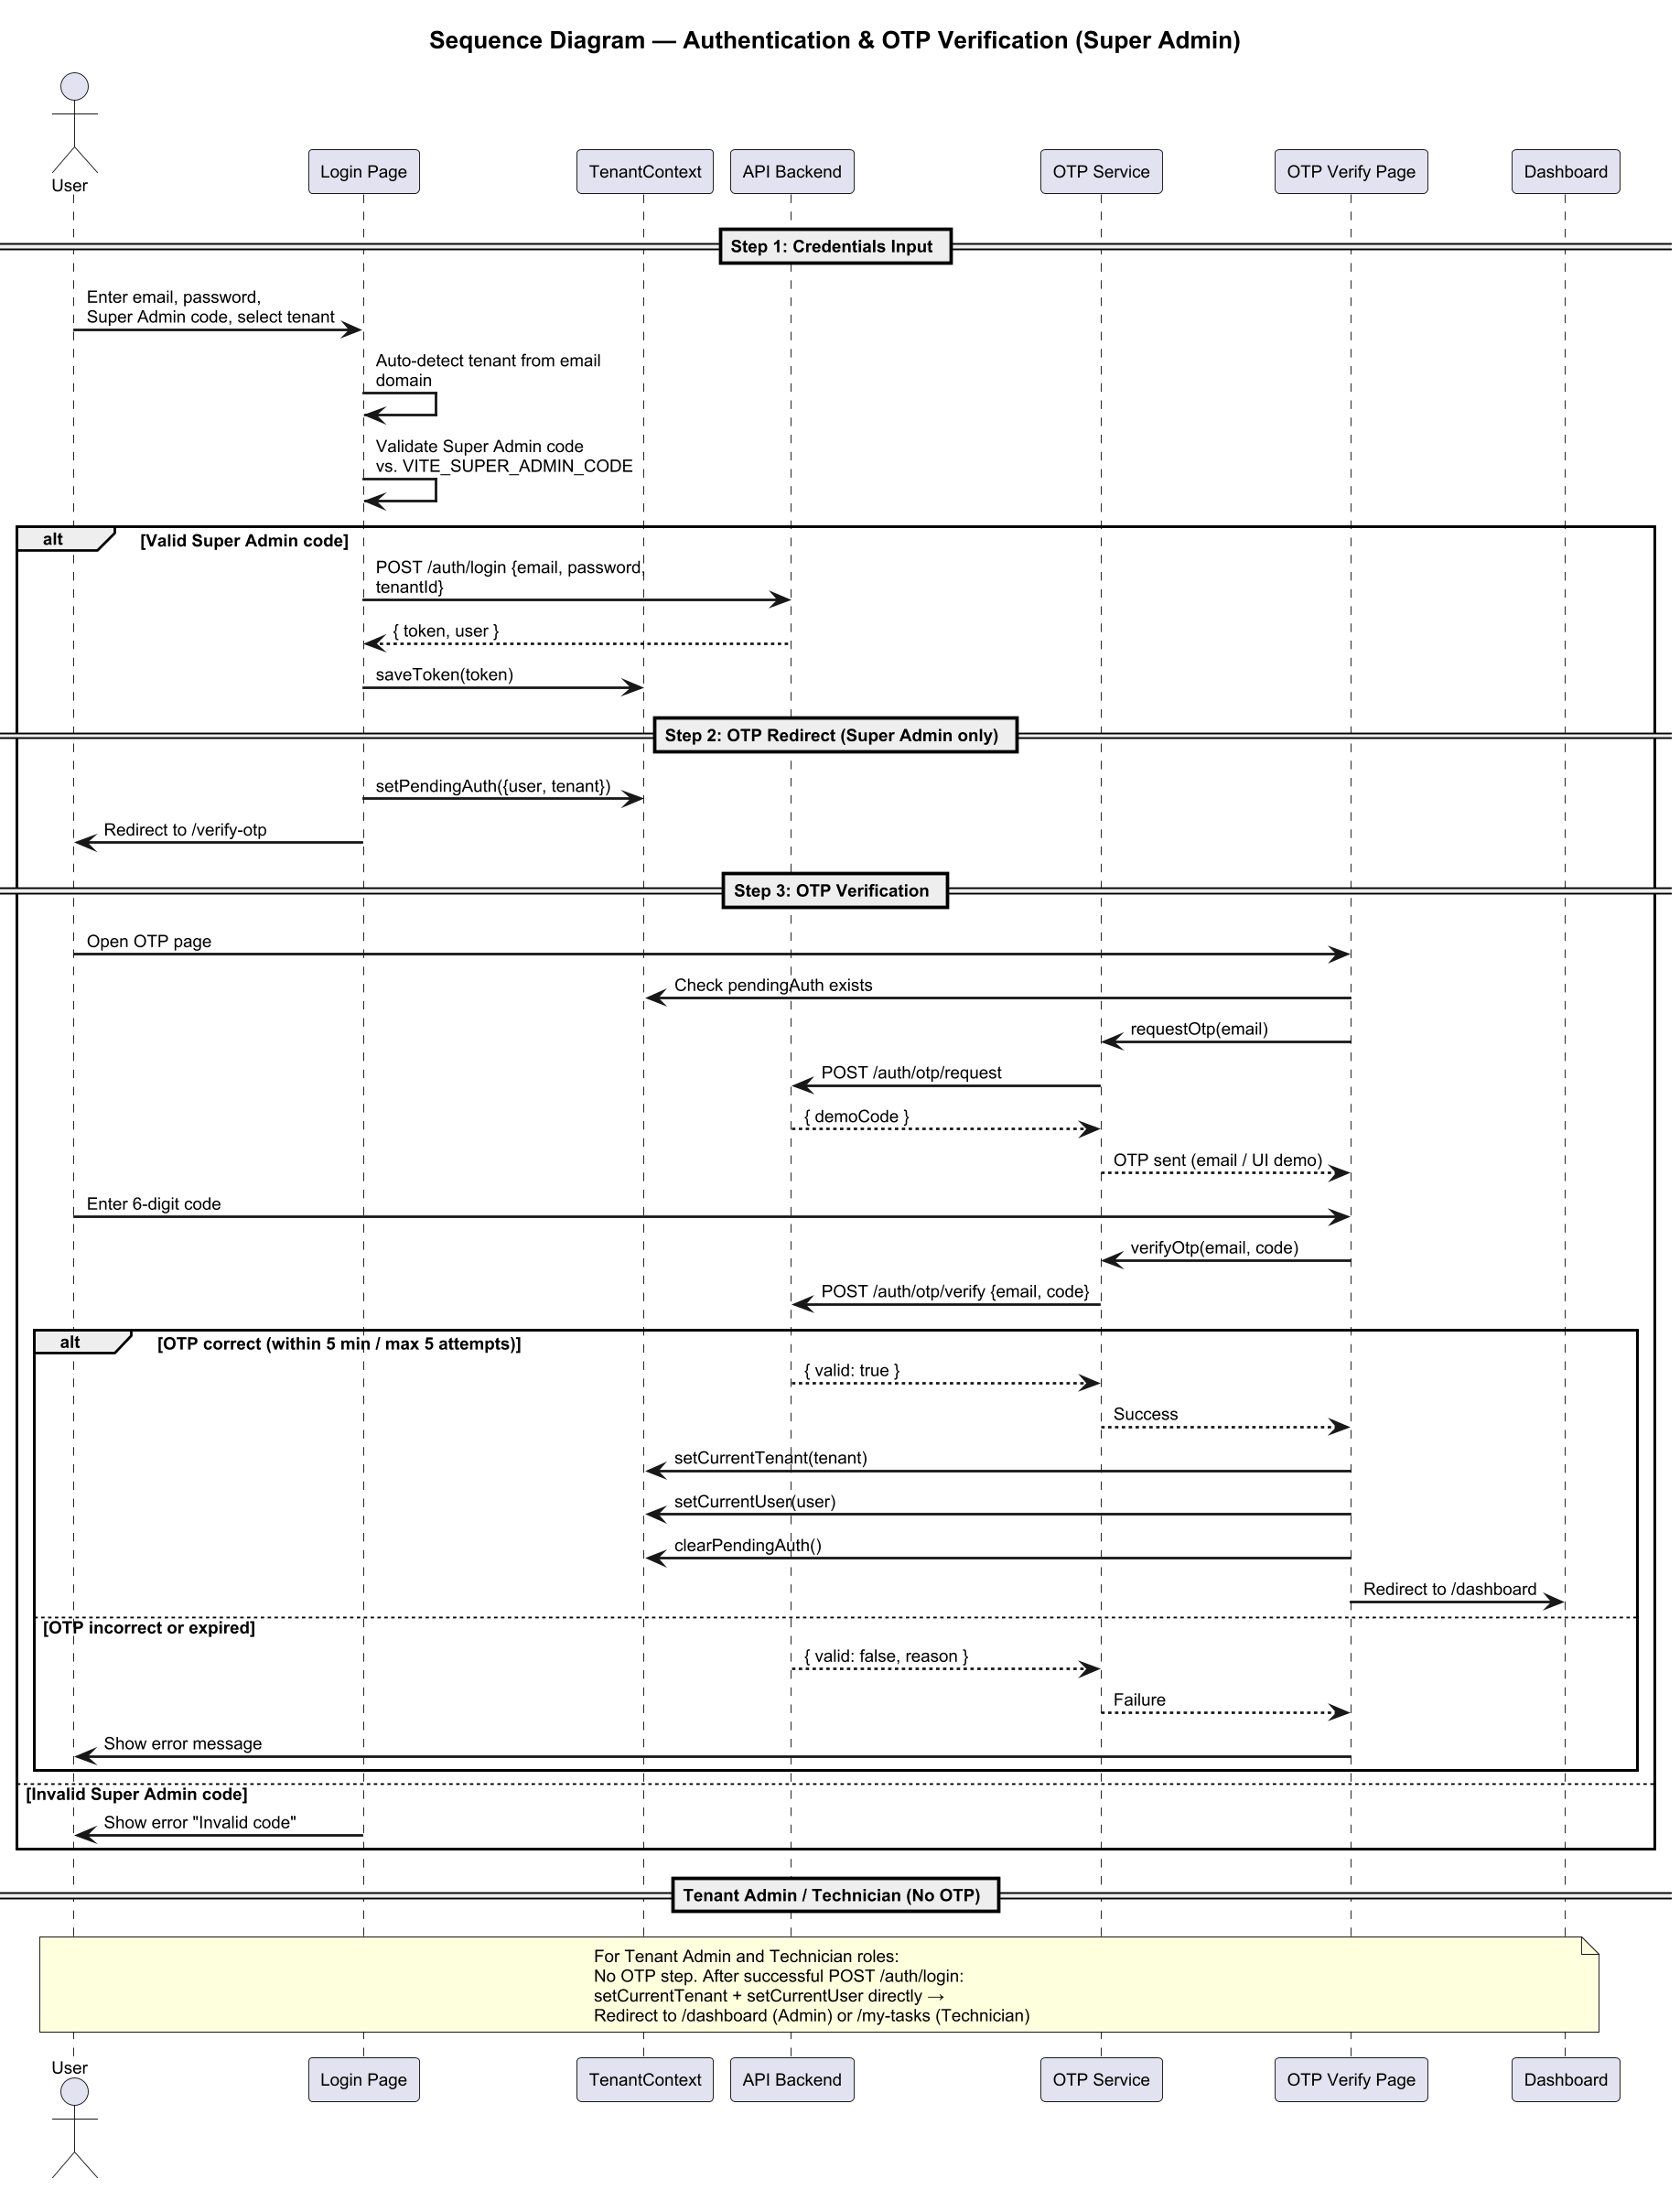
\includegraphics[width=\textwidth, height=0.92\textheight, keepaspectratio]{../diagramme/SeqAuth.png}
  \caption{Sequence Diagram  Authentication and OTP Verification Flow (Super Admin)}
  \label{fig:seq-auth}
\end{figure}

\FloatBarrier
% ──────────────────────────────────────────────────────────────────────────────
\section{Conclusion}

The architectural choices presented in this chapter  three-tier separation, tenant-scoped
database isolation, RBAC with thirteen fine-grained privileges, and two-factor JWT
authentication  directly address the functional and non-functional requirements identified in
Chapter~3. Together they constitute the technical blueprint for the platform implementation
detailed in Chapter~5.

%%%=============================================================================
%%  CHAPTER 5 — RÉALISATION ET TESTS
%%%=============================================================================

\chapter{EV Charge Manager : Implementation and Testing}

This chapter presents the concrete implementation of EV Charge Manager, module by module. Each
section describes the operational interface and behaviour of a functional component, demonstrating
how the design decisions of Chapter~4 translate into a working charging management platform. We
also describe the development environment and conclude with a comprehensive platform summary.

% ──────────────────────────────────────────────────────────────────────────────
\section{Development Environment}

The platform was developed on Windows~11 using Node.js~18~LTS for the backend runtime,
MySQL~8 Community Edition as the database server, and the Vite development server for the
React frontend. Visual Studio Code was used as the primary integrated development environment,
with ESLint and Prettier extensions enforcing code style consistency across the codebase. Git
was used for version control, with the project repository hosted on GitHub.

% ──────────────────────────────────────────────────────────────────────────────
\section{Authentication Interface}

Access to EV~Charge Manager is protected by a tiered authentication scheme adapted to each
role's privilege level. Tenant admins and technicians authenticate with email and password
and are directed immediately to their respective workspace. Super\_admin accounts additionally
require a static platform access code and a time-limited six-digit one-time password (OTP),
forming a three-factor authentication chain that reflects the role's cross-tenant authority.

\begin{figure}[htbp]
  \centering
  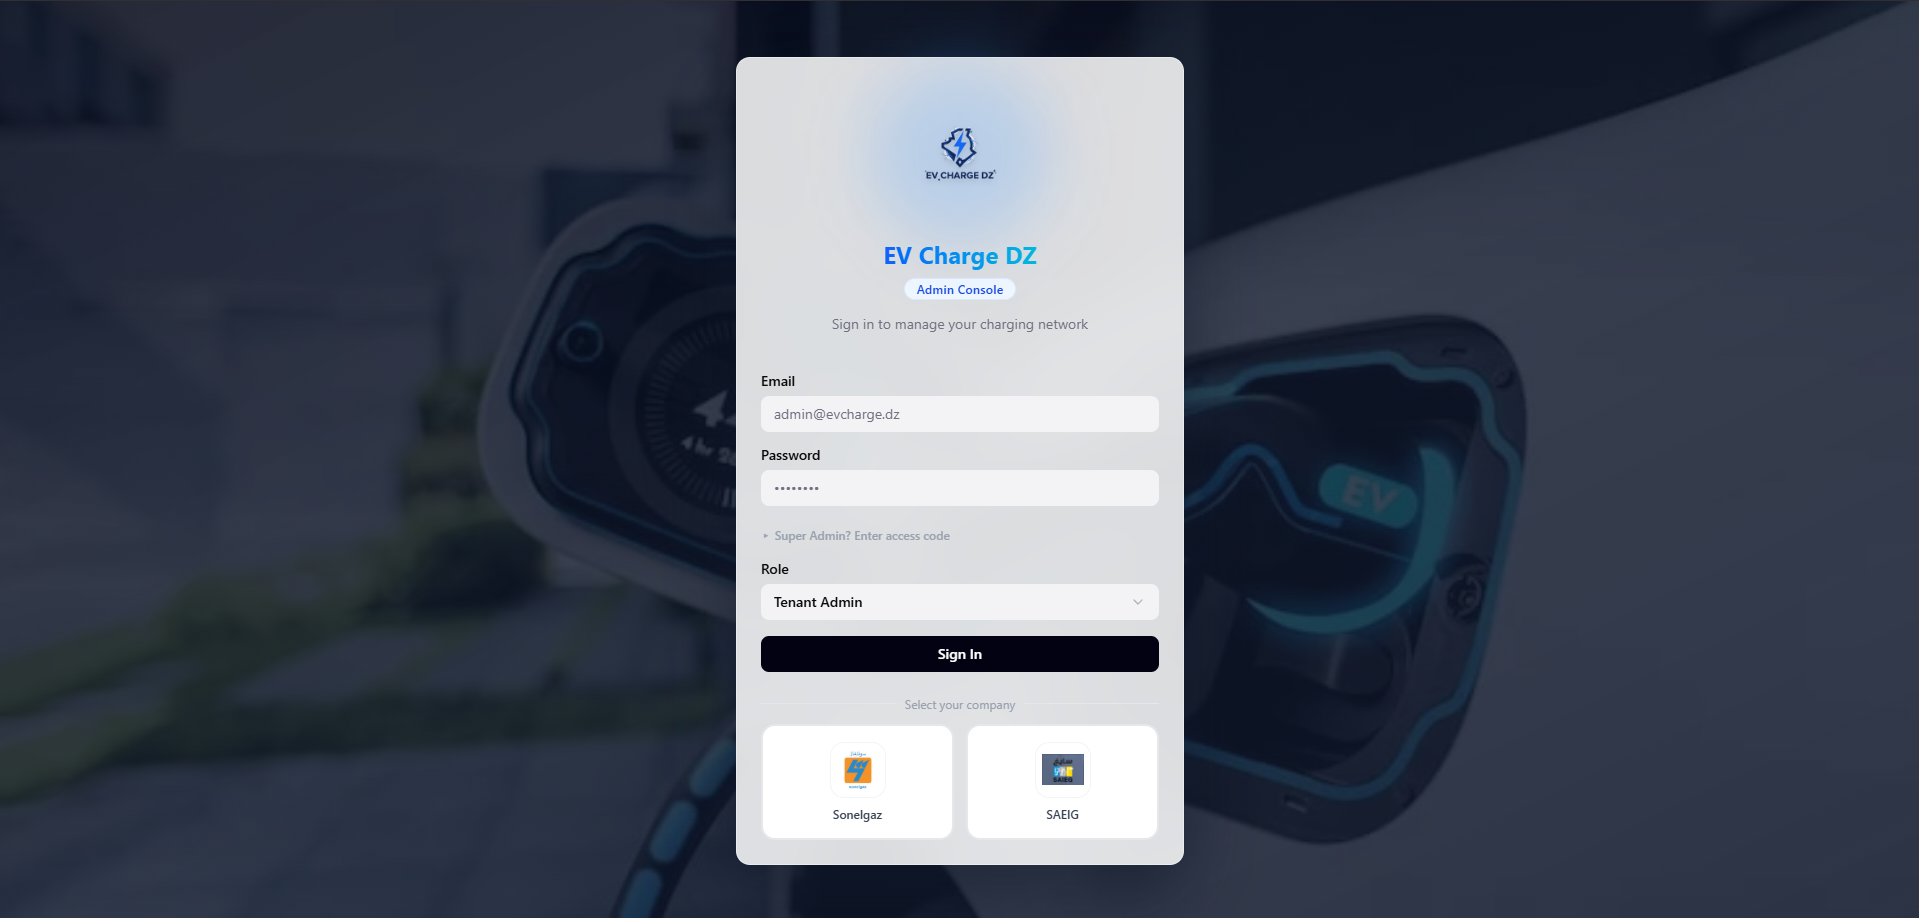
\includegraphics[width=0.65\textwidth]{../../../Screens_4_chapter5/login_page}
  \caption{Login Page --- Credential Entry and Tenant Selection}
  \label{fig:login-page}
\end{figure}

\begin{figure}[htbp]
  \centering
  \begin{minipage}[t]{0.48\textwidth}
    \centering
    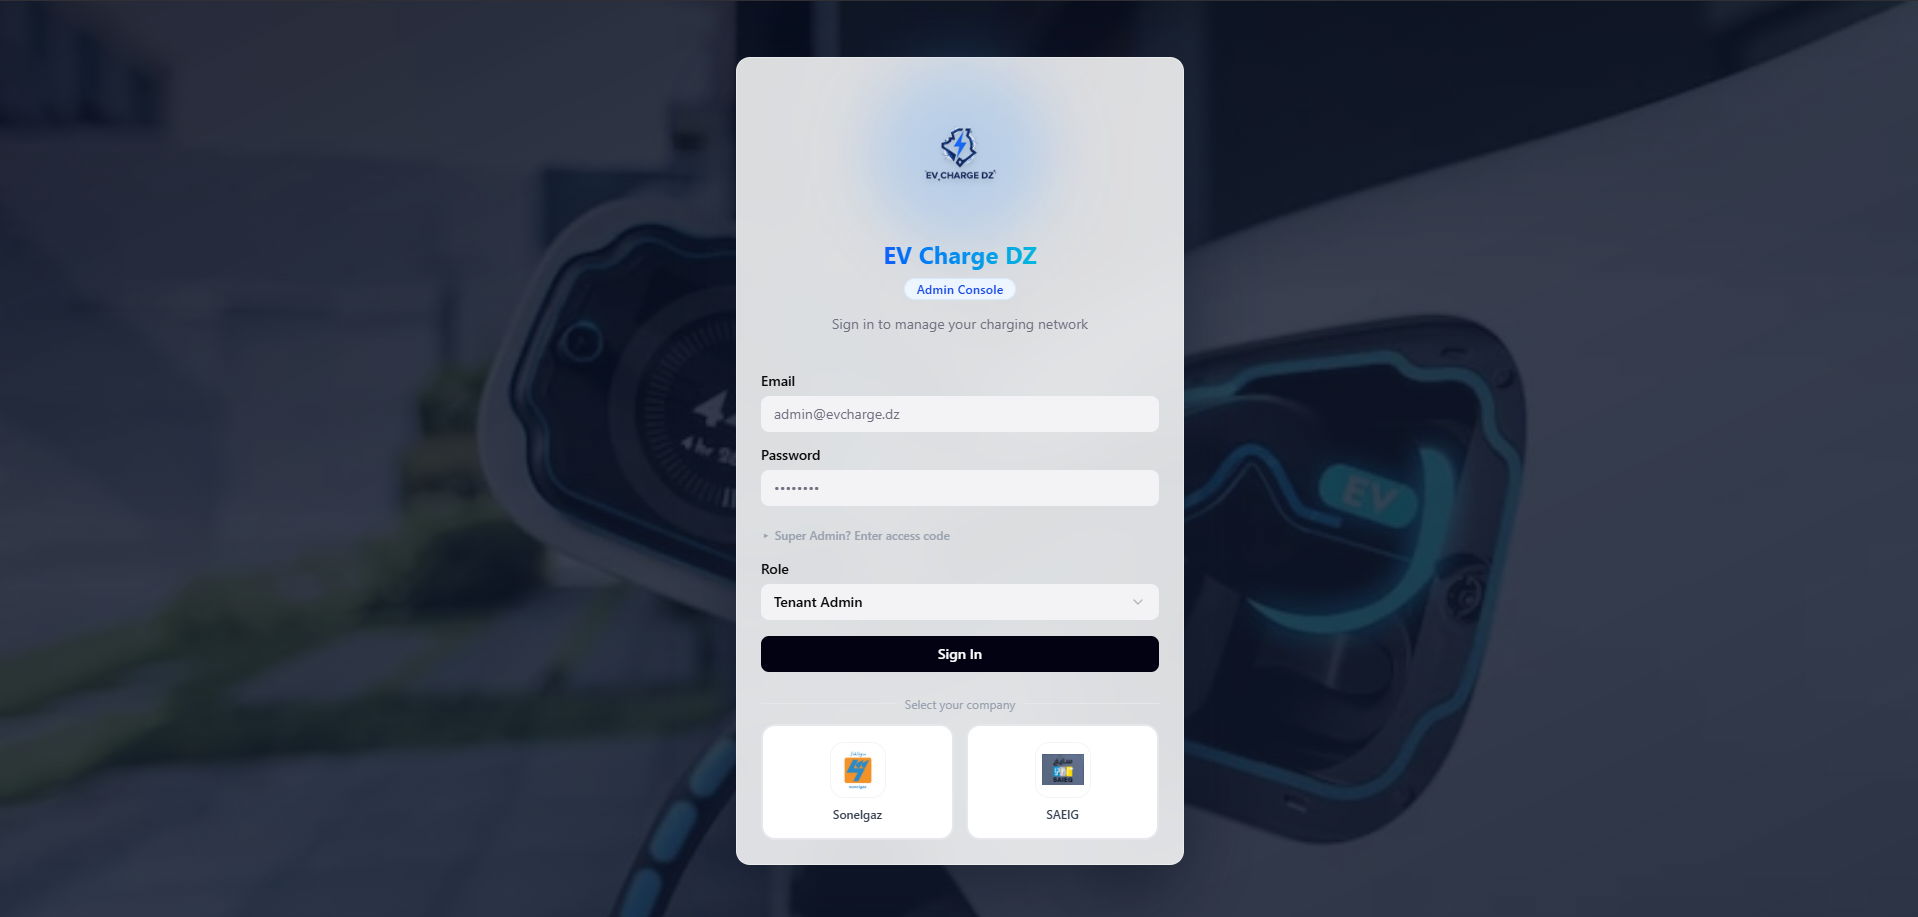
\includegraphics[width=\textwidth]{../../../Screens_4_chapter5/OTP}
    \caption{Login --- Super Admin Access Code Field}
    \label{fig:super-admin-code}
  \end{minipage}
  \hfill
  \begin{minipage}[t]{0.48\textwidth}
    \centering
    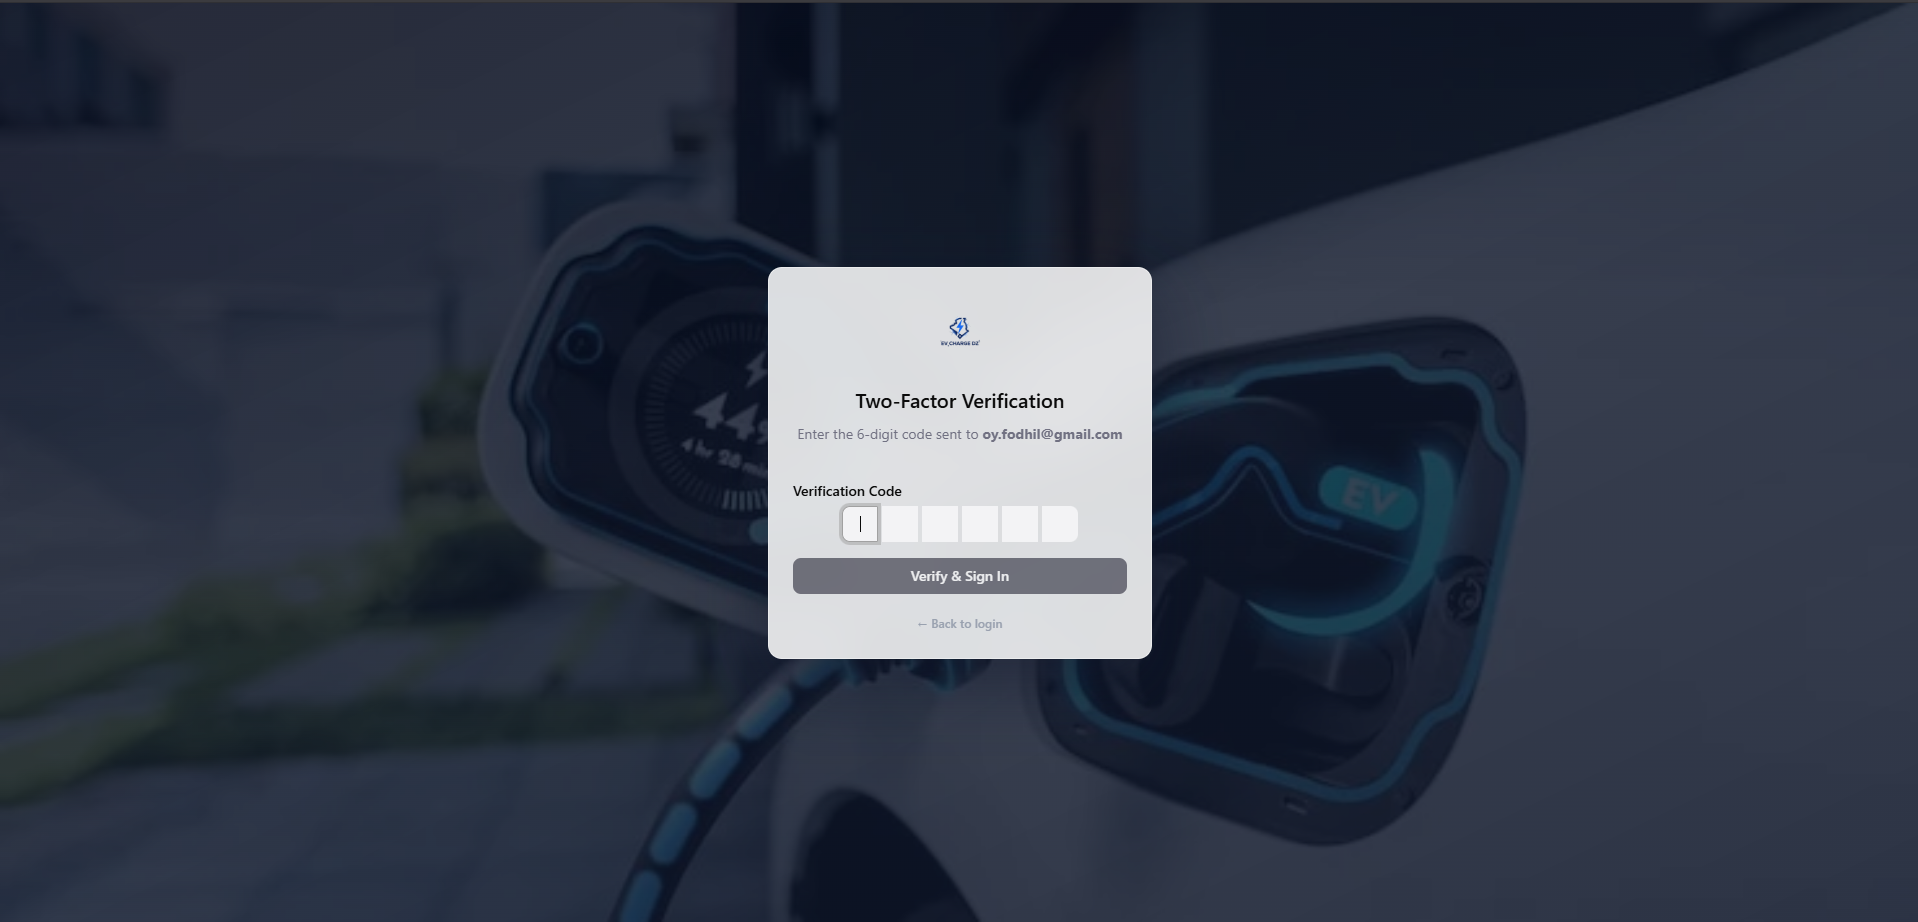
\includegraphics[width=\textwidth]{../../../Screens_4_chapter5/OTP2}
    \caption{Two-Factor Verification --- OTP Entry Step}
    \label{fig:otp-step}
  \end{minipage}
\end{figure}

% ──────────────────────────────────────────────────────────────────────────────
\section{Dashboard Module}

The dashboard provides a real-time overview of the entire charging network through seven Key
Performance Indicators (KPIs), displayed as interactive cards:

\begin{itemize}
  \item \textbf{Active Stations}: Stations in \textit{available} or \textit{charging} status.
  \item \textbf{Offline Stations}: Stations in \textit{fault} or \textit{offline} status.
  \item \textbf{Under Maintenance}: Stations in \textit{maintenance} mode.
  \item \textbf{Active Sessions}: Currently ongoing charging sessions.
  \item \textbf{Energy Delivered}: Total energy dispatched (kWh) over the selected period.
  \item \textbf{Revenue}: Cumulative billing amount (DZD) over the selected period.
  \item \textbf{Network Uptime}: Weighted average station availability rate (\%).
\end{itemize}

Each KPI card displays a trend indicator comparing the current period to the previous one, and
supports a clickable drilldown that opens a contextual side panel. The dashboard also includes:

\begin{itemize}
  \item A 30-day revenue and energy trend chart (multi-line chart built with
        Recharts~\autocite{recharts_docs}).
  \item A connector-type distribution chart (donut chart showing CCS2\,/\,CHAdeMO\,/\,Type~2
        share).
  \item A 24-hour energy consumption curve (hourly resolution).
  \item A real-time alerts feed categorized by severity (info, warning, error).
\end{itemize}

A date filter (Today\,/\,7~Days\,/\,30~Days) is persisted in \texttt{localStorage} to maintain
operator preferences across sessions.

\begin{figure}[htbp]
  \centering
  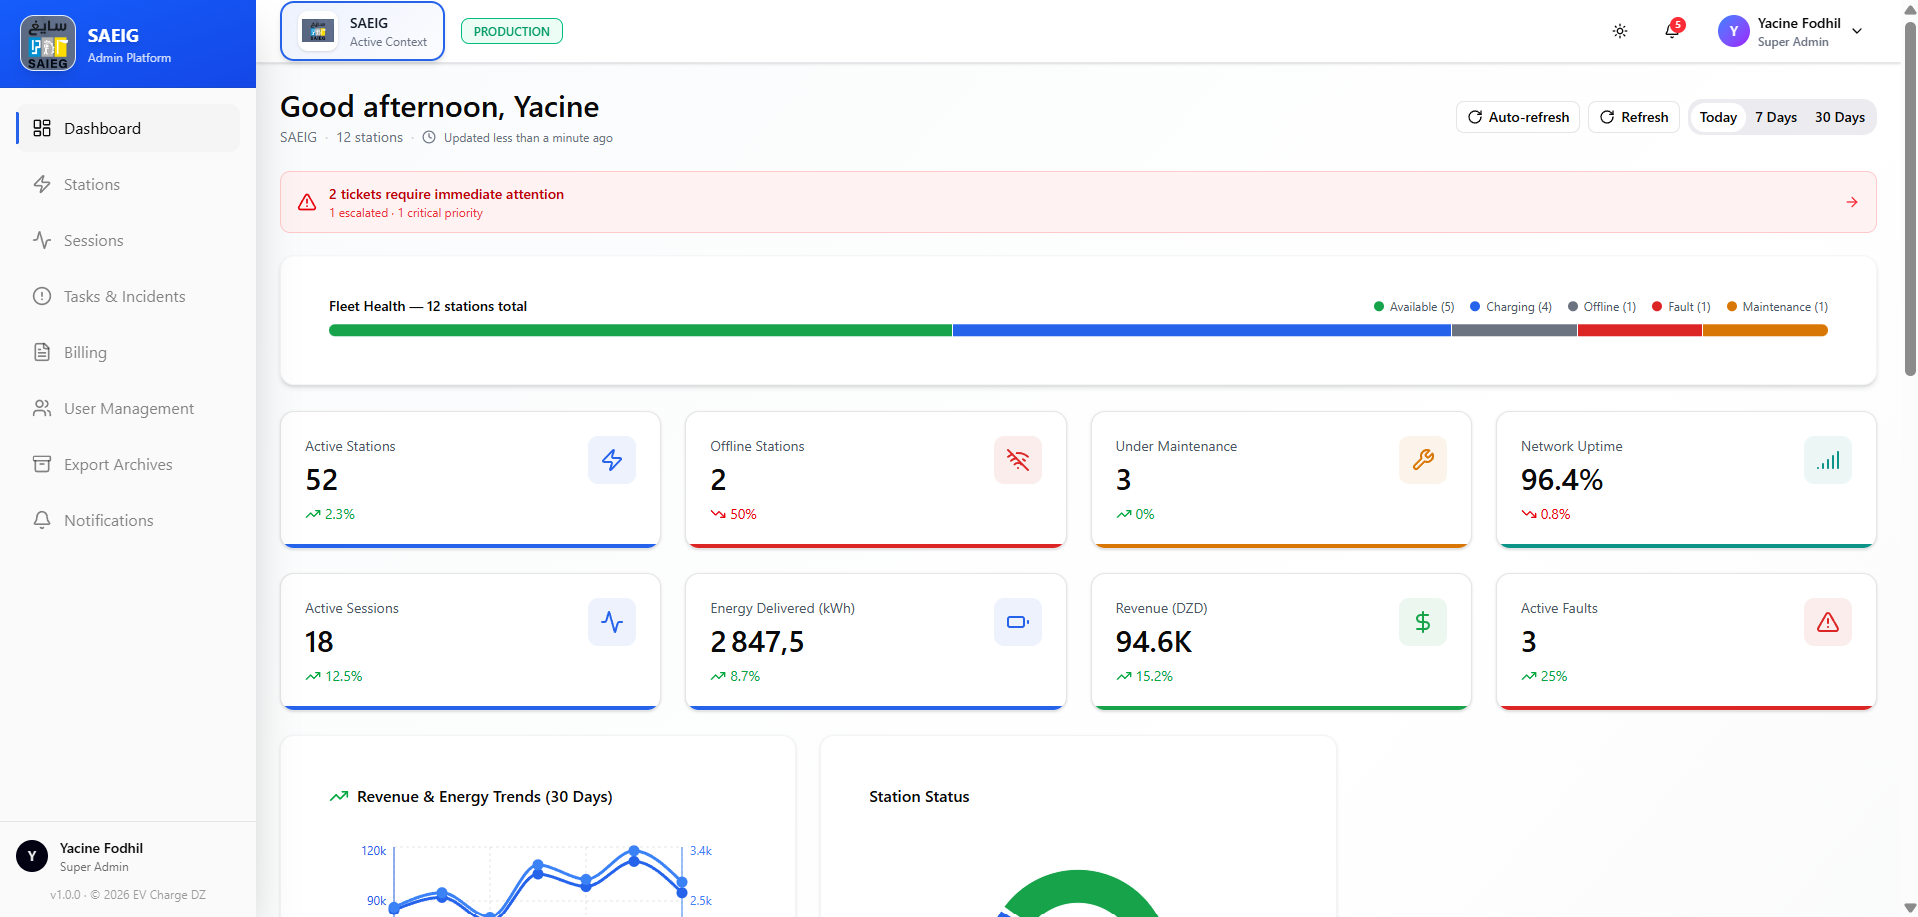
\includegraphics[width=0.95\textwidth]{../../../Screens_4_chapter5/dashboard}
  \caption{Dashboard Module  Real-Time KPI Overview and Trend Charts}
  \label{fig:dashboard}
\end{figure}

% ──────────────────────────────────────────────────────────────────────────────
\section{Station Management Module}

The Stations module provides complete lifecycle management for charging infrastructure. It offers
two complementary views:

\begin{itemize}
  \item \textbf{Table View}: A searchable, filterable table with filters for status and city.
  \item \textbf{Map View}: An interactive Leaflet/OpenStreetMap map showing each station as a
        color-coded marker (by operational status). Clicking a marker reveals station details.
\end{itemize}

\subsection{Connector Standards}

Each station may host multiple connector types simultaneously. The platform supports the three
main standards deployed in Algeria and internationally:

\begin{table}[h!]
  \centering
  \caption{Supported EV Connector Standards}
  \label{tab:connectors}
  \renewcommand{\arraystretch}{1.3}
  \begin{tabular}{|>{\bfseries}p{2.5cm}|p{2cm}|p{3cm}|p{5cm}|}
    \hline
    Type      & Current & Typical Power  & Use Case \\ \hline
    CCS2      & DC      & Up to 350\,kW  & Fast and ultra-fast DC charging \\ \hline
    CHAdeMO   & DC      & Up to 400\,kW  & Japanese DC standard \\ \hline
    Type~2    & AC      & 3.7--22\,kW    & AC home and public slow charging \\ \hline
  \end{tabular}
\end{table}

\subsection{Station Status Values}

Stations cycle through five operational states: \textit{available} (idle, ready),
\textit{charging} (session active), \textit{offline} (network lost), \textit{fault} (hardware
or software fault detected via OCPP~\autocite{ocpp16_ed2}), and \textit{maintenance} (under
scheduled service).

\subsection{Station Actions}

Operators can: enable a station, disable it, toggle maintenance mode, update the tariff
(DZD/kWh), and create a new station with GPS coordinates selected via an embedded location
picker map. All status-changing actions require confirmation through a modal dialog and are
logged in the system audit trail. A CSV export function allows operators to download the
current filtered station list for external reporting.

\begin{figure}[htbp]
  \centering
  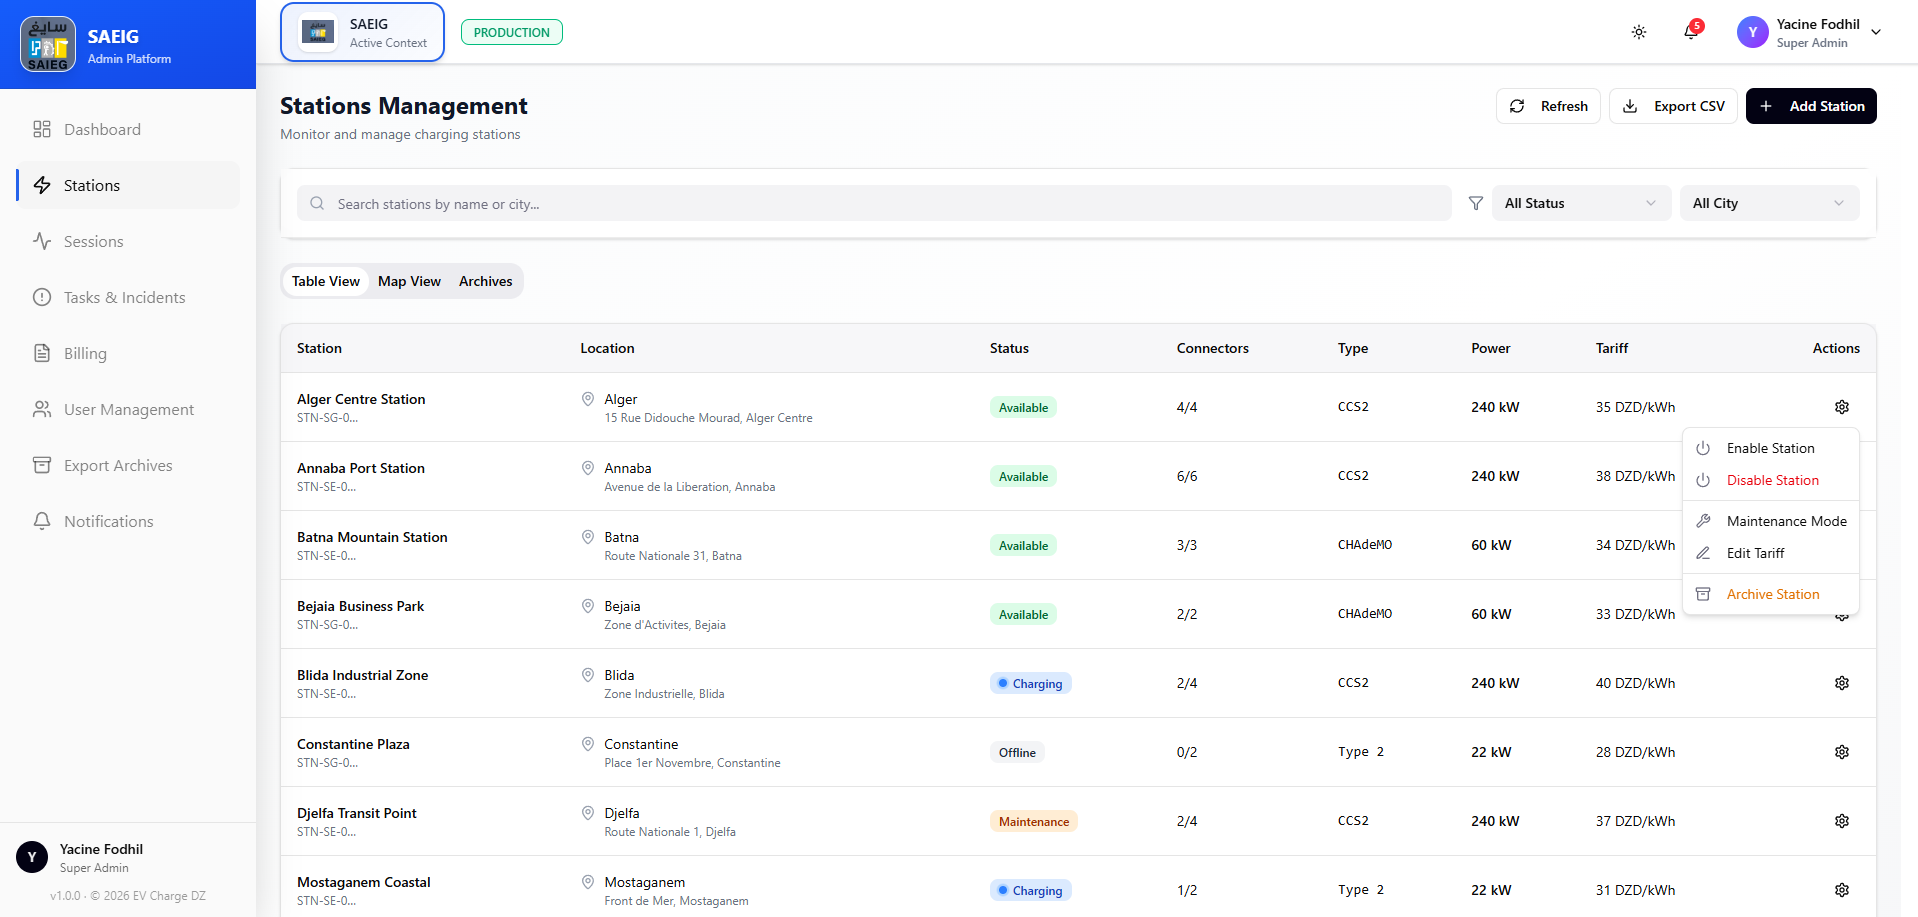
\includegraphics[width=0.95\textwidth]{../../../Screens_4_chapter5/table_view}
  \caption{Station Management --- Table View with Status and City Filters}
  \label{fig:station-table}
\end{figure}

\begin{figure}[htbp]
  \centering
  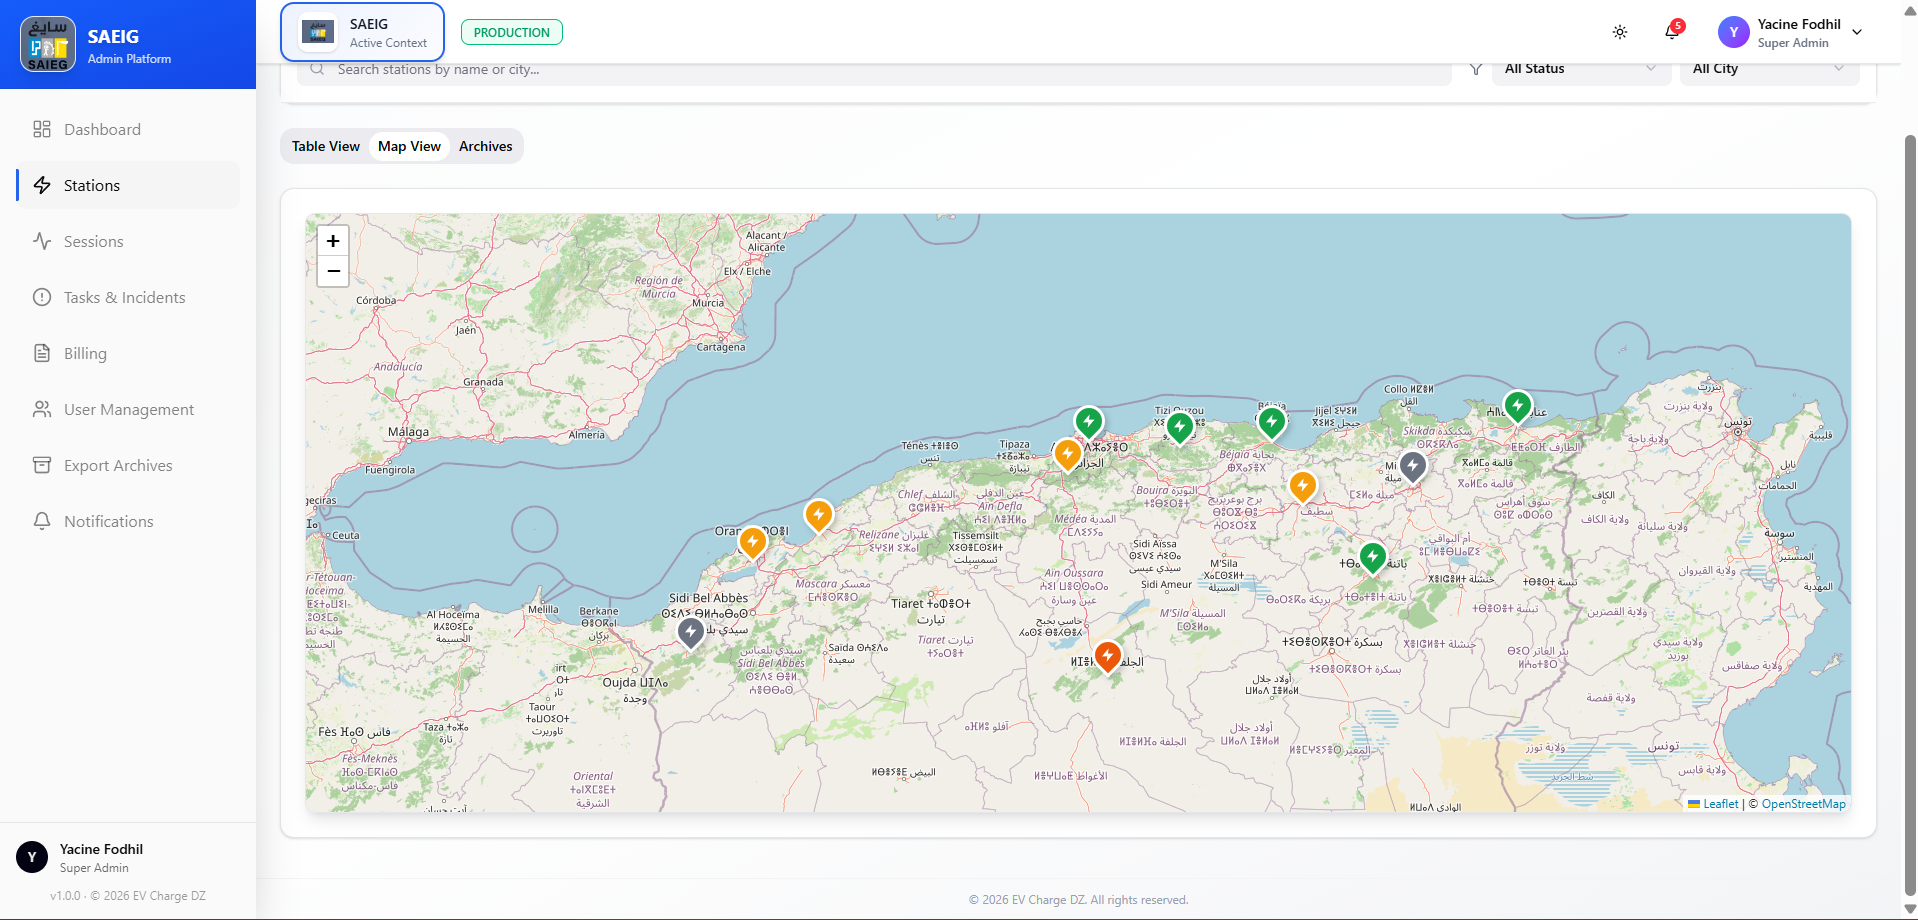
\includegraphics[width=0.95\textwidth]{../../../Screens_4_chapter5/map_view}
  \caption{Station Management  Interactive Map View (Leaflet\,/\,OpenStreetMap)}
  \label{fig:station-map}
\end{figure}

% ──────────────────────────────────────────────────────────────────────────────
\section{Session Monitoring Module}

The Sessions module provides a chronological log of all charging sessions associated with the
active tenant. Each session record contains: a unique session identifier, the source station
name, the connector used, the user's identifier (RFID tag or account ID), session start time,
duration (minutes), energy delivered (kWh), billing amount (DZD), and final status.

Session status values are: \textit{active} (ongoing), \textit{completed} (ended normally),
\textit{stopped} (manually interrupted by user or operator), or \textit{error} (abnormal
termination). Operators can filter sessions by status and station, and export results to CSV.

\begin{figure}[htbp]
  \centering
  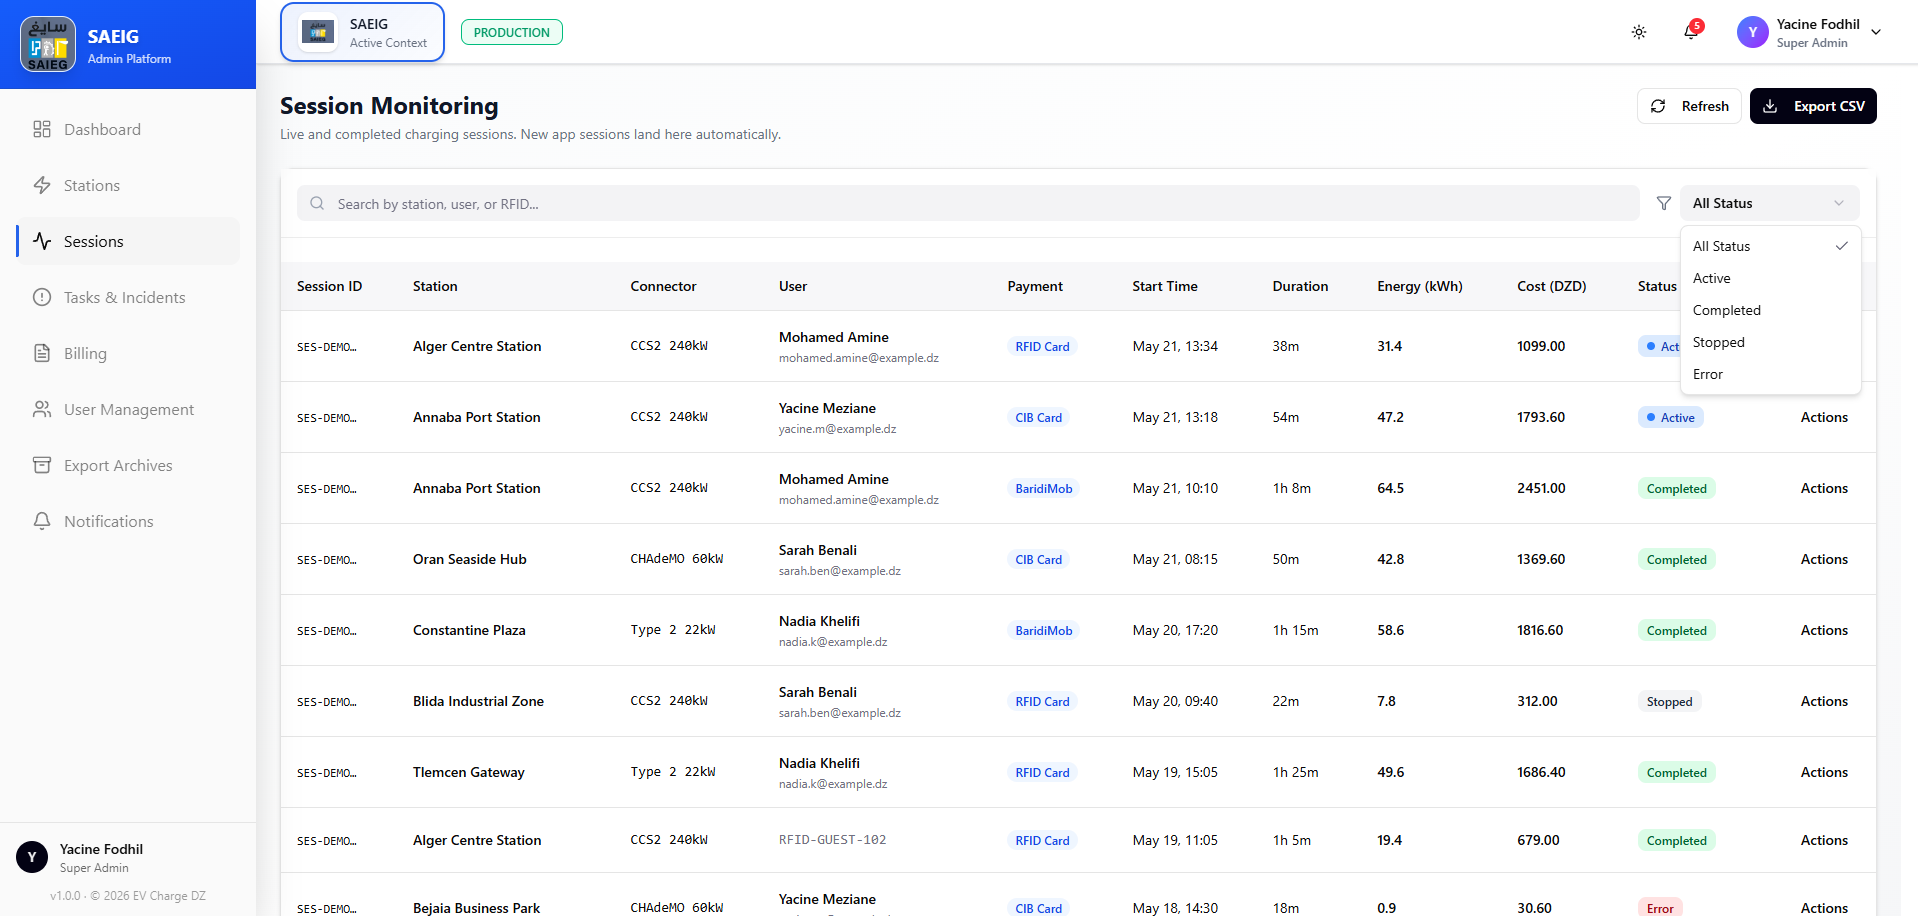
\includegraphics[width=0.95\textwidth]{../../../Screens_4_chapter5/sessions}
  \caption{Session Monitoring Module  Chronological Charging Session Log}
  \label{fig:sessions}
\end{figure}

% ──────────────────────────────────────────────────────────────────────────────
\section{Billing Module}

The Billing module tracks all financial transactions generated by charging sessions. It supports
three payment methods common in the Algerian market:

\begin{itemize}
  \item \textbf{RFID Card}: The most widely deployed method; the customer authenticates using
        an RFID tag registered to their account.
  \item \textbf{CIB (Carte Interbancaire)}: Electronic payment via the Algerian interbank bank
        card network.
  \item \textbf{E-Payment}: Mobile wallet or online payment gateway.
\end{itemize}

Each billing record includes an invoice number, associated station, number of sessions
aggregated, total energy consumed (kWh), total amount (DZD), payment status (paid, unpaid, or
refund), and the payment processing timestamp. The module provides per-method performance
statistics, including transaction count, success rate, failed transaction count, average
processing time (seconds), and revenue contribution percentage.

\begin{figure}[htbp]
  \centering
  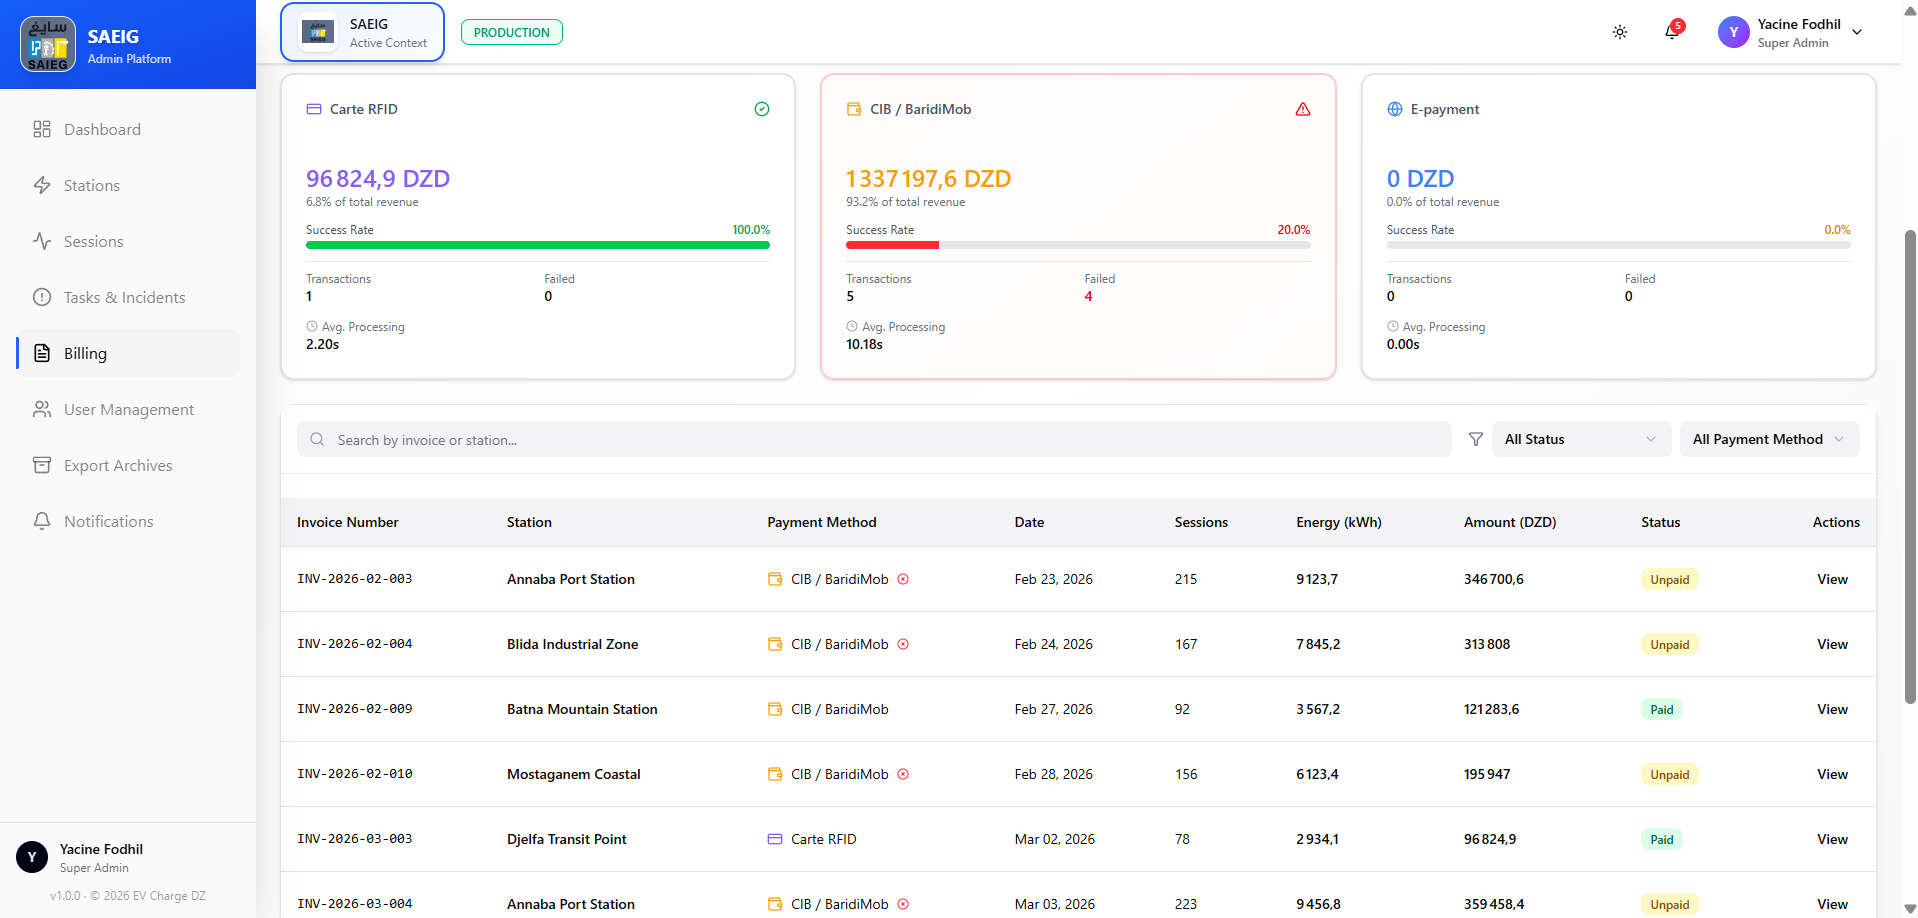
\includegraphics[width=0.95\textwidth]{../../../Screens_4_chapter5/billing}
  \caption{Billing Module  Payment Method Statistics and Invoice Records}
  \label{fig:billing}
\end{figure}

% ──────────────────────────────────────────────────────────────────────────────
\section{Maintenance Ticket System}

The Ticket module implements a structured fault-reporting and maintenance-scheduling workflow.
When a station issue is detected automatically via the alert system or manually by an
operator a ticket is created with the following attributes:

\begin{itemize}
  \item \textbf{Category}: One of six types power failure, screen issue, charger fault,
        system failure, network issue, or scheduled maintenance.
  \item \textbf{Priority}: Low, medium, high, or critical.
  \item \textbf{SLA Deadline}: A contractual resolution deadline tracked and displayed as a
        countdown; breached deadlines trigger automatic escalation.
  \item \textbf{Assignment}: The ticket is assigned to a specific technician.
  \item \textbf{Activity Log}: Every status change, comment, and action is recorded with a
        timestamp and actor identity, providing a complete audit trail.
\end{itemize}

The ticket lifecycle follows four states, as illustrated in Figure~\ref{fig:activity-ticket}:
\textit{open} $\rightarrow$ \textit{in\_progress} $\rightarrow$ \textit{resolved}
(or \textit{escalated} if the SLA deadline is breached without resolution).

Technicians access their work queue through the dedicated \textit{My Tasks} page, which
displays only tickets assigned to the currently logged-in user, allowing them to focus
exclusively on their own workload without visibility into unrelated tickets.

\begin{figure}[p]
  \centering
  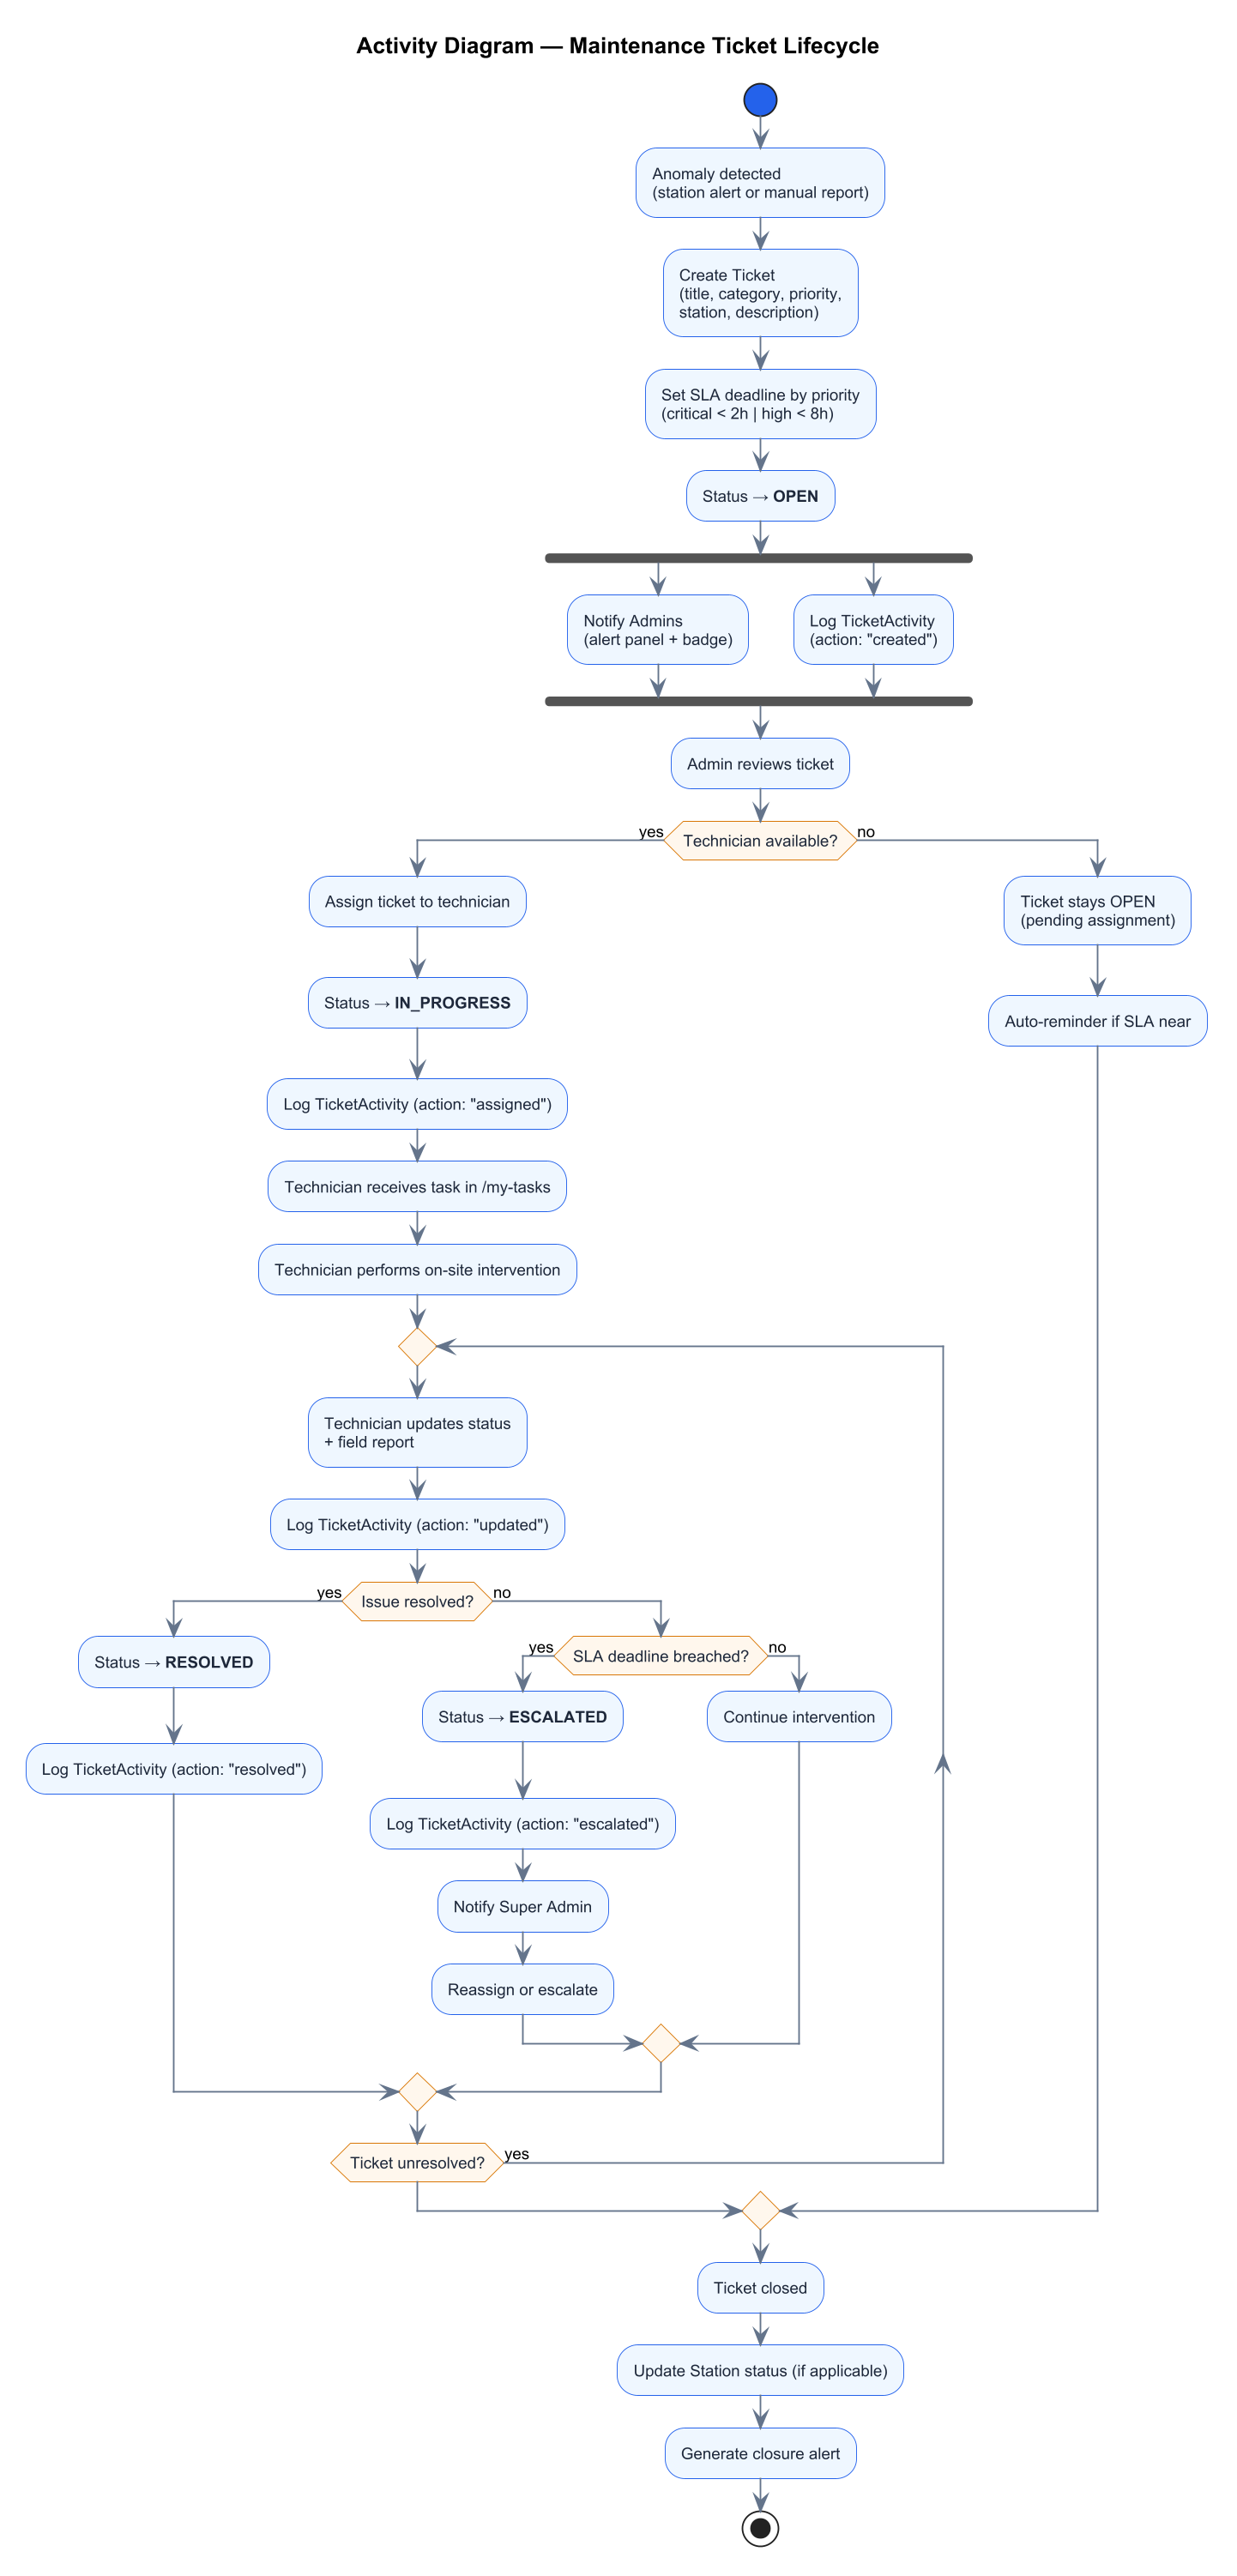
\includegraphics[width=0.62\textwidth, height=0.92\textheight, keepaspectratio]{../diagramme/ActivityTicket.png}
  \caption{Activity Diagram Maintenance Ticket Lifecycle}
  \label{fig:activity-ticket}
\end{figure}

\begin{figure}[htbp]
  \centering
  
\includegraphics[width=0.95\textwidth]{\detokenize{../../../Screens_4_chapter5/Task&Incidents}}
  \caption{Maintenance Ticket Module Ticket List and New Ticket Creation Form}
  \label{fig:tickets}
\end{figure}

\begin{figure}[htbp]
  \centering
  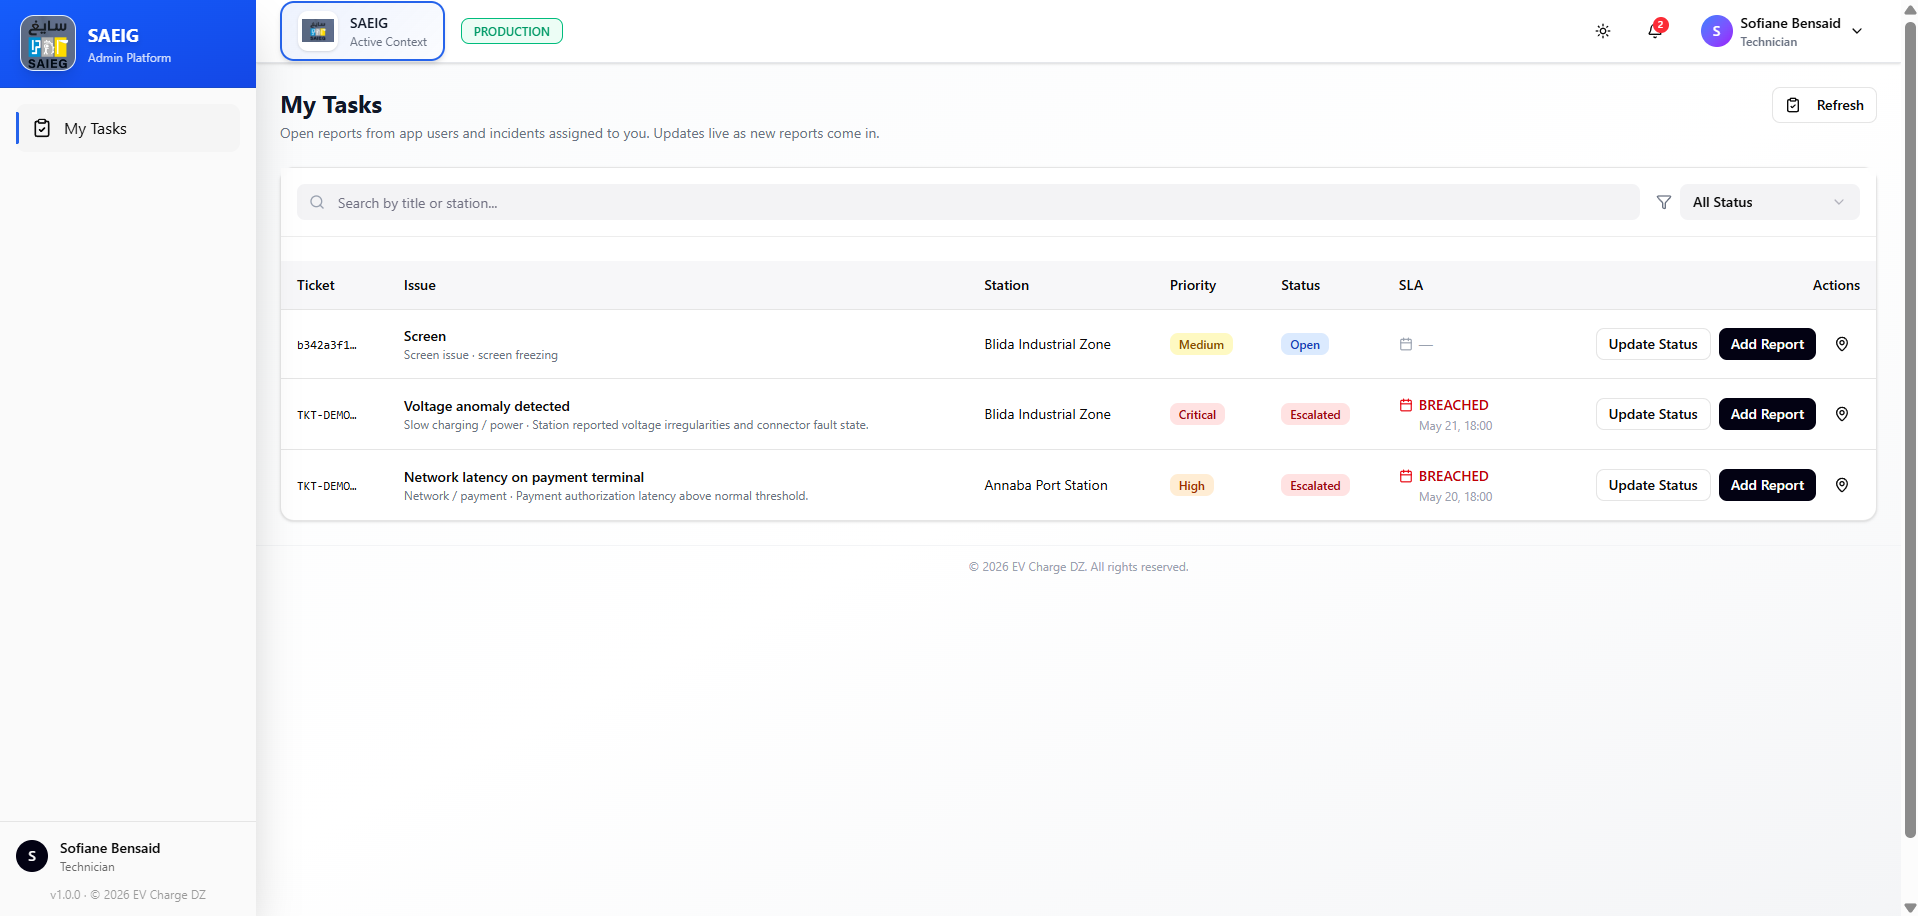
\includegraphics[width=0.72\textwidth]{../../../Screens_4_chapter5/MyTasks}
  \caption{My Tasks  Technician Personal Work Queue}
  \label{fig:my-tasks}
\end{figure}

% ──────────────────────────────────────────────────────────────────────────────
\section{User Management Module}

The User Management module is accessible by default to super\_admin accounts only. A
tenant\_admin account may also access it if a super\_admin explicitly grants the
\texttt{users\_view} and \texttt{users\_manage} privilege flags through the custom privilege
template. This allows operators to delegate user administration within their own tenant scope
without granting full cross-tenant authority. When creating a user, the administrator assigns:
a role (super\_admin, tenant\_admin, or technician), a tenant affiliation, and a privilege
template. As specified in Table~\ref{tab:privilege-matrix} (Section~4.5), each template
automatically assigns a predefined set of privilege flags that reflects the operator's
operational scope: \textit{standard\_admin} grants all thirteen flags (full platform access);
\textit{operations\_admin} covers infrastructure and session control but excludes billing~(9
flags); \textit{finance\_admin} provides read-only billing and reconciliation access~(8 flags);
and \textit{technician\_default} is scoped strictly to charge points and maintenance
tickets~(6 flags), omitting user data and billing in compliance with GDPR data-minimisation
requirements. The \textit{custom} template allows the administrator to manually select any
combination of individual privileges.

User accounts can be suspended (blocking login without deletion) and reactivated, providing
full lifecycle management of operator personnel.

\begin{figure}[htbp]
  \centering
  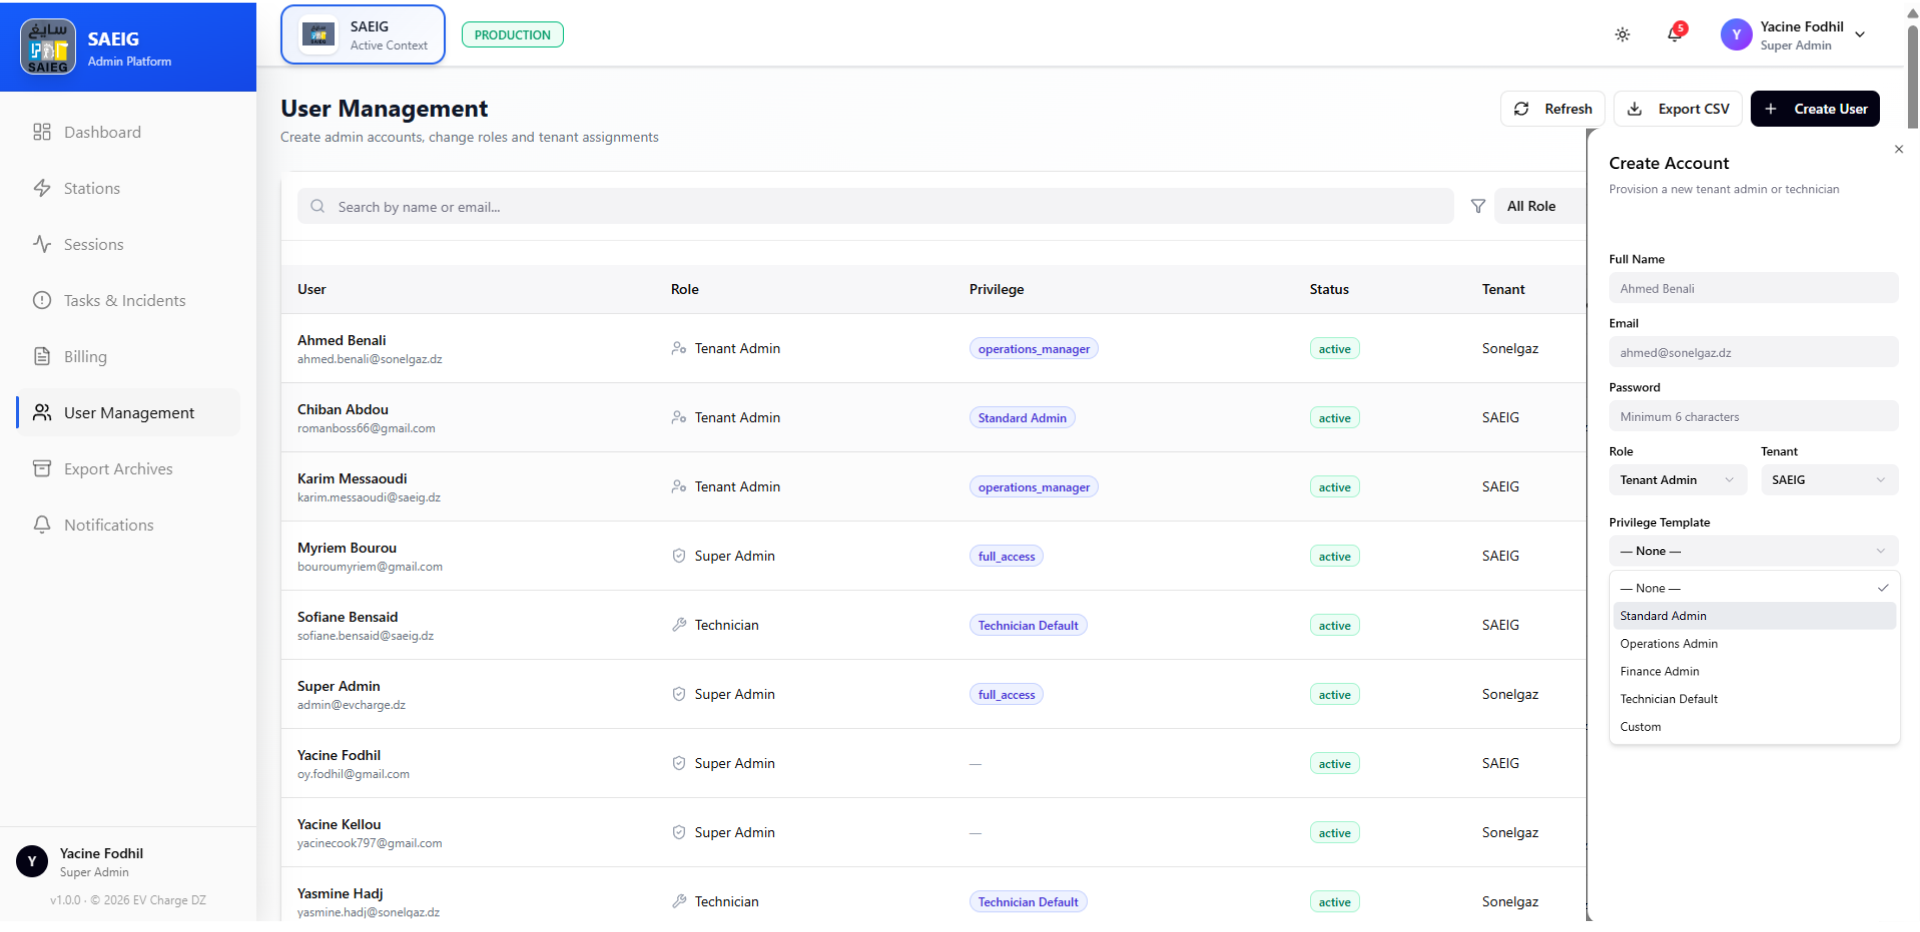
\includegraphics[width=0.95\textwidth]{../../../Screens_4_chapter5/usercreation}
  \caption{User Management Module User List and Account Creation Form}
  \label{fig:user-management}
\end{figure}

% ──────────────────────────────────────────────────────────────────────────────
\section{Push Notifications Module}

The Push Notifications module enables operators to broadcast real-time alerts to all
registered mobile app users within a tenant. A compose panel allows the sender to specify
a notification title, message body, an optional city filter (to target users in a specific
geographic area), and for super\_admin accounts a target tenant. Sent notifications
are recorded in a history panel displaying the delivery count, timestamp, and notification
type badge. The system supports five notification categories: \textit{station\_available},
\textit{station\_maintenance}, \textit{tariff\_change}, \textit{new\_station}, and
\textit{broadcast}. Operators may clear the history on demand using the dedicated button.

\begin{figure}[htbp]
  \centering
  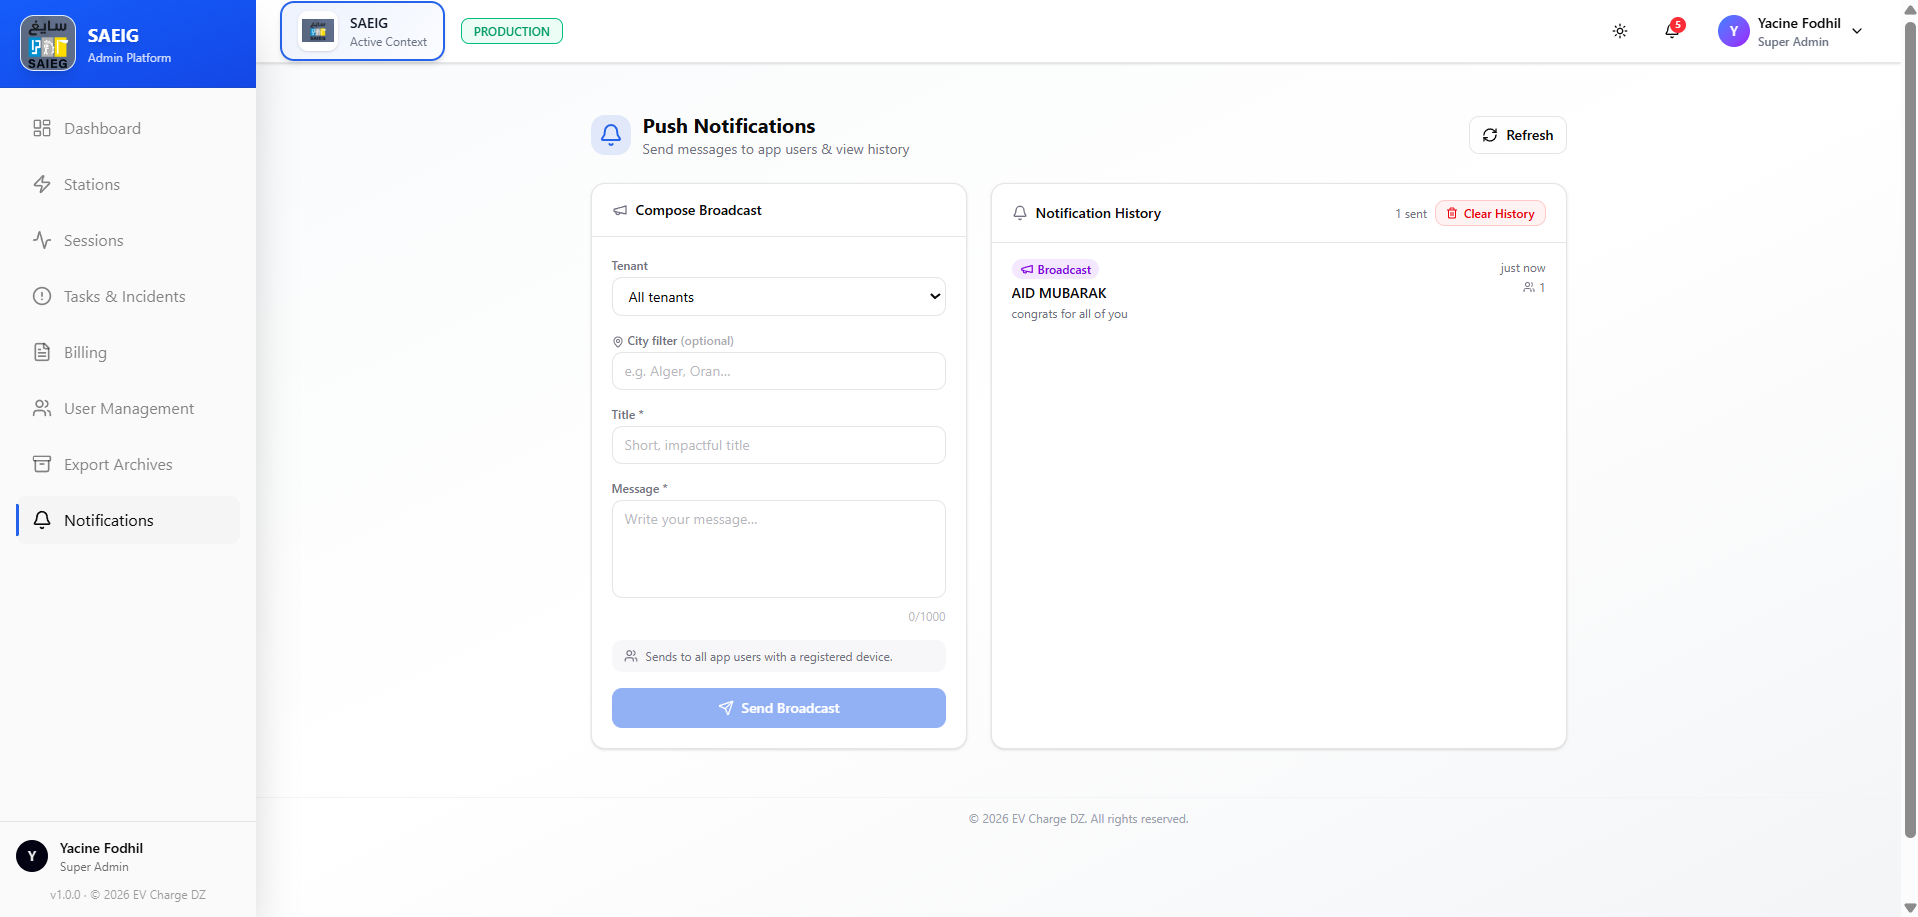
\includegraphics[width=0.95\textwidth]{../../../Screens_4_chapter5/notifications}
  \caption{Push Notifications Module Broadcast Composer and Notification History}
  \label{fig:notifications}
\end{figure}

% ──────────────────────────────────────────────────────────────────────────────
\section{Data Resilience and Offline Mode}

A key architectural decision is the platform's graceful degradation strategy. The frontend
checks for the presence of a backend API base URL at startup. When the backend is unreachable
(network failure or server downtime), the application falls back to data persisted in the
browser's \texttt{localStorage} and displays a prominent offline-mode notification banner.
This ensures operators retain read access to station lists, recent session records, and ticket
data even during connectivity interruptions.

% ──────────────────────────────────────────────────────────────────────────────
\section{Platform Summary}

\begin{table}[h!]
  \centering
  \caption{EV Charge Manager Platform Specification Summary}
  \label{tab:platform-summary}
  \renewcommand{\arraystretch}{1.3}
  \begin{tabular}{|>{\bfseries}p{4.5cm}|p{9cm}|}
    \hline
    Aspect                & Detail \\ \hline
    Platform Type         & Multi-tenant SaaS web application \\ \hline
    Target Market         & Algeria (Sonelgaz and SAEIG operators) \\ \hline
    Charging Protocol     & OCPP~1.6~\autocite{ocpp16_ed2} \\ \hline
    User Roles            & super\_admin, tenant\_admin, technician \\ \hline
    Granular Privileges   & 13 privilege types across 5 templates \\ \hline
    Authentication        & Email\,/\,password + OTP (2FA) + JWT~\autocite{rfc7519} \\ \hline
    Supported Connectors  & CCS2, CHAdeMO, Type~2 \\ \hline
    Payment Methods       & RFID card, CIB, e-payment \\ \hline
    Billing Currency      & Algerian Dinar (DZD) \\ \hline
    Frontend              & React~18 + TypeScript + Vite~\autocite{react_docs, vite_docs} \\ \hline
    Backend               & Node.js + Express.js~\autocite{nodejs_express} \\ \hline
    Database              & MySQL~8~\autocite{mysql_docs} \\ \hline
    Map                   & Leaflet / OpenStreetMap \\ \hline
    Offline Resilience    & localStorage fallback with graceful degradation \\ \hline
  \end{tabular}
\end{table}

% ──────────────────────────────────────────────────────────────────────────────
\section{Conclusion}

EV Charge Manager's implementation fulfils all ten functional requirements identified in
Chapter~3 and follows the architecture designed in Chapter~4. The eight operational
modules dashboard, station management, session monitoring, billing, maintenance tickets,
user management, push notifications, and offline resilience collectively deliver a
production-ready charging management solution adapted to Algeria's EV infrastructure context. The platform provides a
complete, locally adapted response to the gap identified in the introduction.

Chapter~6 extends the platform's scope by presenting the EVCharge Android mobile application,
the driver-facing companion that shares the same backend and database as the operator dashboard
described in this chapter.

%%%=============================================================================
%%  CHAPTER 6 — EVCHARGE MOBILE APPLICATION
%%%=============================================================================

\chapter{EVCharge : The Mobile Companion Application}

\section{Motivation and Objectives}

While EV Charge Manager provides network operators with a comprehensive web dashboard for
station management, session monitoring, and billing, the EV driver requires a dedicated mobile
interface. The EVCharge Android application was developed as the driver-facing complement to
the operator platform, closing the loop between infrastructure management and end-user
experience.

The application gives drivers the ability to locate nearby charging stations on an interactive
map, obtain turn-by-turn navigation directions to a selected station, report station problems
directly to operators, and receive real-time push notifications about station status changes and
tariff updates. All interactions are synchronised with the operator dashboard through a shared
backend infrastructure, ensuring that data visible to operators and data accessible to drivers
remain consistent at all times.

% ──────────────────────────────────────────────────────────────────────────────
\section{Technology Stack}

The application is developed in Kotlin targeting Android API~26 (Android~8.0 Oreo) as the
minimum supported version and API~34 (Android~14) as the target. Kotlin is Google's officially
recommended language for Android development, offering null safety, coroutine support, and full
interoperability with the Android SDK.

The user interface is built entirely with Jetpack Compose and Material~3, Google's modern
declarative UI toolkit for Android. Jetpack Compose eliminates XML layout files by defining UI
components as composable functions that react automatically to state changes a paradigm well
suited to the real-time nature of the application.

Table~\ref{tab:mobile-stack} summarises the complete technology stack used in the EVCharge
mobile application.

\begin{table}[h!]
  \centering
  \caption{EVCharge Mobile Application Technology Stack}
  \label{tab:mobile-stack}
  \renewcommand{\arraystretch}{1.3}
  \begin{tabular}{|>{\bfseries}p{4.5cm}|p{9cm}|}
    \hline
    Component           & Technology / Version \\ \hline
    Language            & Kotlin (JVM target~11) \\ \hline
    UI Framework        & Jetpack Compose + Material~3 (BOM~2024.09.00) \\ \hline
    Minimum SDK         & Android~8.0 Oreo (API~26) \\ \hline
    Target SDK          & Android~14 (API~34) \\ \hline
    Maps                & OSMDroid~6.1.18 (OpenStreetMap) \\ \hline
    HTTP Client         & Retrofit~2.9.0 + OkHttp~4.12.0 \\ \hline
    Push Notifications  & Firebase Cloud Messaging (FCM BOM~33.1.0) \\ \hline
    Real-Time Updates   & OkHttp WebSocket \\ \hline
    Asynchronous I/O    & Kotlin Coroutines~1.7.3 \\ \hline
  \end{tabular}
\end{table}

\begin{enumerate}
  \item \textbf{Kotlin + Jetpack Compose:} Modern Android development stack. Declarative UI,
        native coroutines, and null safety make it well suited to a real-time, network-driven
        application.
  \item \textbf{OSMDroid~6.1.18:} Android library for rendering OpenStreetMap tiles. Free,
        open-source, and consistent with the Leaflet/OpenStreetMap mapping used in the dashboard.
  \item \textbf{Retrofit~2 + OkHttp~4:} Industry-standard Android HTTP client stack. Retrofit
        provides a type-safe REST interface; OkHttp handles connection pooling, timeouts, and
        WebSocket connections.
  \item \textbf{Firebase Cloud Messaging:} Google's cross-platform push messaging service, used
        to deliver targeted notifications from the operator backend to registered driver devices.
\end{enumerate}

% ──────────────────────────────────────────────────────────────────────────────
\section{Application Architecture}

The application follows the Repository pattern, a standard Android architecture that separates
data-access logic from UI code. Each domain area authentication, stations, sessions, routes,
and tickets has a dedicated repository class that encapsulates all network calls and data
transformation. ViewModels expose observable state to the Compose UI layer, which reacts
declaratively to state changes without polling.

The data flow is: Compose screens observe ViewModel state, ViewModels call repository methods,
repositories call Retrofit API endpoints or the WebSocket manager, and responses propagate back
as Kotlin Flow or Result objects. All network operations run on \texttt{Dispatchers.IO}, keeping
the main thread free for UI rendering.

\begin{sloppypar}
Network configuration is centralised in \texttt{ServerConfig}, which defines the backend host,
port~3001, HTTP base URL, and WebSocket URL. \texttt{ApiClient} builds the Retrofit instance
with an OkHttp logging interceptor and a Gson converter. \texttt{ApiService} declares all REST
endpoint signatures as suspend functions, enabling direct use from coroutines without callback
boilerplate.
\end{sloppypar}

% ──────────────────────────────────────────────────────────────────────────────
\section{App-Dashboard Integration}

The most important architectural characteristic of EVCharge is that it shares the same
Node.js/Express backend server and the same MySQL database with the operator web dashboard.
This single-backend design ensures that data created by drivers charging sessions started
from the app, maintenance tickets submitted from the app is immediately visible to operators
on the dashboard, and vice versa.

\subsection{Shared Backend, Separated API Routes}

The server exposes two logically separate sets of API routes, each designed for its respective
client. Dashboard routes are authenticated with operator JWT tokens and subject to role-based
access control. Mobile app routes use driver JWT tokens and offer a simpler, consumer-oriented
interface. Table~\ref{tab:mobile-api} presents the mobile-specific API surface.

\begin{table}[h!]
  \centering
  \caption{Mobile App API Routes}
  \label{tab:mobile-api}
  \renewcommand{\arraystretch}{1.3}
  \begin{tabular}{|>{\bfseries}p{1.6cm}|p{5.5cm}|p{6.3cm}|}
    \hline
    Method  & Endpoint                       & Description \\ \hline
    POST    & /api/app/auth/register         & Driver account creation (email, password, full name) \\ \hline
    POST    & /api/app/auth/login            & Driver login --- returns JWT with 7-day validity \\ \hline
    POST    & /api/app/auth/fcm-token        & Register device FCM token for push notifications \\ \hline
    GET     & /api/app/stations              & Public list of all stations with GPS coordinates \\ \hline
    GET     & /api/app/stations/:id          & Single station details (connectors, price, status) \\ \hline
    GET     & /api/app/sessions              & Driver session history (paginated) \\ \hline
    POST    & /api/app/sessions              & Start a charging session at a station \\ \hline
    PATCH   & /api/app/sessions/:id          & Stop an active charging session \\ \hline
    POST    & /api/app/tickets               & Report a station problem as a maintenance ticket \\ \hline
    GET     & /api/app/route                 & ORS routing proxy --- returns GeoJSON driving route \\ \hline
  \end{tabular}
\end{table}

\subsection{Authentication Difference}

Dashboard operators complete a two-factor authentication flow: email/password followed by a
One-Time Password sent to their registered email address, after which a JWT is issued. This
two-factor requirement reflects the privileged nature of operator access to station management,
billing, and user data.

\begin{sloppypar}
Driver accounts authenticate with email and password only, without OTP verification. Drivers
are consumers managing their own sessions and have no access to operator data. Passwords are
hashed server-side with bcrypt at a cost factor of~12. The resulting JWT has a 7-day validity
and is stored in Android \texttt{SharedPreferences}. Every authenticated API request includes
the token as an \texttt{Authorization: Bearer} header.
\end{sloppypar}

% ──────────────────────────────────────────────────────────────────────────────
\section{Interactive Station Map}

\begin{sloppypar}
The map screen is the primary interface of the application. On launch, it calls the public
endpoint \texttt{GET /api/app/stations} and renders each returned station as a colour-coded
marker on an OSMDroid map backed by OpenStreetMap tiles the same tile provider used by the
Leaflet map in the operator dashboard.
\end{sloppypar}

Marker colour encodes operational status: green for \textit{available}, orange for
\textit{charging}, red for \textit{offline} or \textit{fault}, and grey for
\textit{maintenance}. This visual encoding is consistent with the status chip colours used in
the dashboard station table, giving both operators and drivers the same semantic colour
vocabulary.

Tapping a marker opens a \texttt{StationCard} bottom sheet displaying the station name,
address, operational status, maximum power in kilowatts, charging price in Algerian Dinars per
kilowatt-hour, supported connector types (CCS2, CHAdeMO, or Type~2), number of available
connectors out of the total, and an estimated charging time. From this card the driver can
launch navigation or initiate a charging session.

Station data is refreshed in real time by the WebSocket connection described in
Section~\ref{sec:mobile-websocket}: when an operator changes a station status on the dashboard,
the map marker updates on the driver device without requiring a manual refresh.

\begin{figure}[htbp]
  \centering
  \subcaptionbox{Station map with colour-coded markers\label{fig:screen-map}}[0.30\textwidth]{%
    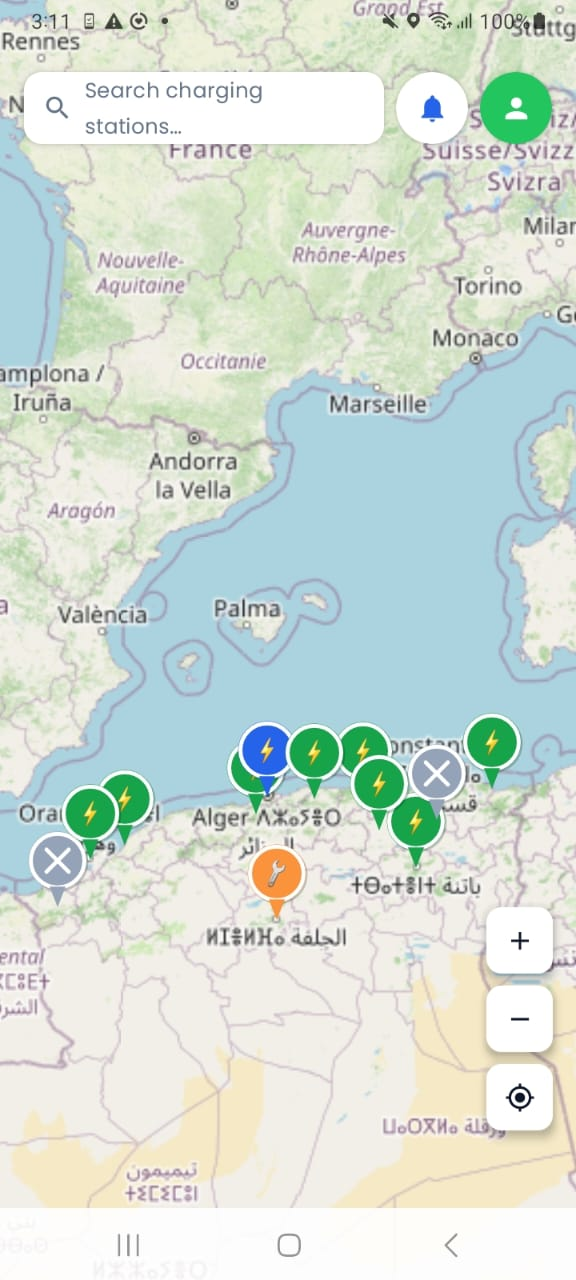
\includegraphics[width=0.30\textwidth,keepaspectratio]{../diagramme/screens/map_screen.jpg}}
  \hfill
  \subcaptionbox{Station search with live results\label{fig:screen-search}}[0.30\textwidth]{%
    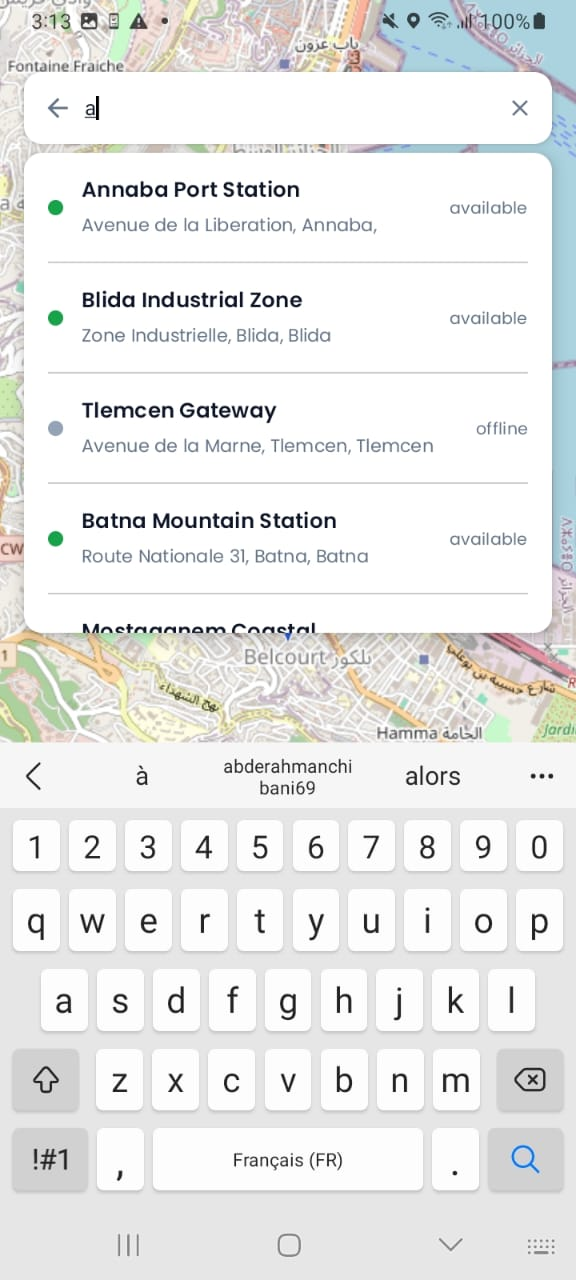
\includegraphics[width=0.30\textwidth,keepaspectratio]{../diagramme/screens/search_bar.jpg}}
  \hfill
  \subcaptionbox{StationCard bottom sheet\label{fig:screen-stationcard}}[0.30\textwidth]{%
    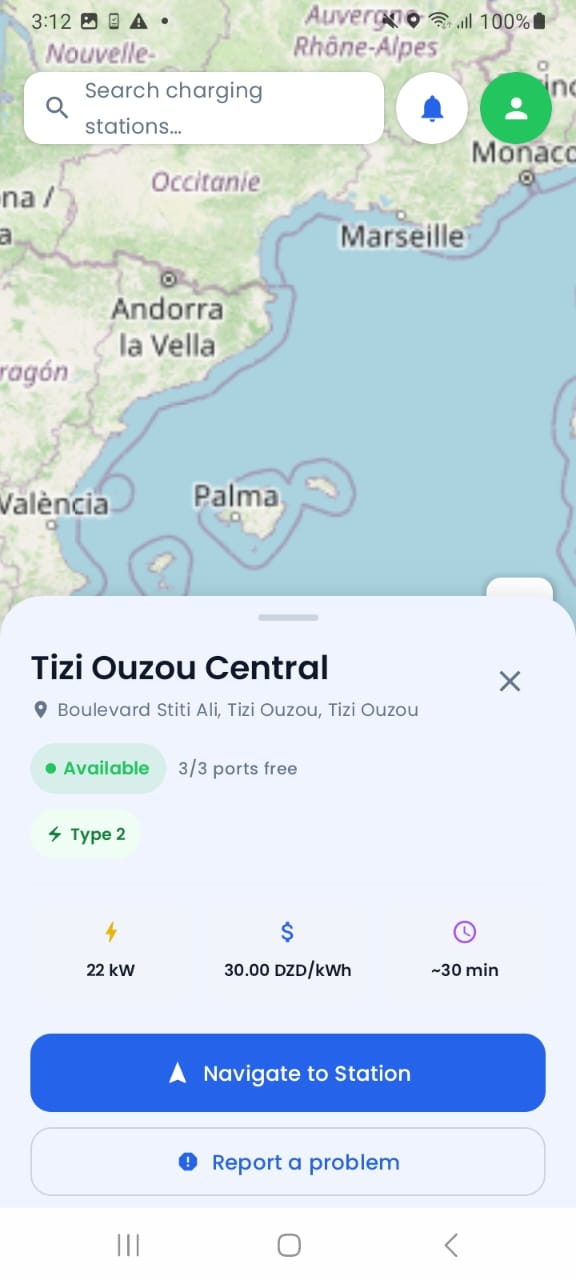
\includegraphics[width=0.30\textwidth,keepaspectratio]{../diagramme/screens/station_card.jpg}}
  \caption{EVCharge --- Interactive Station Map interface}
  \label{fig:screens-map-group}
\end{figure}

% ──────────────────────────────────────────────────────────────────────────────
\section{Navigation with OpenRouteService}

When a driver selects a station and taps Navigate, the application requests a driving route
from OpenRouteService~(ORS), an open-source routing engine built on OpenStreetMap road data.
ORS computes turn-by-turn directions and returns them as a GeoJSON FeatureCollection containing
the route geometry and a structured list of navigation steps.

\subsection{The ORS Proxy Architecture}

\begin{sloppypar}
The ORS API is not called directly from the Android device. Instead, the request is proxied
through the shared backend server at the endpoint \texttt{GET /api/app/route}, which accepts
the start and end coordinates as query parameters, forwards them to the ORS API, and relays the
GeoJSON response to the app. This design keeps the ORS API key server-side, preventing its
exposure in the compiled APK, and allows the phone to operate even in environments where direct
access to external APIs is restricted.
\end{sloppypar}

\begin{sloppypar}
The proxy applies a 15-second timeout to the upstream ORS request. If the request times out or
ORS returns an error, the server responds with an HTTP~502 or~504 status code, which the
\texttt{RouteRepository} translates into a \texttt{Kotlin Result.failure} for the ViewModel to
handle gracefully.
\end{sloppypar}

\subsection{Route Parsing and Display}

\begin{sloppypar}
The \texttt{RouteRepository} parses the GeoJSON response into a \texttt{RouteResult} data class
containing: a list of \texttt{GeoPoint} objects forming the polyline drawn on the OSMDroid map;
a list of \texttt{NavStep} objects each carrying a human-readable instruction, distance in
metres, duration in seconds, and an ORS maneuver type code (0\,=\,depart, 1\,=\,turn left,
2\,=\,turn right, 5\,=\,slight left, 6\,=\,slight right, 7\,=\,U-turn, 10\,=\,arrive); and
the total route distance and estimated duration displayed to the driver.

The \texttt{NavigationViewModel} manages step-by-step progression through the instruction list,
updating the currently active instruction as the driver advances along the route. The
\texttt{NavigationScreen} renders the OSMDroid map with the route polyline overlaid and a fixed
instruction panel at the bottom of the screen showing the current maneuver.
\end{sloppypar}

The complete navigation flow, from the driver tapping Navigate to step-by-step route
progression and error handling, is illustrated in Figure~\ref{fig:seq-navigation}.
Figure~\ref{fig:screen-navigation} shows the NavigationScreen on a real device, with the
ORS route polyline drawn over Algiers and the step instruction panel active at the bottom.

\begin{figure}[htbp]
  \centering
  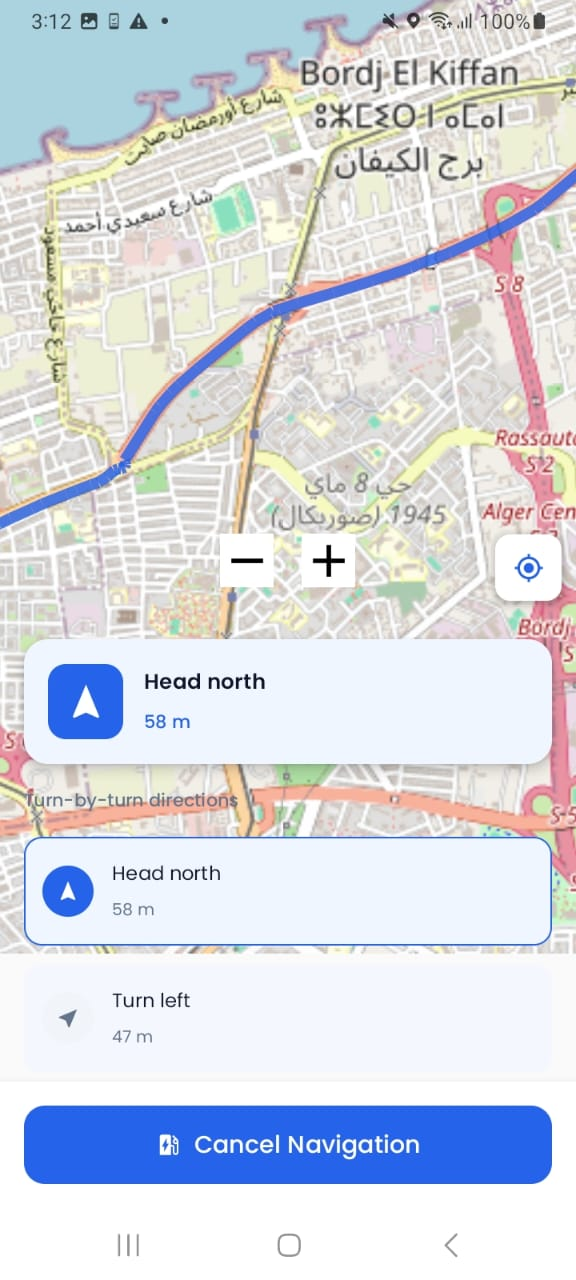
\includegraphics[width=0.44\textwidth,keepaspectratio]{../diagramme/screens/navigation_screen.jpg}
  \caption{NavigationScreen --- ORS route polyline and step-by-step instruction panel}
  \label{fig:screen-navigation}
\end{figure}

\begin{figure}[p]
  \centering
  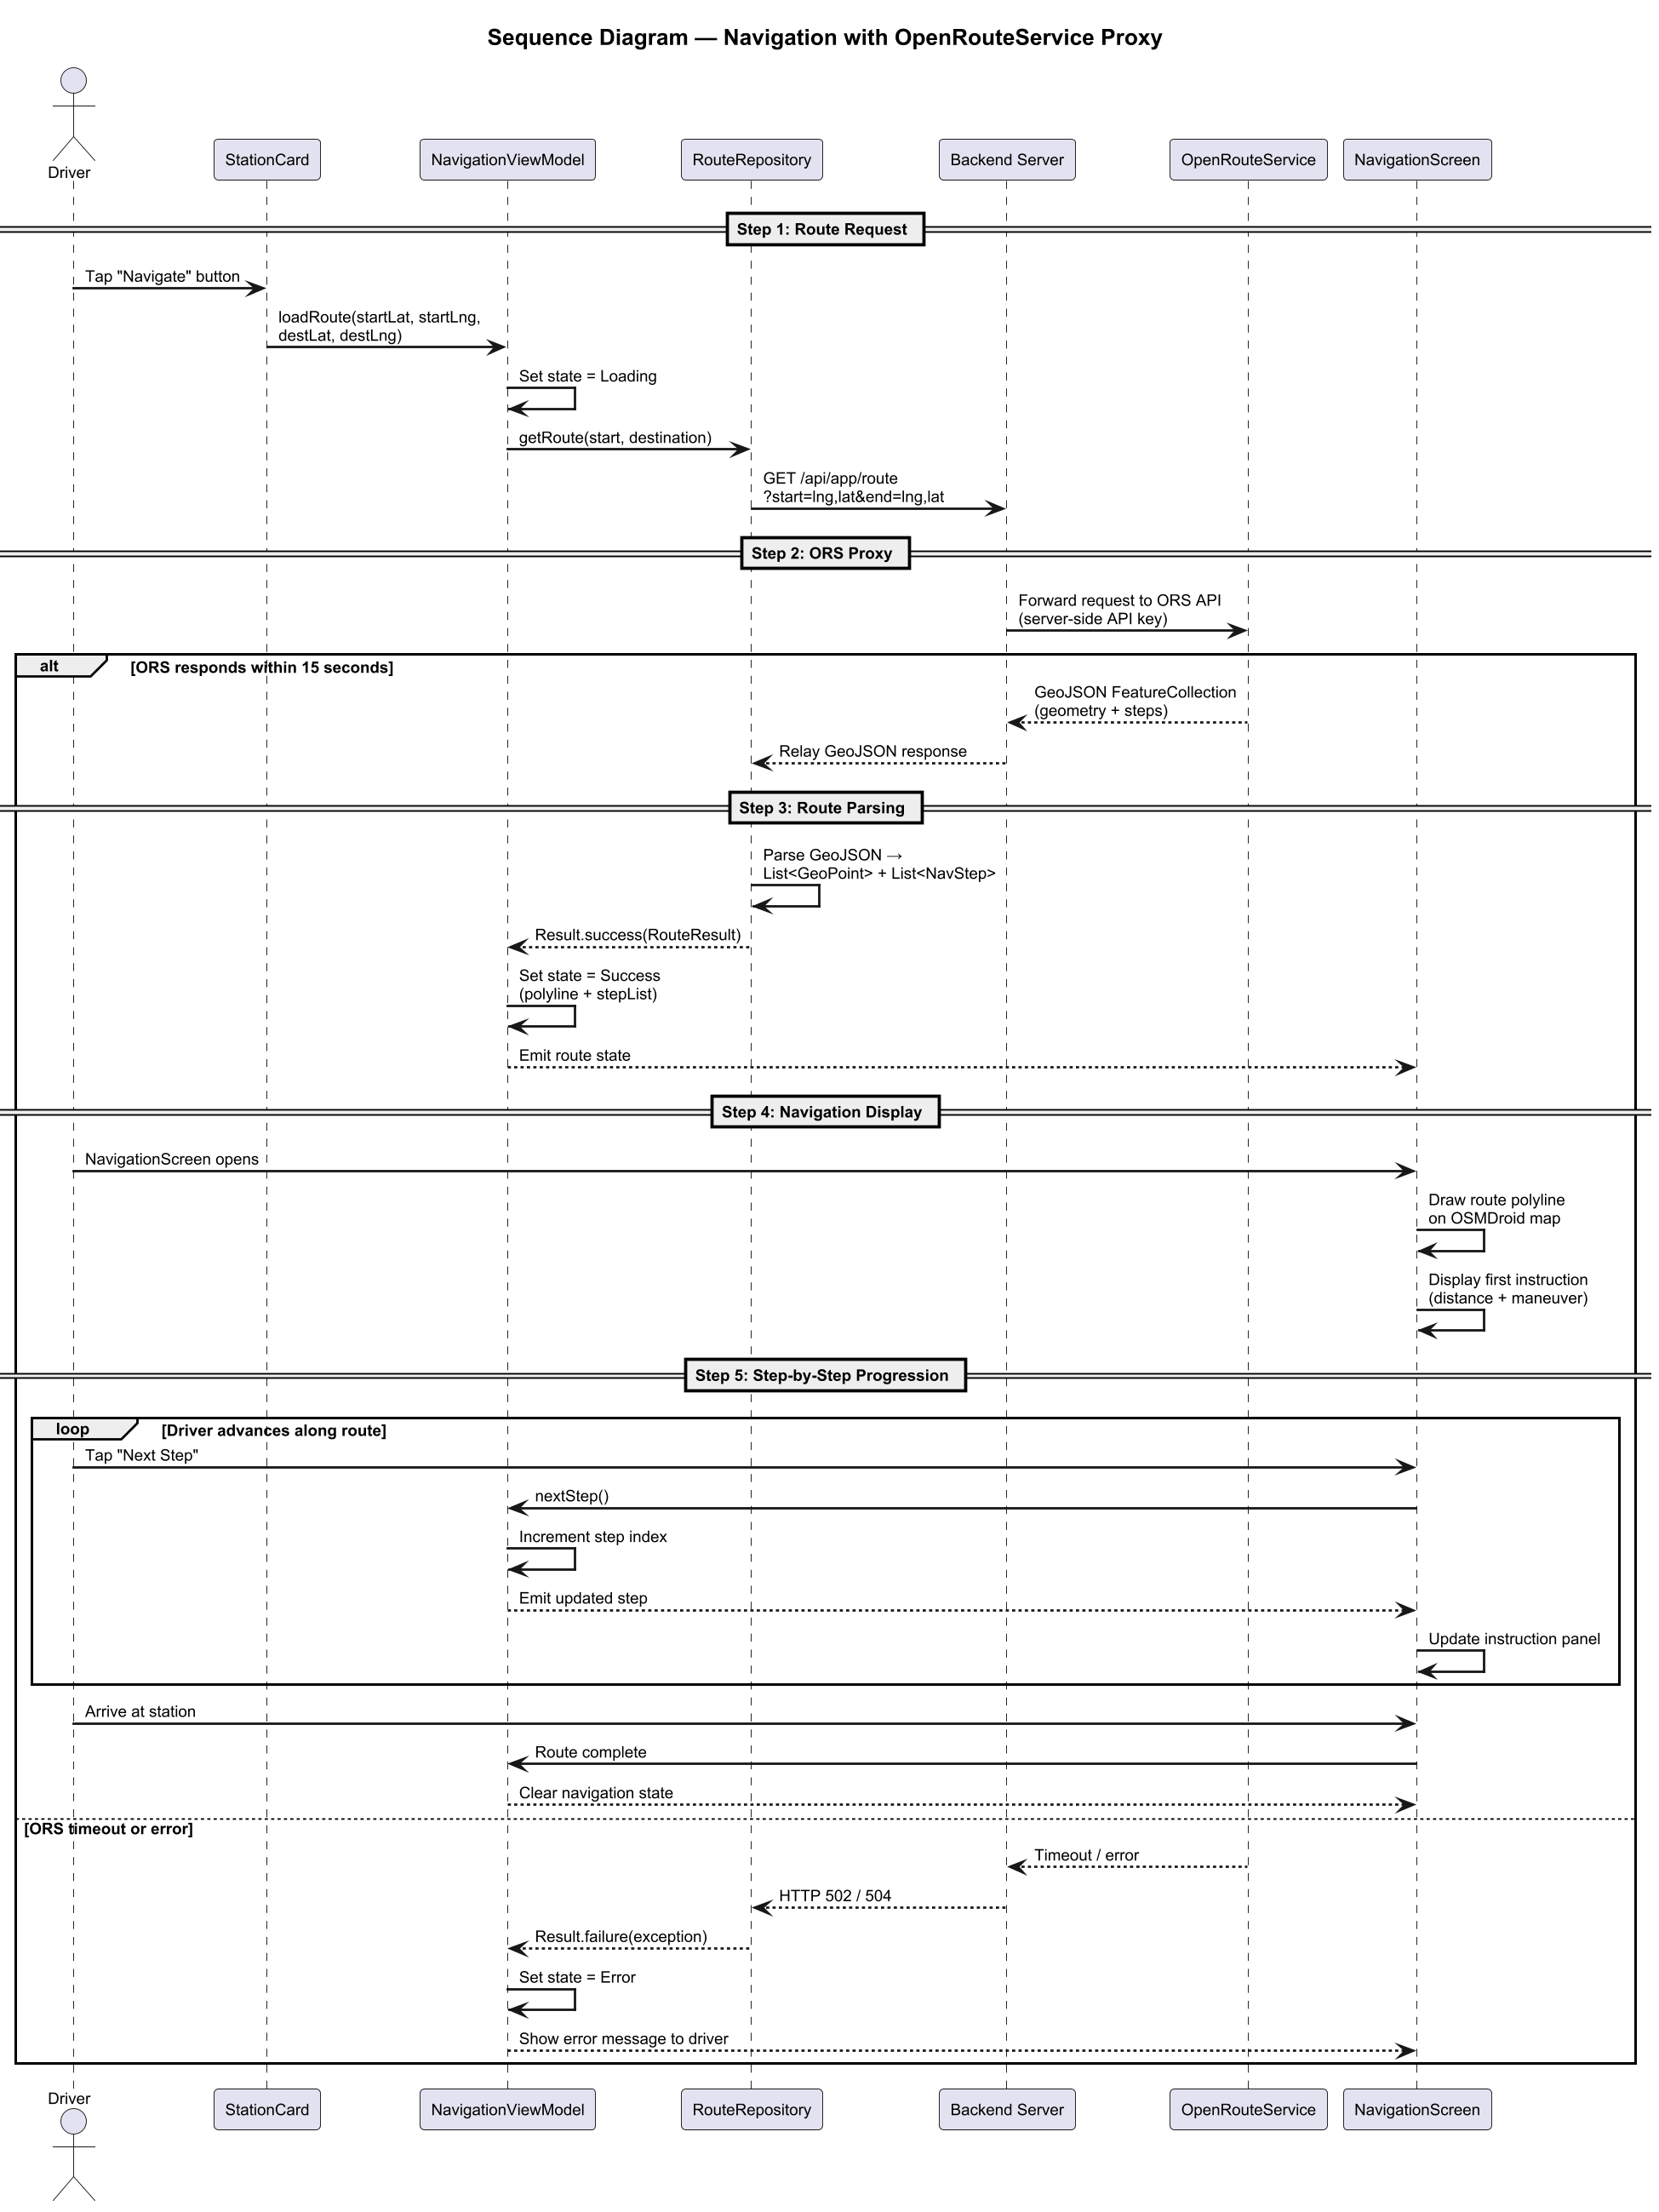
\includegraphics[width=\textwidth, height=0.92\textheight, keepaspectratio]{../diagramme/SeqNavigation.png}
  \caption{Sequence Diagram --- Navigation with OpenRouteService Proxy}
  \label{fig:seq-navigation}
\end{figure}

% ──────────────────────────────────────────────────────────────────────────────
\section{Real-Time Station Updates via WebSocket}
\label{sec:mobile-websocket}

\begin{sloppypar}
The application maintains a persistent WebSocket connection to the backend at
\texttt{ws://[host]:3001/ws} from the moment the map screen is active. When a dashboard
operator changes a station status for example, toggling a station into maintenance mode
the server broadcasts a \texttt{station\_status\_update} message over this channel.

The \texttt{WebSocketManager} singleton handles the connection lifecycle using OkHttp's
WebSocket API. Incoming messages are parsed from JSON and emitted to a
\texttt{MutableSharedFlow}. The \texttt{MapScreen} collects this flow, which triggers a Compose
recomposition that updates the affected marker colour without requiring a full data reload.

Auto-reconnect logic is implemented in the connection failure callback: if the WebSocket drops,
the manager schedules a reconnect attempt after 5 seconds. This makes the real-time update
mechanism resilient to brief network interruptions.

This WebSocket channel is shared with the operator dashboard, which uses the same server-side
broadcast mechanism via the \texttt{useLiveEvents} React hook. Both the operator and the driver
therefore see status changes propagate simultaneously without polling.
\end{sloppypar}

% ──────────────────────────────────────────────────────────────────────────────
\section{Firebase Cloud Messaging}

Firebase Cloud Messaging~(FCM) is the bridge between the operator dashboard and the driver
application for asynchronous push notifications. It allows the backend to reach any registered
Android device instantly, even when the application is in the background or closed.

\subsection{Token Registration Flow}

\begin{sloppypar}
When the driver logs in, the Firebase SDK generates a device-specific FCM token. The
\texttt{EvChargeMessagingService} class, which extends \texttt{FirebaseMessagingService},
intercepts the token via the \texttt{onNewToken} callback and calls
\texttt{POST /api/app/auth/fcm-token} to register it with the backend. The server stores the
token in the \texttt{app\_users.fcm\_token} database column. The callback also fires when FCM
rotates the token automatically, ensuring the stored value remains current.

On the backend side, the Firebase Admin SDK is initialised with a service account. When an
event requires driver notification, the \texttt{fcmHelper} module queries the database for
relevant FCM tokens and dispatches messages using
\texttt{admin.messaging().sendEachForMulticast()}.
\end{sloppypar}

\subsection{Notification Types and Targeting}

Five notification types are dispatched from the backend, each using a different targeting
strategy to ensure relevance. Table~\ref{tab:fcm-types} summarises the notification types,
their triggers, and their targeting scope.

\begin{table}[h!]
  \centering
  \caption{FCM Notification Types}
  \label{tab:fcm-types}
  \renewcommand{\arraystretch}{1.3}
  \begin{tabular}{|>{\ttfamily\small}p{4cm}|p{4.5cm}|p{5cm}|}
    \hline
    \normalfont\textbf{Type} & \textbf{Trigger} & \textbf{Target Audience} \\ \hline
    station\_available    & Station returns to available status   & Users who charged there in the last 30 days \\ \hline
    station\_maintenance  & Operator sets station to maintenance  & Users who charged there in the last 30 days \\ \hline
    tariff\_change        & Operator updates charging price       & Users who charged there in the last 60 days \\ \hline
    new\_station          & Operator adds a new station           & All users in the station city \\ \hline
    broadcast             & Operator sends a manual announcement  & All registered app users (optional city filter) \\ \hline
  \end{tabular}
\end{table}

\begin{sloppypar}
On the Android side, \texttt{EvChargeMessagingService} routes each incoming message to the
appropriate notification channel: \texttt{station\_updates} (high priority) for station status
events, \texttt{tariff\_updates} for price changes, and \texttt{announcements} for broadcasts
and new station alerts. Each notification is also persisted to \texttt{SharedPreferences} as a
JSON entry and displayed in the in-app Notifications screen, allowing drivers to review past
alerts.
\end{sloppypar}

The complete FCM flow covering token registration and notification dispatch is illustrated
in Figure~\ref{fig:seq-fcm}. Figure~\ref{fig:screen-notifications} shows the in-app
\texttt{NotificationsScreen} displaying a received broadcast announcement.

\begin{figure}[htbp]
  \centering
  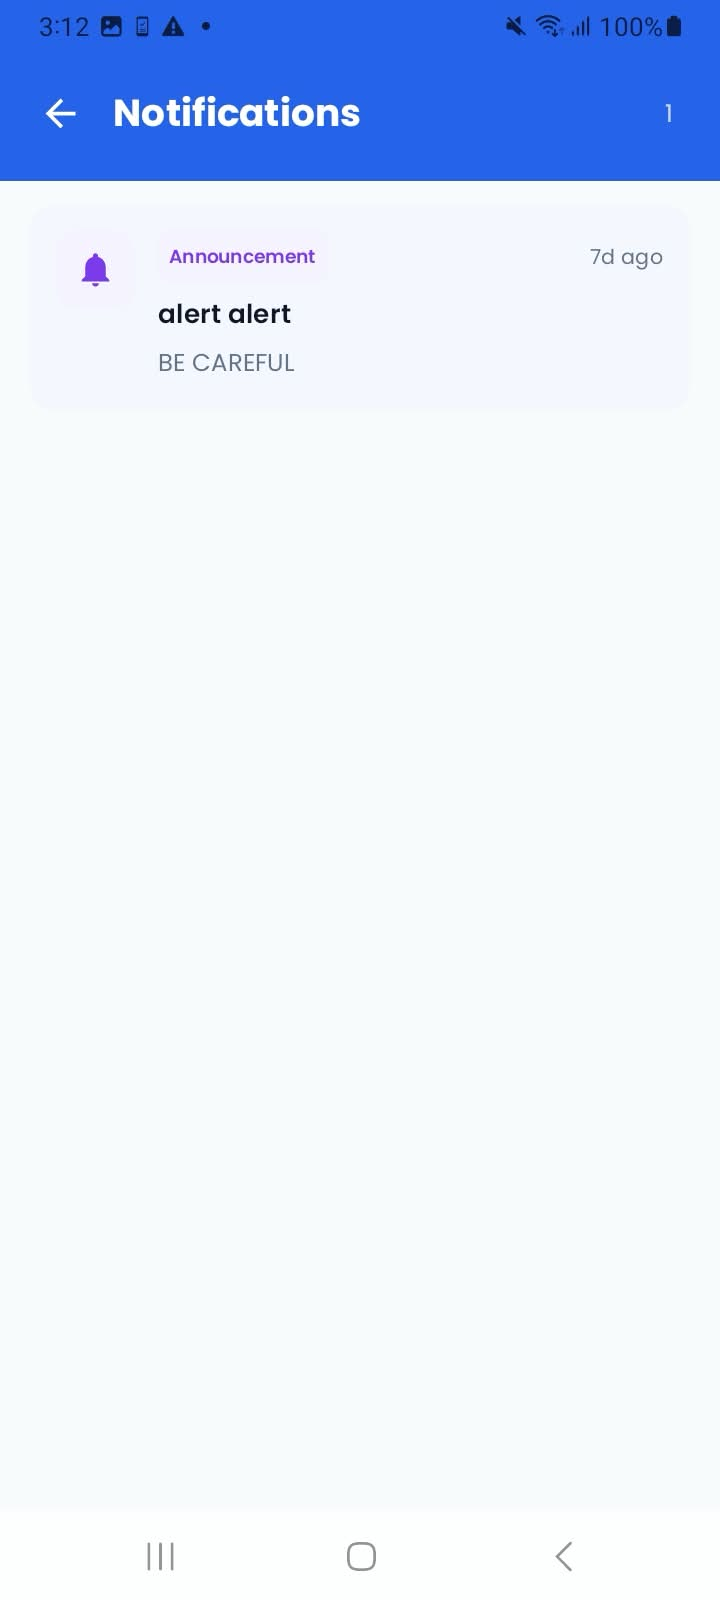
\includegraphics[width=0.44\textwidth,keepaspectratio]{../diagramme/screens/notification_screen.jpg}
  \caption{NotificationsScreen --- received FCM push notifications listed chronologically}
  \label{fig:screen-notifications}
\end{figure}

\begin{figure}[p]
  \centering
  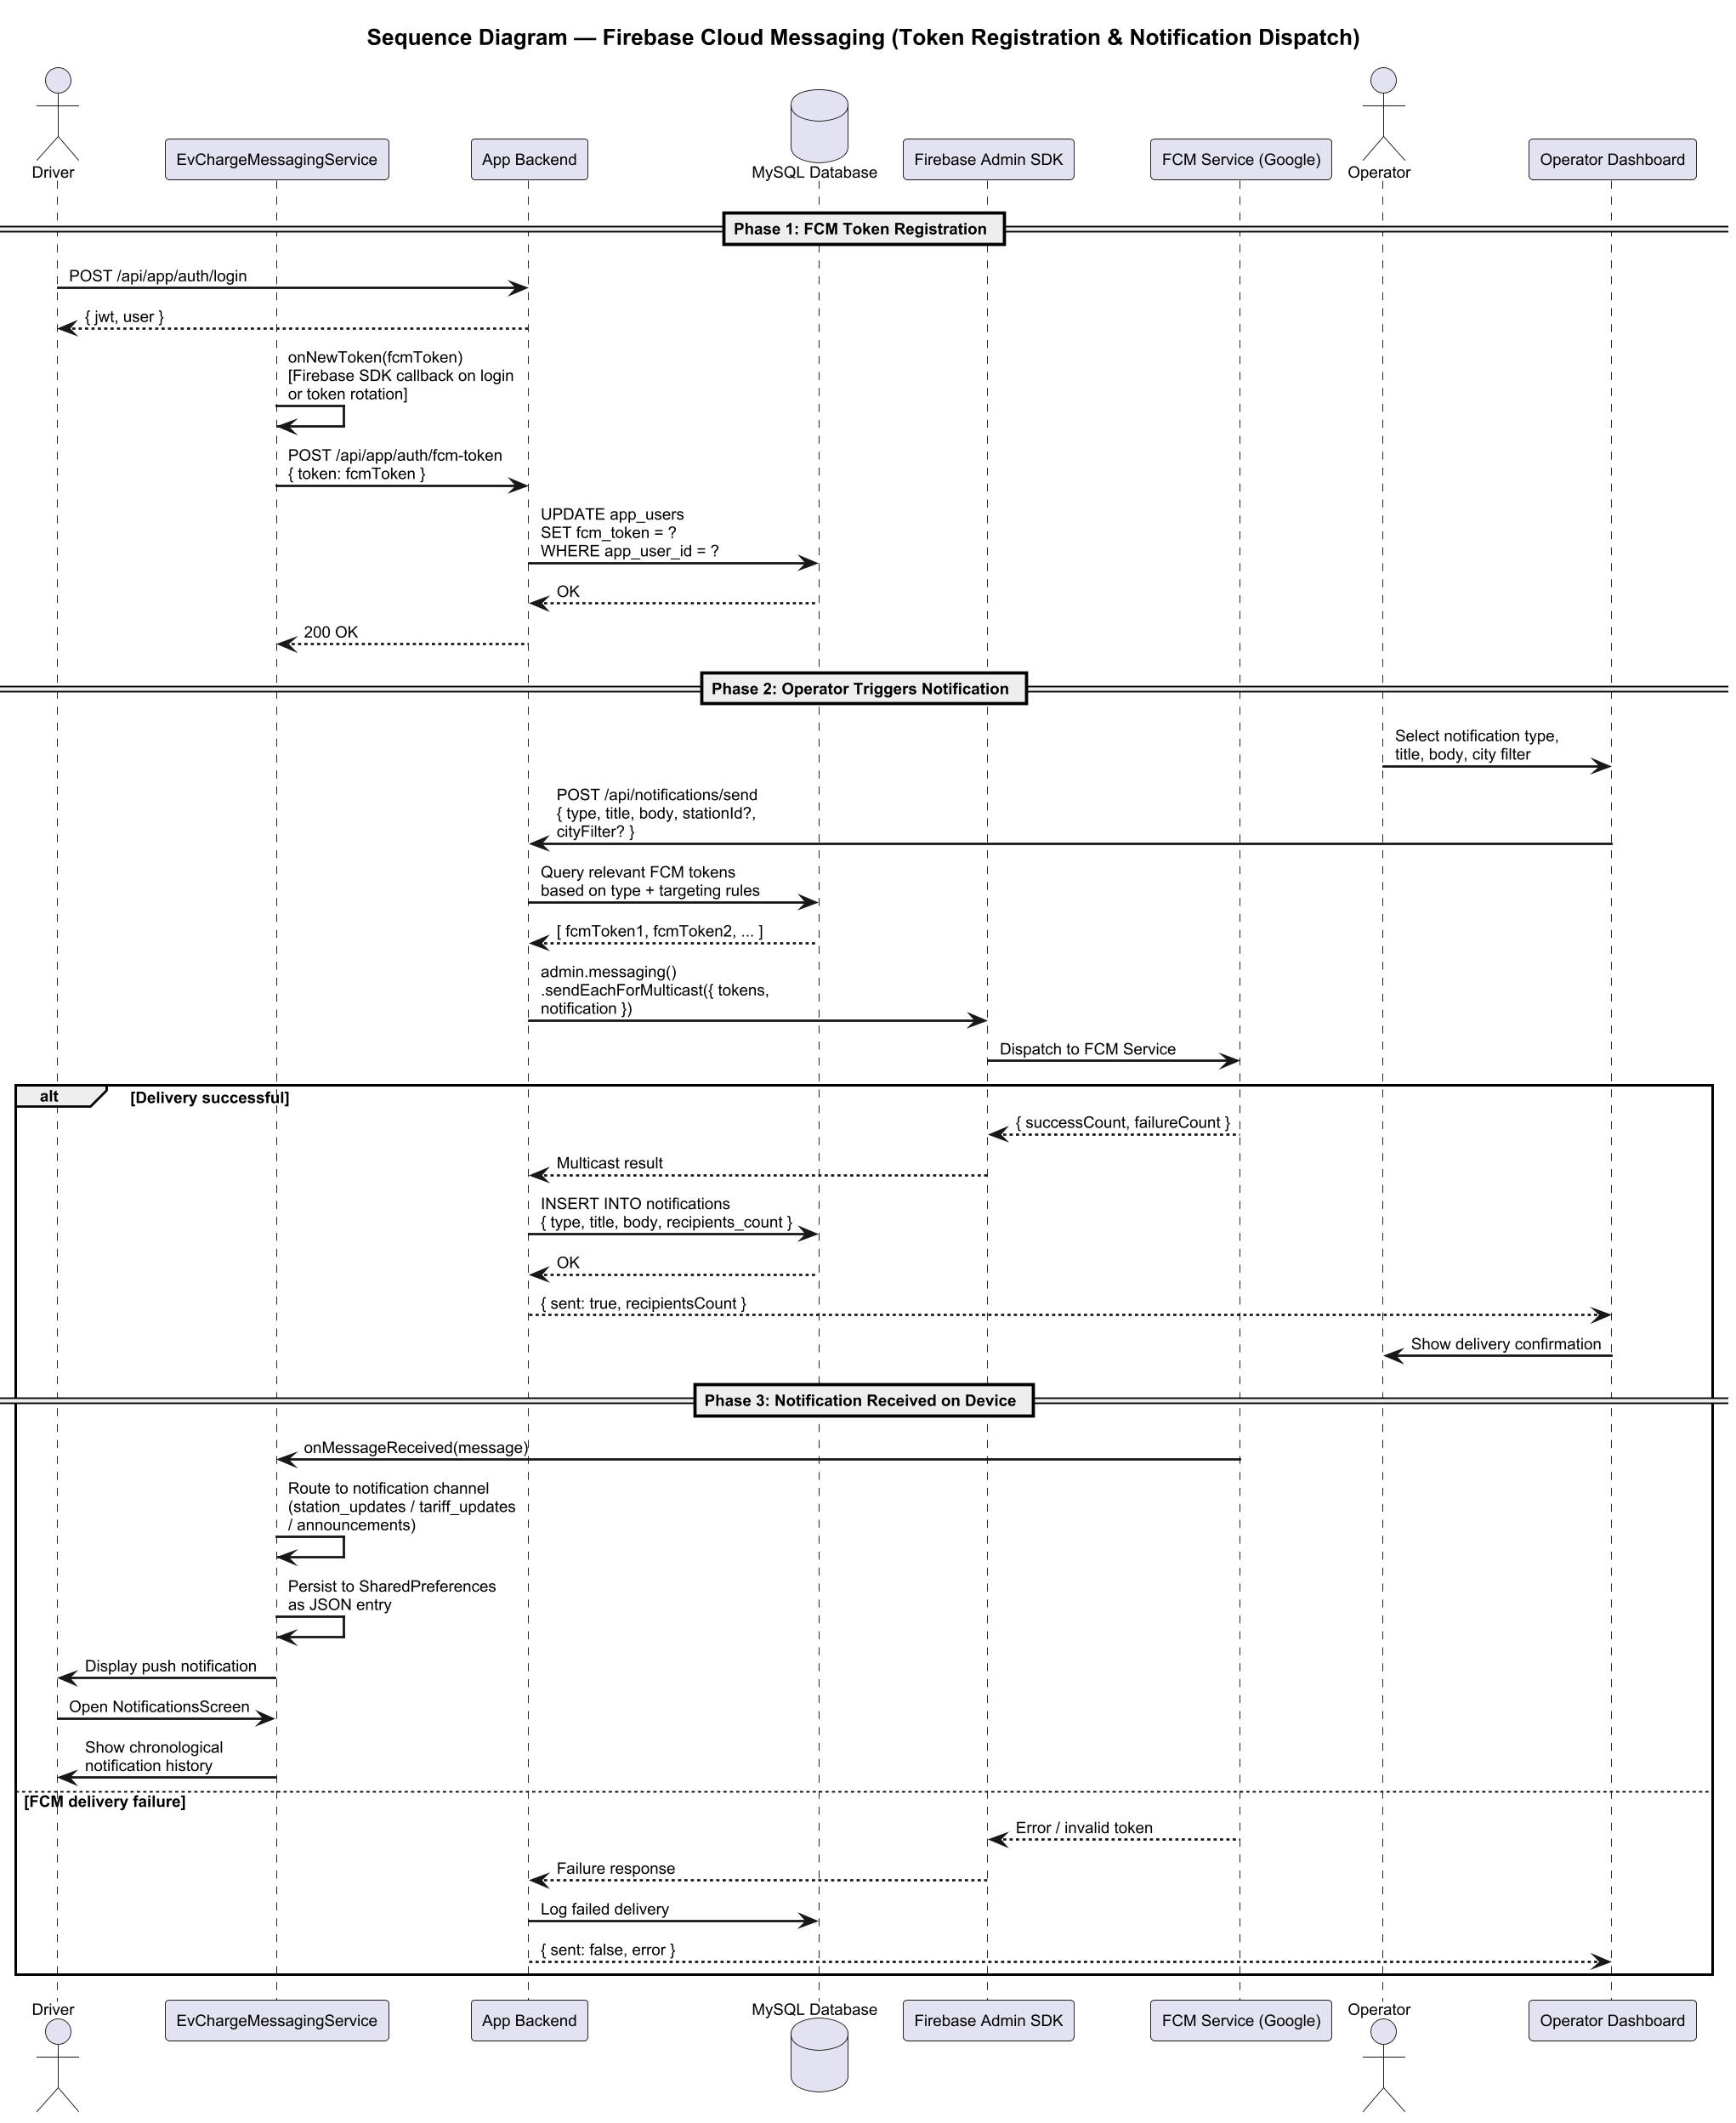
\includegraphics[width=\textwidth, height=0.92\textheight, keepaspectratio]{../diagramme/SeqFCM.png}
  \caption{Sequence Diagram --- Firebase Cloud Messaging (Token Registration \& Notification Dispatch)}
  \label{fig:seq-fcm}
\end{figure}

% ──────────────────────────────────────────────────────────────────────────────
\section{Charging Session Management}

\begin{sloppypar}
Drivers can start and stop charging sessions directly from the \texttt{StationCard} bottom
sheet. Starting a session calls \texttt{POST /api/app/sessions} with the selected station
identifier and the chosen payment method. The server validates station availability, creates a
record in the \texttt{charging\_sessions} table, and returns the session identifier, estimated
cost in DZD, and a status field.

Stopping a session calls \texttt{PATCH /api/app/sessions/\{session\_id\}} with the
\texttt{action} field set to \texttt{stop}. The server computes the final duration in minutes,
energy delivered in kWh, and the billed amount in DZD, closes the session record, and returns
these values for display to the driver.

Session records created through the mobile app are stored in the same
\texttt{charging\_sessions} database table accessed by the dashboard Session Monitoring Module.
Operators therefore see app-initiated sessions alongside RFID-initiated and CIB-initiated
sessions in a unified view, with the source identified by the \texttt{payment\_method} field.

Drivers can retrieve their session history via \texttt{GET /api/app/sessions}, which returns a
paginated list of past sessions with station name, connector type, start time, duration, energy
consumed, cost, and final status.
\end{sloppypar}

\begin{figure}[htbp]
  \centering
  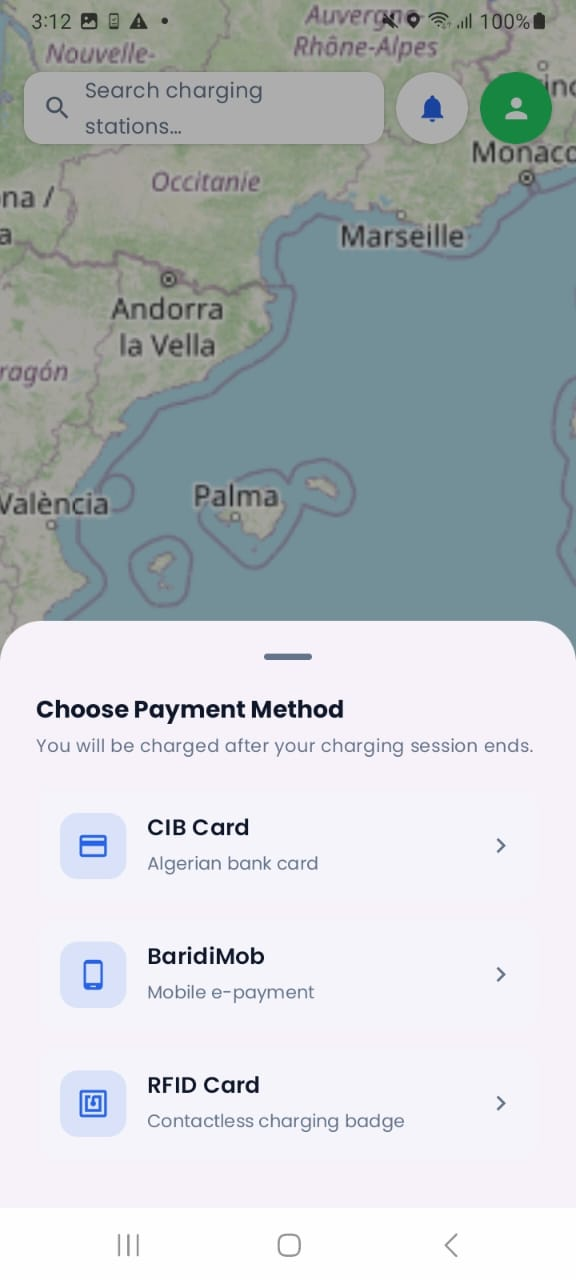
\includegraphics[width=0.44\textwidth,keepaspectratio]{../diagramme/screens/payment_method.jpg}
  \caption{Payment method selection --- CIB Card, BaridiMob, and RFID Card options}
  \label{fig:screen-payment}
\end{figure}

% ──────────────────────────────────────────────────────────────────────────────
\section{Problem Reporting}

\begin{sloppypar}
If a driver encounters a problem with a charging station, the \texttt{ReportProblemSheet}
bottom sheet allows them to submit a maintenance ticket directly from the application. The
driver selects the affected station and chooses a fault category from six options: power
failure, screen issue, charger fault, system failure, network issue, or scheduled maintenance.
An optional description field allows additional context.

The ticket is created via \texttt{POST /api/app/tickets} and is inserted into the same
\texttt{tickets} table used by the operator dashboard Ticket Management Module. The ticket
appears immediately in the operator ticket queue with the category and an activity log entry
recording its origin. Operators can then assign a technician, set an SLA deadline, and track
resolution as with any operator-generated ticket.
\end{sloppypar}

This mechanism creates a closed feedback loop: a driver identifies a problem in the field and
reports it in seconds; the operator is notified through the dashboard; a technician is assigned
and resolves the issue; the station returns to available status and drivers who used that
station recently receive an FCM push notification confirming availability.

\begin{figure}[htbp]
  \centering
  \subcaptionbox{Fault category selection\label{fig:report-a}}[0.44\textwidth]{%
    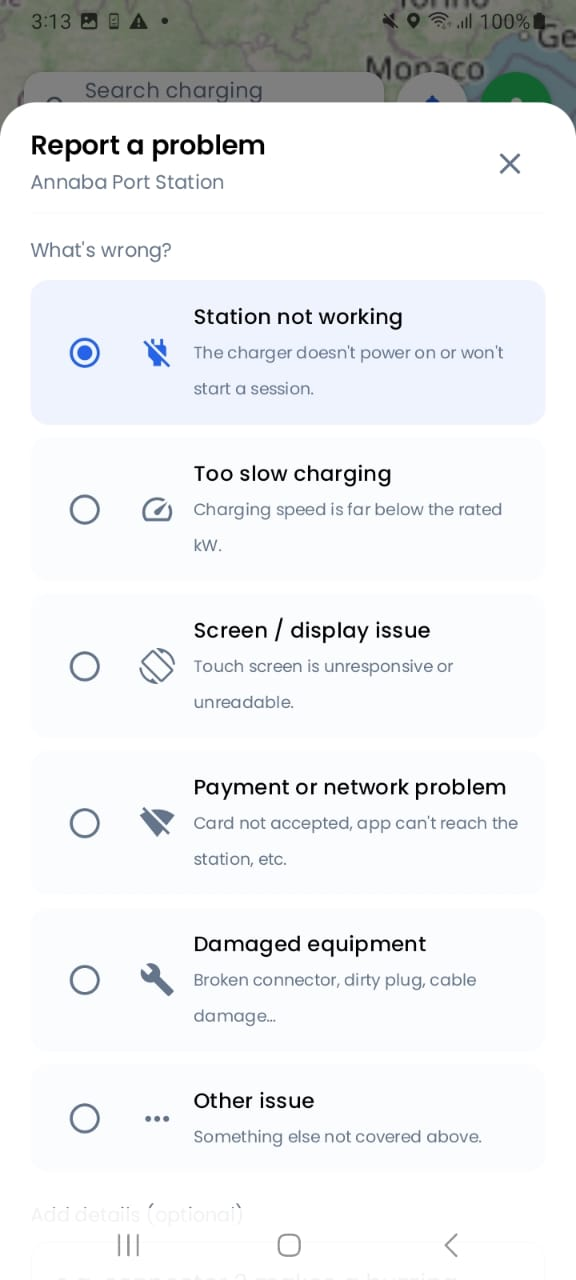
\includegraphics[width=0.44\textwidth,keepaspectratio]{../diagramme/screens/report_screen.jpg}}
  \hfill
  \subcaptionbox{Additional details and submission\label{fig:report-b}}[0.44\textwidth]{%
    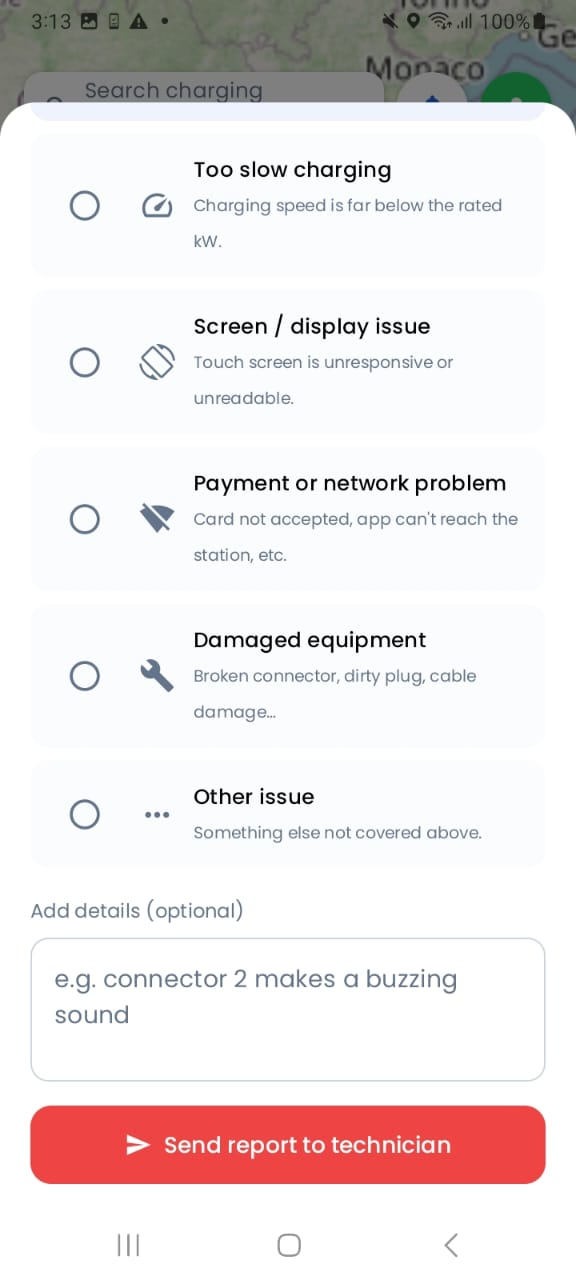
\includegraphics[width=0.44\textwidth,keepaspectratio]{../diagramme/screens/report_screen_2.jpg}}
  \caption{ReportProblemSheet --- fault category selection and ticket submission}
  \label{fig:screens-report}
\end{figure}

% ──────────────────────────────────────────────────────────────────────────────
\section{Application Screens Overview}

Table~\ref{tab:app-screens} summarises the screens implemented in the EVCharge application,
each corresponding to a source file in the \texttt{ui/screens} package.

\begin{table}[h!]
  \centering
  \caption{EVCharge Application  Screen Summary}
  \label{tab:app-screens}
  \renewcommand{\arraystretch}{1.3}
  \begin{tabularx}{\textwidth}{|>{\bfseries}p{4.5cm}|X|}
    \hline
    Screen                & Description \\ \hline
    SplashScreen          & Entry point: checks for a stored JWT and routes to login or map. \\ \hline
    LoginScreen           & Email and password authentication with a registration link. \\ \hline
    MapScreen             & OSMDroid map with colour-coded station markers and real-time WebSocket updates. \\ \hline
    StationCard           & Bottom sheet showing station details with Navigate and Start Session actions. \\ \hline
    NavigationScreen      & Turn-by-turn navigation with ORS route polyline and a step instruction panel. \\ \hline
    NotificationsScreen   & Chronological list of received FCM push notifications. \\ \hline
    ReportProblemSheet    & Bottom sheet for submitting a station fault report as a maintenance ticket. \\ \hline
  \end{tabularx}
\end{table}

\begin{figure}[htbp]
  \centering
  \subcaptionbox{Login screen\label{fig:screen-login}}[0.44\textwidth]{%
    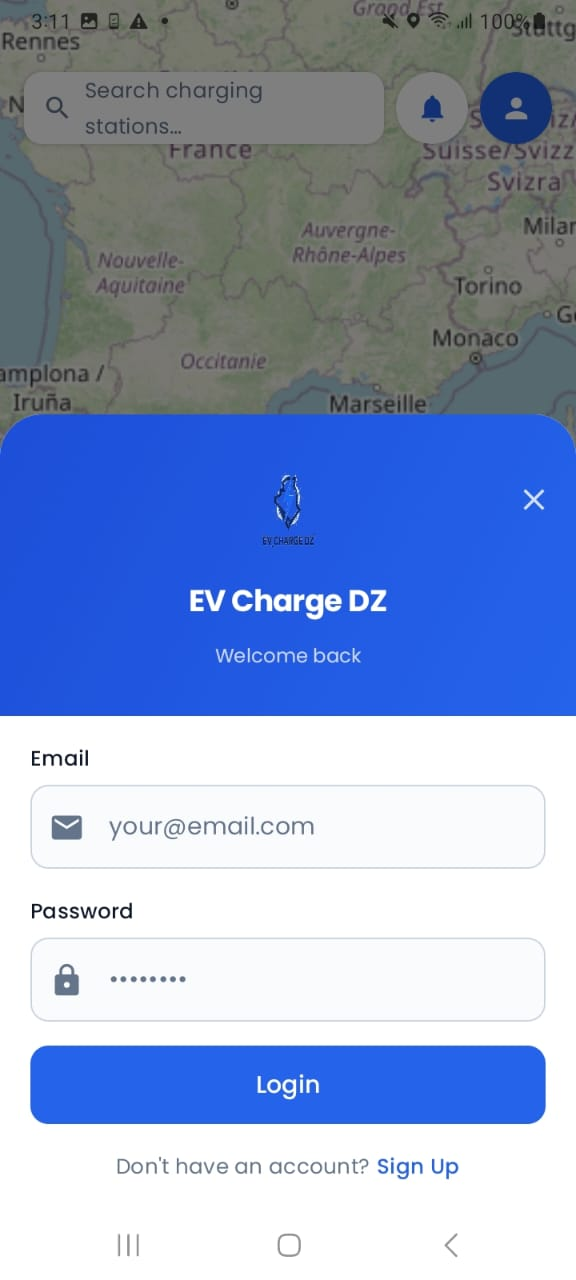
\includegraphics[width=0.44\textwidth,keepaspectratio]{../diagramme/screens/login_screen.jpg}}
  \hfill
  \subcaptionbox{Registration screen\label{fig:screen-signup}}[0.44\textwidth]{%
    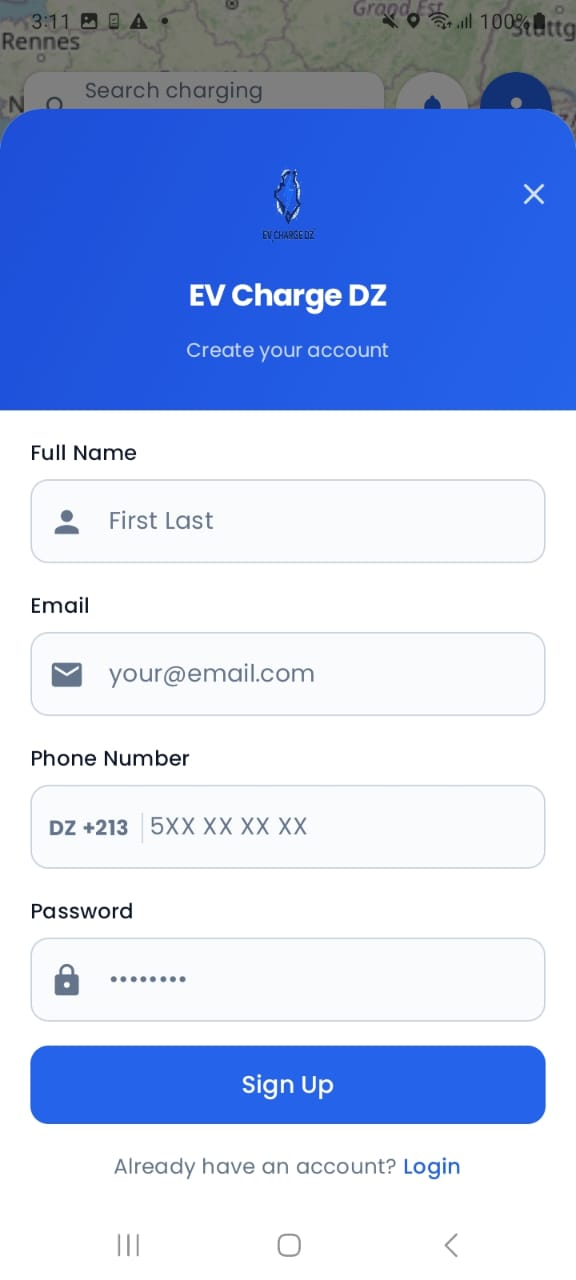
\includegraphics[width=0.44\textwidth,keepaspectratio]{../diagramme/screens/signup_screen.jpg}}
  \caption{EVCharge --- Authentication screens}
  \label{fig:screens-auth}
\end{figure}

\FloatBarrier
% ──────────────────────────────────────────────────────────────────────────────
\section{Conclusion}

This chapter has presented the EVCharge Android application, the driver-facing companion to
the EV Charge Manager operator dashboard. Built with Kotlin and Jetpack Compose, the
application covers the complete driver workflow: station discovery on an interactive map,
turn-by-turn navigation via the OpenRouteService proxy, charging session initiation and
termination, maintenance ticket submission, and real-time push notifications through Firebase
Cloud Messaging.

A key architectural decision throughout this chapter was the shared backend: the mobile
application and the web dashboard operate on the same Node.js/Express server and MySQL
database, ensuring that all data sessions, tickets, and station statuses remain
consistent across both interfaces without duplication or synchronisation overhead.

Three complementary communication channels support this integration: a REST API for standard
data operations, a persistent WebSocket connection for instant station status propagation, and
Firebase Cloud Messaging for asynchronous operator-to-driver notifications.

With the completion of this chapter, the full EV Charge Manager ecosystem is established
an operator-facing web platform and a driver-facing mobile application, working in concert
over a single backend to deliver an end-to-end electric vehicle charging management solution
adapted to the Algerian context.

%%%=============================================================================
%%  GENERAL CONCLUSION
%%%=============================================================================

\chapter*{General Conclusion and Perspectives}
\addcontentsline{toc}{chapter}{General Conclusion and Perspectives}

This work was motivated by a set of concrete gaps hindering the deployment and operation of
electric vehicle charging infrastructure in Algeria. The absence of a station localisation
mechanism, centralised network supervision, remote equipment control, an integrated billing
system, structured maintenance tracking, and a solution built on internationally recognised
open standards constituted as many obstacles to the viability and scalability of any local
charging network.

In response to these problems, this thesis has presented the design and development of
\textbf{EV Charge Manager}, an integrated multi-tenant web platform accompanied by
complementary mobile applications, adapted to the operational and technical constraints of
the Algerian context.

Each identified problem has found a concrete response in the delivered modules:

\begin{itemize}
  \item The absence of centralised supervision was addressed by a real-time operational
        dashboard integrating seven key performance indicators, interactive charts, and detail
        panels providing a global and granular view of the station fleet.

  \item The inability to control equipment remotely was resolved by implementing the
        OCPP~1.6 protocol, enabling stations to be started, stopped, configured, and reset
        without physical on-site intervention.

  \item The absence of integrated billing was covered by an automated billing module
        supporting multiple payment methods RFID cards, CIB bank cards, and e-payment
        with per-method analytical tracking.

  \item The absence of an incident management system was addressed by a structured
        maintenance ticket system with priority levels, SLA enforcement, technician
        assignment, and complete intervention traceability.

  \item The absence of a solution built on open standards was addressed by adopting
        OCPP~1.6 and conducting an in-depth study of the ISO~15118 standard and the
        OCPP~2.0 protocol, laying the groundwork for a future evolution towards advanced
        features.

  \item The absence of a mobile interface was addressed by developing the EVCharge Android
        application, offering station localisation, GPS navigation, session management,
        maintenance ticket submission, and real-time push notifications.
\end{itemize}

On the architectural level, the multi-tenant model guarantees complete data isolation between
independent operator instances, with granular role-based access control~(RBAC) and thirteen
fine-grained privilege flags. A graceful degradation mechanism ensures operational continuity
by switching to locally cached data when the backend is unreachable.

These achievements demonstrate the viability of an approach based on modern open-source web
technologies to meet the real needs of an emerging market such as electric vehicle charging
in Algeria.

\medskip
\noindent\textbf{Limitations}

Several limitations were encountered during the realization of this project:

\begin{itemize}
  \item First, the absence of OCPP-certified physical hardware in Algeria led to validating
        OCPP~1.6 communication through software simulation rather than on real equipment.
        Platform behaviour may differ with proprietary firmware implementations.

  \item Second, the platform is currently pre-configured for two tenant instances; migrating
        to a dynamic tenant-provisioning workflow would require additional development effort.

  \item Third, the billing module is not yet connected to active Algerian payment gateways
        such as BaridiMob and CIB online. Payment processing is currently recorded as
        completed without end-to-end financial settlement.

  \item Fourth, the EVCharge mobile application was developed and tested exclusively on
        the Android platform. An extension to iOS would require either a migration to a
        cross-platform framework or a parallel native implementation.

  \item Fifth, although the backend exposes a session history endpoint
        (\texttt{GET /api/app/sessions}), the corresponding mobile screen was not implemented
        in this version. Drivers cannot currently consult their past charging sessions from
        within the application.
\end{itemize}

\medskip
\noindent\textbf{Future Perspectives}

The work carried out opens several axes of improvement and extension for future iterations
of the platform:

\begin{itemize}
  \item \textbf{Migration to OCPP~2.0.1 and native ISO~15118 integration.} Upgrading to
        OCPP~2.0.1 would natively enable Plug\,\&\,Charge features defined by the ISO~15118
        standard, implement dynamic smart charging profiles, and support bidirectional V2G
        energy flows, paving the way for full integration with the national electricity grid.

  \item \textbf{AI-powered predictive maintenance.} Integrating machine learning models
        exploiting ticket history and session anomalies would anticipate failures before
        they occur, reducing mean time to repair~(MTTR) and improving overall fleet
        availability.

  \item \textbf{Smart grid integration.} Real-time communication with the national grid
        managed by Sonelgaz would enable demand response mechanisms, photovoltaic surplus
        absorption, and peak-load shaving, consistent with the capabilities described in
        Chapter~1 on the ISO~15118 standard.

  \item \textbf{Algerian payment gateway integration.} Direct connection to local payment
        processors, BaridiMob and CIB online, would automate invoice collection and close
        the financial cycle end-to-end, constituting an indispensable prerequisite for
        large-scale commercial deployment.
\end{itemize}

%%%=============================================================================
%%  BIBLIOGRAPHY
%%%=============================================================================

\clearpage
\printbibliography[
  heading = bibintoc,          % add "References" to the table of contents
  title   = {References},
]

%%%=============================================================================
%%  APPENDIX
%%%=============================================================================

\appendix
\chapter{Combined Use Case Diagram (All Actors)}
\label{app:usecase-full}

The diagram below is the original combined use case diagram presenting all three actors ---
Super Admin, Tenant Admin, and Technician --- within a single view. It is provided here for
reference, as its size made it unsuitable for inline presentation in the body of the report.

\begin{figure}[h]
  \centering
  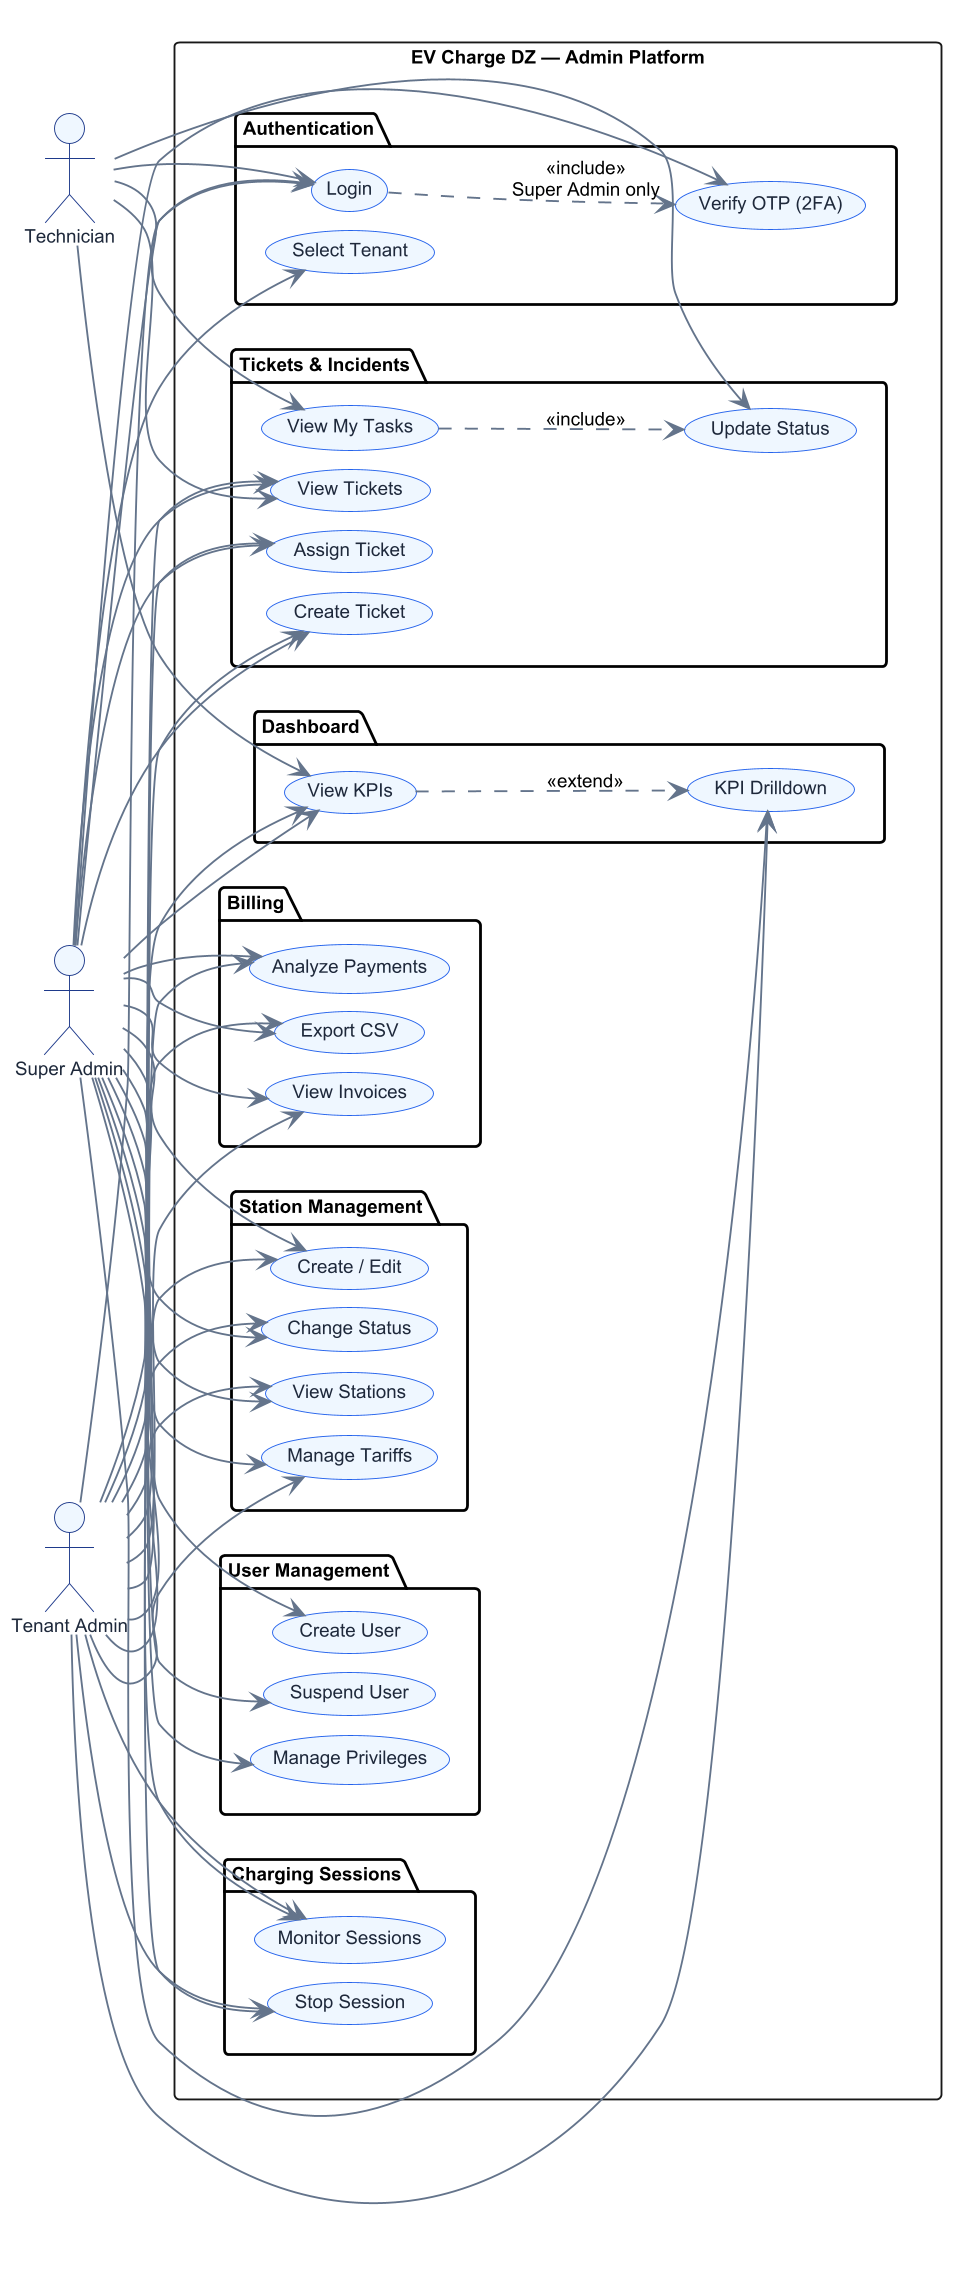
\includegraphics[width=0.72\textwidth, height=0.92\textheight, keepaspectratio]{../diagramme/UseCaseDiag.png}
  \caption{Combined Use Case Diagram --- All Actors}
  \label{fig:usecase-combined}
\end{figure}

\chapter{Complete Class Diagram (with Enumeration Types)}
\label{app:class-diagram-full}

The diagram below reproduces the full database-oriented class diagram of EV Charge DZ,
including all enumeration types (\texttt{UserRole}, \texttt{UserStatus},
\texttt{StationStatus}, \texttt{SessionStatus}, \texttt{TicketPriority},
\texttt{TicketStatus}, \texttt{TicketCategory}, \texttt{PaymentStatus},
\texttt{PaymentMethod}, \texttt{AlertSeverity}). These types are referenced as attribute
domains within the core entities but carry no inter-entity relationship; they are presented
here for completeness.

\begin{figure}[h]
  \centering
  \makebox[\textwidth]{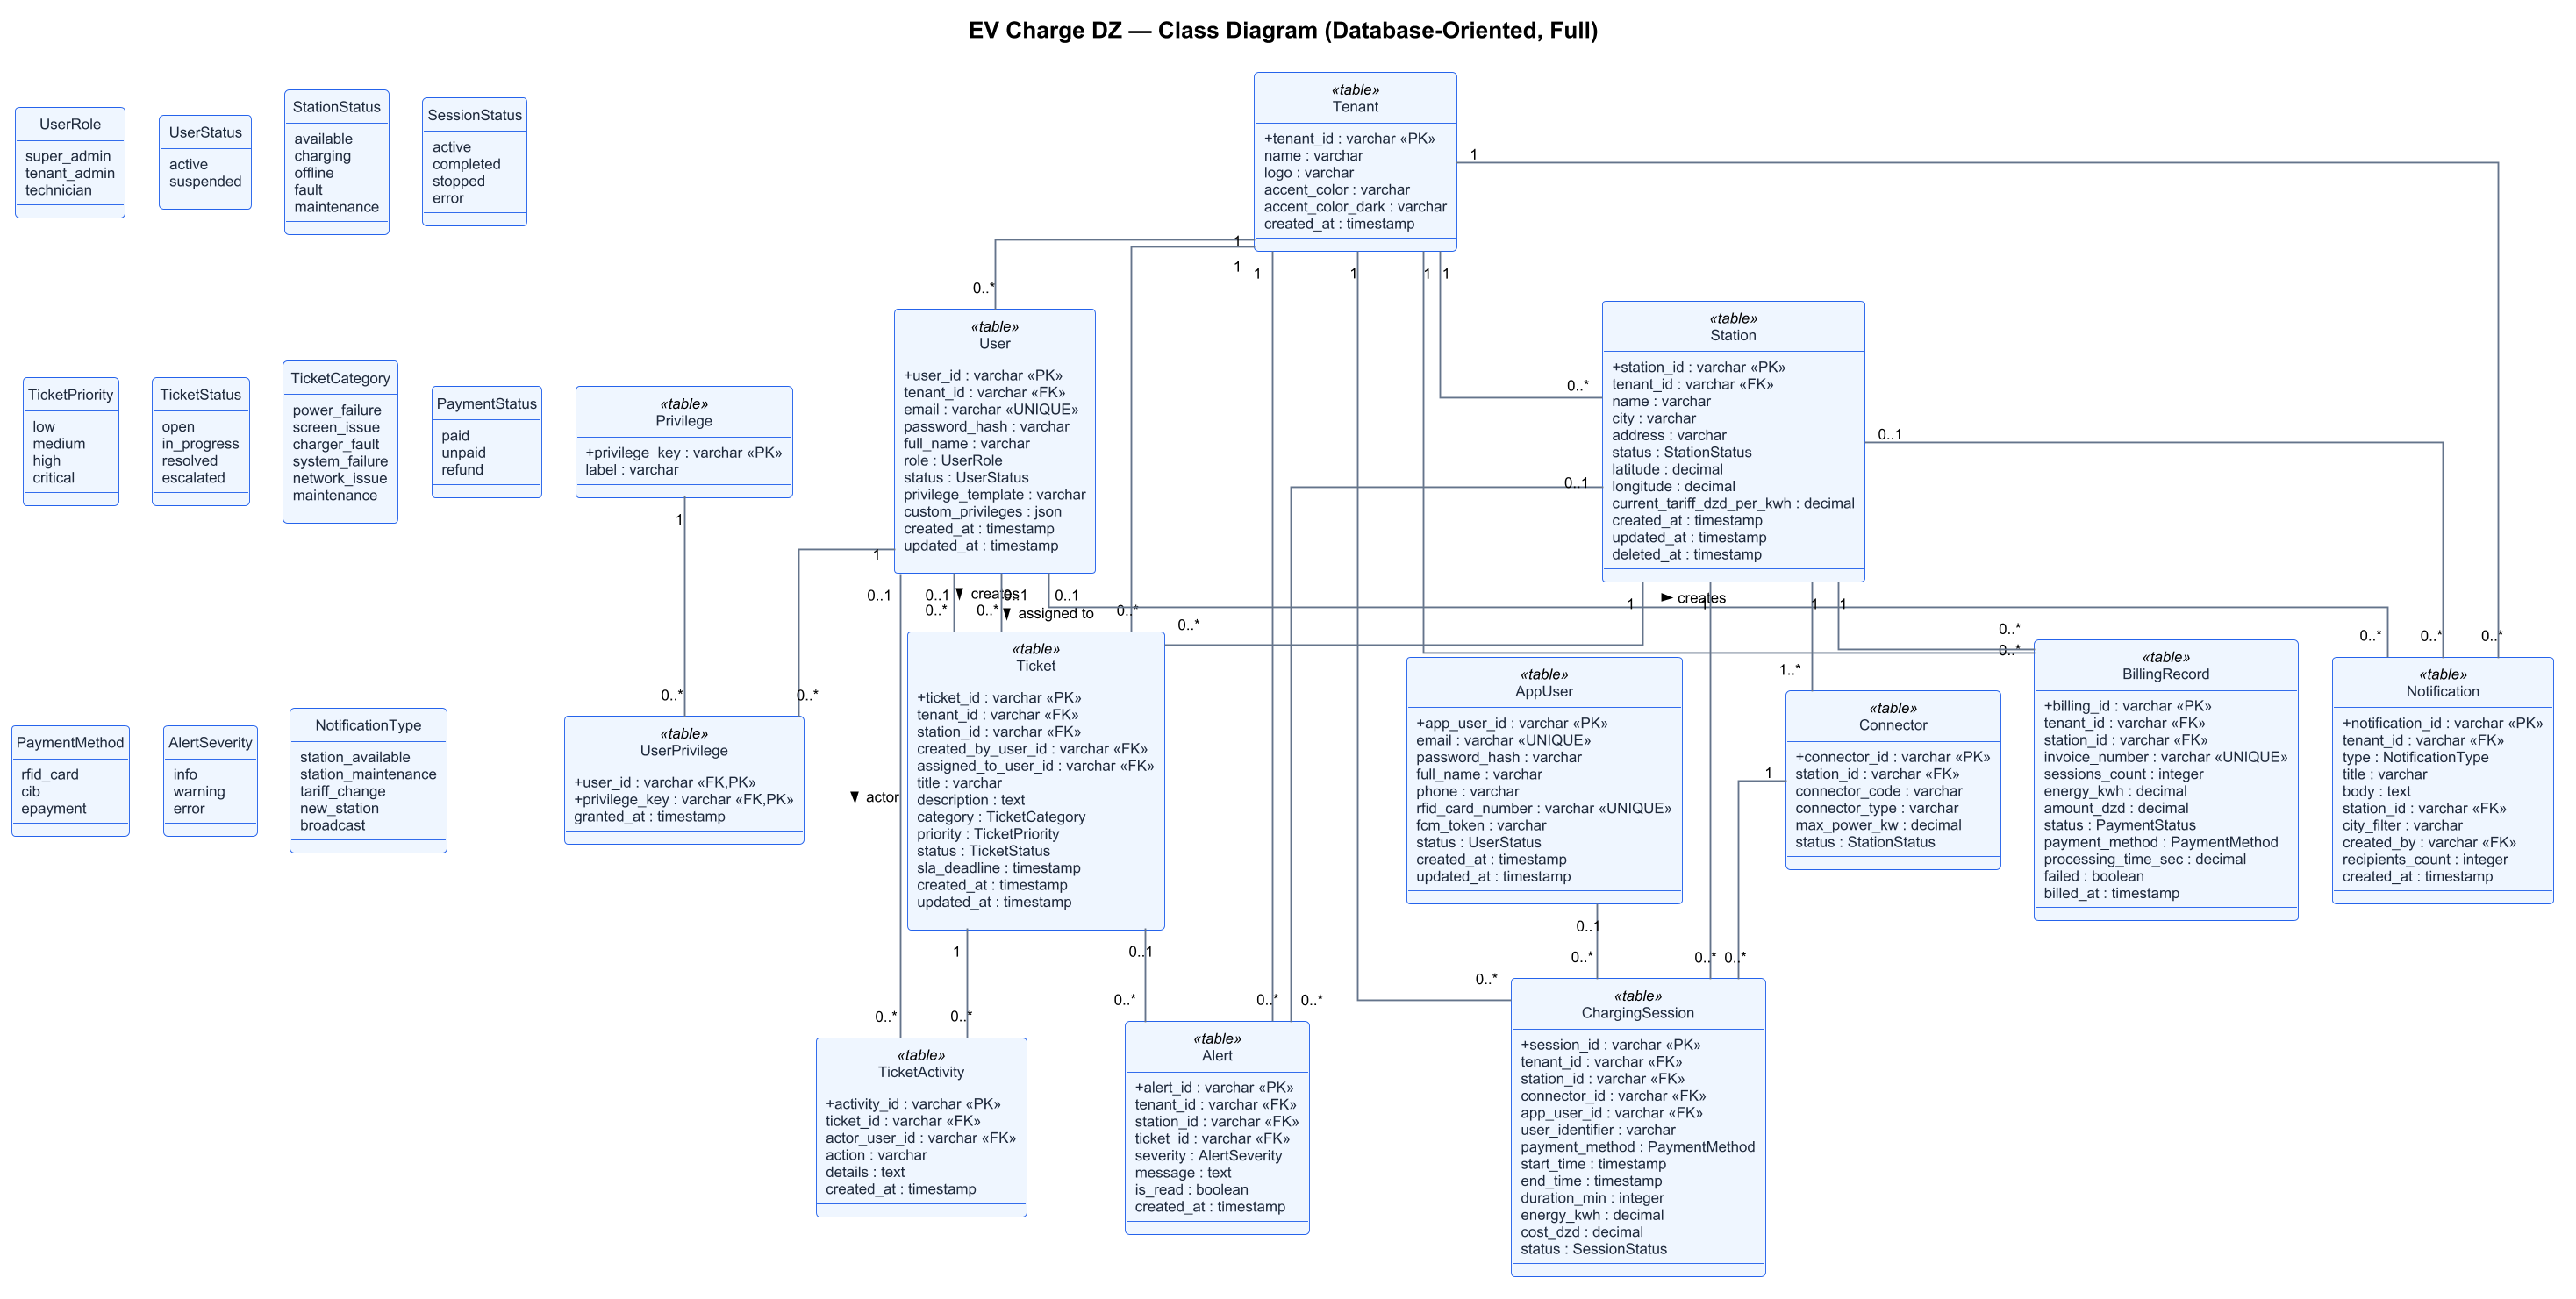
\includegraphics[width=1.25\textwidth, keepaspectratio]{../diagramme/DiagClass.png}}
  \caption{Full class diagram including enumeration types}
  \label{fig:class-diagram-full}
\end{figure}

\end{document}
